% --------------------------------------------------------------
% This is all preamble stuff that you don't have to worry about.
% Head down to where it says "Start here"
% --------------------------------------------------------------
 
\documentclass[12pt]{article}

\usepackage{enumitem, graphicx, amsmath, subcaption, wrapfig, setspace}
\usepackage{hyperref}
\usepackage{tabularx}
\usepackage{listings}
\usepackage{float}
\usepackage{caption}
\usepackage{csquotes}
\usepackage{color}
\usepackage[margin=1.11in]{geometry}
\setlist[description]{leftmargin=\parindent,labelindent=\parindent}
\graphicspath{ {./images/} }
\numberwithin{equation}{subsection}
 
\definecolor{codegreen}{rgb}{0,0.6,0}
\definecolor{codegray}{rgb}{0.5,0.5,0.5}
\definecolor{codepurple}{rgb}{0.58,0,0.82}
\definecolor{backcolour}{rgb}{0.95,0.95,0.92}
 
\lstdefinestyle{mystyle}{
    backgroundcolor=\color{backcolour},   
    commentstyle=\color{codegreen},
    keywordstyle=\color{magenta},
    numberstyle=\tiny\color{codegray},
    stringstyle=\color{codepurple},
    basicstyle=\footnotesize,
    breakatwhitespace=false,         
    breaklines=true,                 
    captionpos=b,                    
    keepspaces=true,                 
    numbers=left,                    
    numbersep=5pt,                  
    showspaces=false,                
    showstringspaces=false,
    showtabs=false,                  
    tabsize=2
}
 
\lstset{style=mystyle}

\renewcommand\lstlistingname{SrC Snippets}
\renewcommand\lstlistlistingname{Source Code Snippets}


%%%%%% Making LaTeX differentiation / integration much easier %%%%%%%
%%%%% See http://www.latex-community.org/forum/viewtopic.php?f=46&t=10000#p38694 %%%%%
%%%% or C. Beccari. TUGBoat 18 (1997) No. 1. %%%%
\makeatletter
\providecommand*{\diff}%
        {\@ifnextchar^{\DIfF}{\DIfF^{}}}
\def\DIfF^#1{%
        \mathop{\mathrm{\mathstrut d}}%
                \nolimits^{#1}\gobblespace
}
\def\gobblespace{%
        \futurelet\diffarg\opspace}
\def\opspace{%
        \let\DiffSpace\!%
        \ifx\diffarg(%
                \let\DiffSpace\relax
        \else
                \ifx\diffarg\[%
                        \let\DiffSpace\relax
                \else
                        \ifx\diffarg\{%
                                \let\DiffSpace\relax
                        \fi\fi\fi\DiffSpace}   
%%%%%% end here %%%%%%%

%%%% force indent command of paragraph in section %%%%
\newcommand{\forceindent}{\leavevmode{\parindent=1em\indent}}
%%%% end here %%%%

\begin{document}
% --------------------------------------------------------------
%                         Start here
% --------------------------------------------------------------
 
%%%%%
\onehalfspacing %Spacing
%\spacing{1.3}
%\linespacing{1.25}
%%%%%

\title{Understanding Baseball in an Analytical Fashion \\
Using Similarity Scores to Compare Team Performances and Player Performance}%replace X with the appropriate number
\author{Kai Chang\\ \\%replace with your name
Ay119, SP 2016} %if necessary, replace with your course title
 
\maketitle

\pagebreak

%%%%%%
\begin{abstract}
\noindent I've always been into baseball -- more for the stats than for the game itself. Don't get me wrong, the game is great, but what I love the game is what's behind it. Each action made can be contributed deep down to numbers, the statistics. For this AY class, I decided to focus on a number of my favorite aspects of baseball and some of the tasks I've always wanted to do, and attempt to complete them to an acceptable degree. This is rather a starting point into full analysis, and this will act as finding some preliminary results, whether it be successful or not. We focus on determining similarity scores within baseball teams across many seasons, visualizing the aspects or characteristics that either successful teams or non-successful teams share. This is particularly the grunt work, as we cover SQL/CSV queries, to implementing our own sabremetrics through effective programming practices, to isolating resulting data and interpreting through visual models. From here, we can expand further to apply our learning to individual major league players, and by finding similar players throughout history, we can then attempt to project performance of baseball players ten years down the road. We will compare the results to the PECOTA results.
\end{abstract}

\pagebreak

\tableofcontents
\lstlistoflistings

\pagebreak

%%%%%%%
\section{Introduction}
"Baseball is a sport dominated by statistics."\cite{Bales} Every part of the game is statistic based, and most scenarios are binary based. Although players, like variables in nature, and bound by Gaussian tendencies, baseball seems unpredictable. However, many sabremetrics will argue that the reason can be explained behind the number, and there is a lot of it. Baseball stats have been recorded since the late 19th century, where the sport first began, and the current day database contains numbers describing the exact pitch in a game. This large database and statistical tendencies in the sport make baseball the perfect dataset.

Baseball is a data-driven sport, more so than others. "What we’re looking for in any stat is that it can help us make better predictions. When it comes down to it, that’s all we need; if a stat can’t lead to actionable insights, it’s really of no use to us."\cite{Bales}

\subsection{Objectives}
Thus, the goal of this project is to understand the current state of baseball, and potentially project stats in the future. The most important aspect is focusing on similarities between entities, either players or teams. So, we look into analyzing and quantifying similar team performances across time, beyond wins and losses. From gaining this insight, we can then apply this to quantifying similarity scores in players, and by gathering similar players, we can use their later years to project the statistics of our desired player years (up to 10) down the road. This can be compared to the current PECOTA numbers, and down the road, when the events play out, we can determine which one is more accurate.

It's important to start at the team level, because of the sample size of the team data relative to the individual player data. Once the analysis is successful on the team data, only then can we apply it to a much larger mapping of player data (with season frames).

\textit{What is meant by season frames is this: a team season performance are individual and only respective to that season -- one cannot combine multiple seasons of the same team due to the constant change in rosters, so queries of similar performances are limited to 1 season or 1 datapoint (vector). An individual player, however, can query multiple seasons to better gauge similarities, meaning the search is much more difficult.}


\section{Understanding Statistics}
It's important to understand the statistics we use and develop to determine a similarity score between two players. These statistics fall into three categories: traditional statistics, or statistics that have been used universally for some time now, professional sabremetrics, or statistics that have been developed to give a more weighted understanding of performance, and individualized sabremetrics, or statistics personally developed that I felt current sabremetrics lacked.

\subsection{Traditional Statistics}
\subsubsection{OPB}
OBP or \textbf{On Base Percentage} is a statistic used to measure how often a batter gets on base. The formula is given by
\begin{equation}
	OBP = \frac{H + BB + HBP}{AB + BB + HBP + SF}
\end{equation}
where $H$ is hits by batter, $BB$ is walks by batter, $HBP$ is times batter is hit by pitch, $AB$ is total at bats, and $SF$ is sacrifice flies made by batter. This is an independent statistic from average because it takes into accounts sacrifices made by batters to improve chances of team success. Higher OPB suggests more successful hitters.

\subsubsection{SLG}
SLG or \textbf{Slugging Percentage} is a statistic used to measure how much power a batter has. The formula, given by
\begin{equation}
	SLG = \frac{1B + 2\times 2B + 3\times 3B + 4\times HR}{AB}
\end{equation}
where $1B$ is singles, $2B$ is doubles, $3B$ is triples, and $HR$ represents home runs made. SLG is an elementary way of differentiating production amongst hitters, giving weight to those hits that provide a higher probability of scoring. Higher SLG suggests more successful hitters.

\subsubsection{ERA}
ERA or \textbf{Earned Run Average} is a statistic used to measure the earned runs a player would give up in a traditional nine-inning game. The formula is given by
\begin{equation}
	ERA = 9 \times \frac{ER}{IP}
\end{equation}
where $ER$ stands for the number of earned runs (runs minus errors made by fielding), and $IP$ represents the innings pitched. Henry Chadwick first invented this statistic to measure the effectiveness of pitchers. Lower ERA suggests more successful pitchers.

\subsubsection{WHIP}
WHIP or \textbf{Walks Plus Hits per Inning Pitched} is a measurement of the number of base runners a pitcher allows in an inning. The formula, given by
\begin{equation}
	WHIP = \frac{BB + H}{IP}
\end{equation}
helps give an additional aspect to a player besides giving up runs. It provides an understanding of the tendency for a player to allow batters to reach base. Lower WHIP suggests more successful pitchers.

\subsection{Professional Sabremetrics}
\subsubsection{BABIP}
BABIP or \textbf{Batting Average on Balls in Play} measures the tendency for a ball in play play to be recorded as a hit. 

\begin{equation}
	BABIP = \frac{H-HR}{AB-SO-HR+SF}
\end{equation}
where $SO$ represents the strikeouts of the player.
BABIP is a step above average because it has a tendency to account for luck. We can notice that a player whose BABIP is much higher or lower that his average BABIP can be accounted for by good or bad luck. "If a player has a BABIP of .450 over his last 10 games, it’s a sign that he’s gotten really lucky; perhaps it was the location of his hits or poor defense, but no one will maintain a .450 BABIP over the long run."\cite{Bales}. Note the average BABIP is around 0.300.

\subsubsection{wOBA}
wOBA or \textbf{Weighted On-Base Average} is a measurement that values certain hits more than others. wOBA values distributes the weights of hits according to their probabilities to score for a team. From fangraphs\cite{fangraphs}: 

\begin{displayquote}
Batting average assumes that they are. On-base percentage does too, but does one better by including other ways of reaching base such as walking or being hit by a pitch. Slugging percentage weights hits, but not accurately (Is a double worth twice as much as a single? In short, no) and again ignores other ways of reaching base. On-base plus slugging (OPS) does attempt to combine the different aspects of hitting into one metric, but it assumes that one percentage point of SLG is the same as that of OBP. In reality, a handy estimate is that OBP is around twice as valuable than SLG (the exact ratio is x1.8). In short, OPS is asking the right question, but we can arrive at a more accurate number quite easily.

Weighted On-Base Average combines all the different aspects of hitting into one metric, weighting each of them in proportion to their actual run value. While batting average, on-base percentage, and slugging percentage fall short in accuracy and scope, wOBA measures and captures offensive value more accurately and comprehensively. 

\end{displayquote}

\begin{equation}
	wOBA = \frac{0.75\times BB + 0.9\times HBP + 0.89\times 1B + 1.24 \times 2B + 1.56 \times 3B + 1.95 \times HR}{PA}
\end{equation}
where $PA$ represents a batter's total plate appearance (different from at bats).

Note that wOBA varies across all sites, but for this case study, we approximate wOBA as such, based on our truncated data.

\subsubsection{FIP}
FIP or \textbf{Field Independent Pitching} measures a pitchers performance without defense. None of the statistics that are defensive dependent are involved.

\begin{equation}
	FIP = \frac{13\times HR + 3\times (BB + HBP) - 2 \times SO}{IP} + FIP\_Constant
\end{equation}
where in our case the $FIP\_Constant$ is zero. This looks past the ERA and gives more weight to those pitchers that can strike out more, which is typically more dominant pitchers. However, this may overlook pitchers that rely on fielding as a groundball pitcher.

\subsubsection{PBABIP}
PBABIP is given in the same context as a batter's BABIP, but now for how lucky or how effective some pitcher are. When a pitcher has a high BABIP, it suggests that an improvement of performance is in the future. However, with a low BABIP, the opposite can be applied. BABIP is lower for those that rely on fielders or groundball pitchers.

\begin{equation}
	PBABIP = \frac{HA - HRA}{(IPouts + HA + HRA + BBA + SOA)-BBA - HRA + DP/4.00 - E/8.00}
\end{equation}
where $HA$ is hits allowed, $HRA$ is home runs allowed, $IPouts$ is total outs pitched, $BBA$ is walks allowed, $SOA$ is strike outs allowed, $DP$ is double plays, and $E$ is errors. Note this is slightly different from other PBABIP as this includes $DP$ and $E$.

\subsection{Individualized Sabremetrics}
\subsubsection{effERA}
The effERA or \textbf{Effective ERA} is a self-developed statistic that determines an earned run average score by awarding the pitcher for complete games and shutouts, while penalizing the pitcher for having relief pitchers pitch, and homers allowed. The effective ERA is a take on the ERA of a pitcher from the pressures and environments around him or her.

\begin{equation}
	effERA = ERA - 0.018\times SHO - 0.006 \times CG + 0.002 \times HRA + 0.0015 \times SV + (1.00 - FP)/2
\end{equation}
where $SHO$ is shutouts pitched, $CG$ is complete games pitched, $SV$ represents saves and $FP$ is fielding percentage.

Note that this is for team statistics, because this effERA would not work for closers (with high SVs) or pitchers (who don't usually incur saves). To modify this effERA for individual players, SV coefficients would need to be adjusted. Fielding Percentage would also need to be reweighed to include accurate statistic.

\subsubsection{Complete Game Rate}
The complete game rate is a statistic looking into how dominant a team's starting rotation is. It is suggestive that better pitchers throw more complete games, either through their endurance, or through the box score. This can be both a pitcher and team statistic.

\begin{equation}
	CGRate = \frac{CG}{IPouts/27}
\end{equation}

\section{Procedure}
In order to tackle this project, we went through the following steps.
\begin{itemize}
	\item First, we took the SQL and CVS files from the Lahman's Baseball Database, updated up to 2015. Within this database contains lots of tables for every possible datapoint.
    \begin{figure}[H]
	\centering
	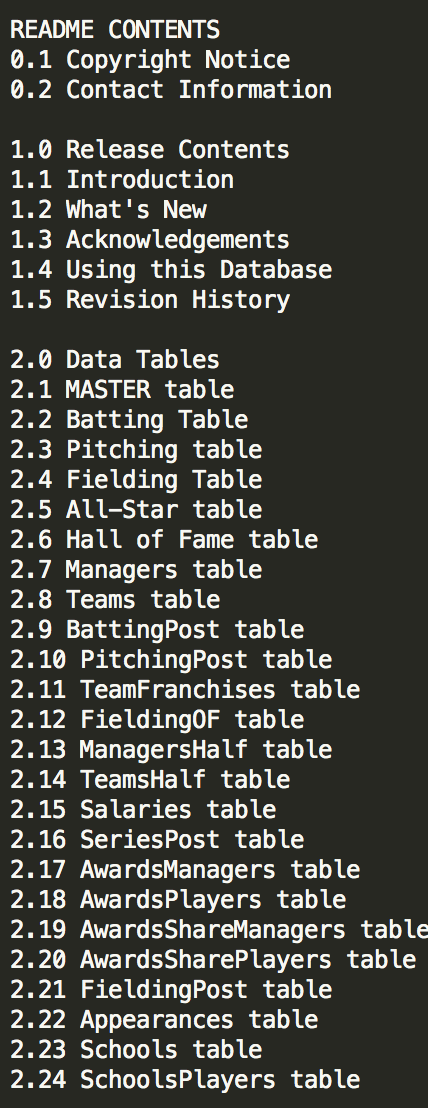
\includegraphics[width=0.25\textwidth]{tables}
	\end{figure}
    \item Familiarize self with R and SQL. In order to compare players at a fast rate, we will need to understand how queries run within R. 
    \item Develop similarity algorithm or method for teams, taking in CVS datafiles.
    \item Apply algorithm to a number of current teams, running the program to compare select team to historical teams. Then, we store the similarity scores for both batting and pitching.
    \item Visualize data with sabremetric statistics results from our refined query/computation CVS file.
    \item Interpreting any potential groupings or traits, apply PCA methods. We then see if the groupings developed share similar similarity scores as the ones computed. If so, then our algorithm and sabremetric tools were successful, and the same can be modified and applied to individual players.
\end{itemize}

\section{Database / Algorithm}
\subsection{R}
We first needed to experiment with databases through R and SQL/CVS. This is reasonable as the player database has a lot more components, and will need a more powerful program.
Thus, we followed and manipulated with the module \href{http://cpsievert.github.io/baseballR/20140818/}{\textit{Interactive animations of PITCHf/x with animint and pitchRx}} and \href{http://cpsievert.github.io/pitchRx/}{\textit{Introduction to pitchRx package}}. From these \href{https://www.datascienceriot.com/how-to-create-a-pitchfx-database-with-pitchrx-and-r/kris/}{modules}, we learned how to pull the PITCHf/x data straight from MLB, which is a database of all pitches thrown up to the detail of spin rate, velocity, and movement. We also learned how to collect data from an online database, manage data in R, and visualize it in 2D and 3D. Although this did not directly apply to the analysis, it did give me more insight into my analysis. 
\begin{figure}[H]
	\centering
	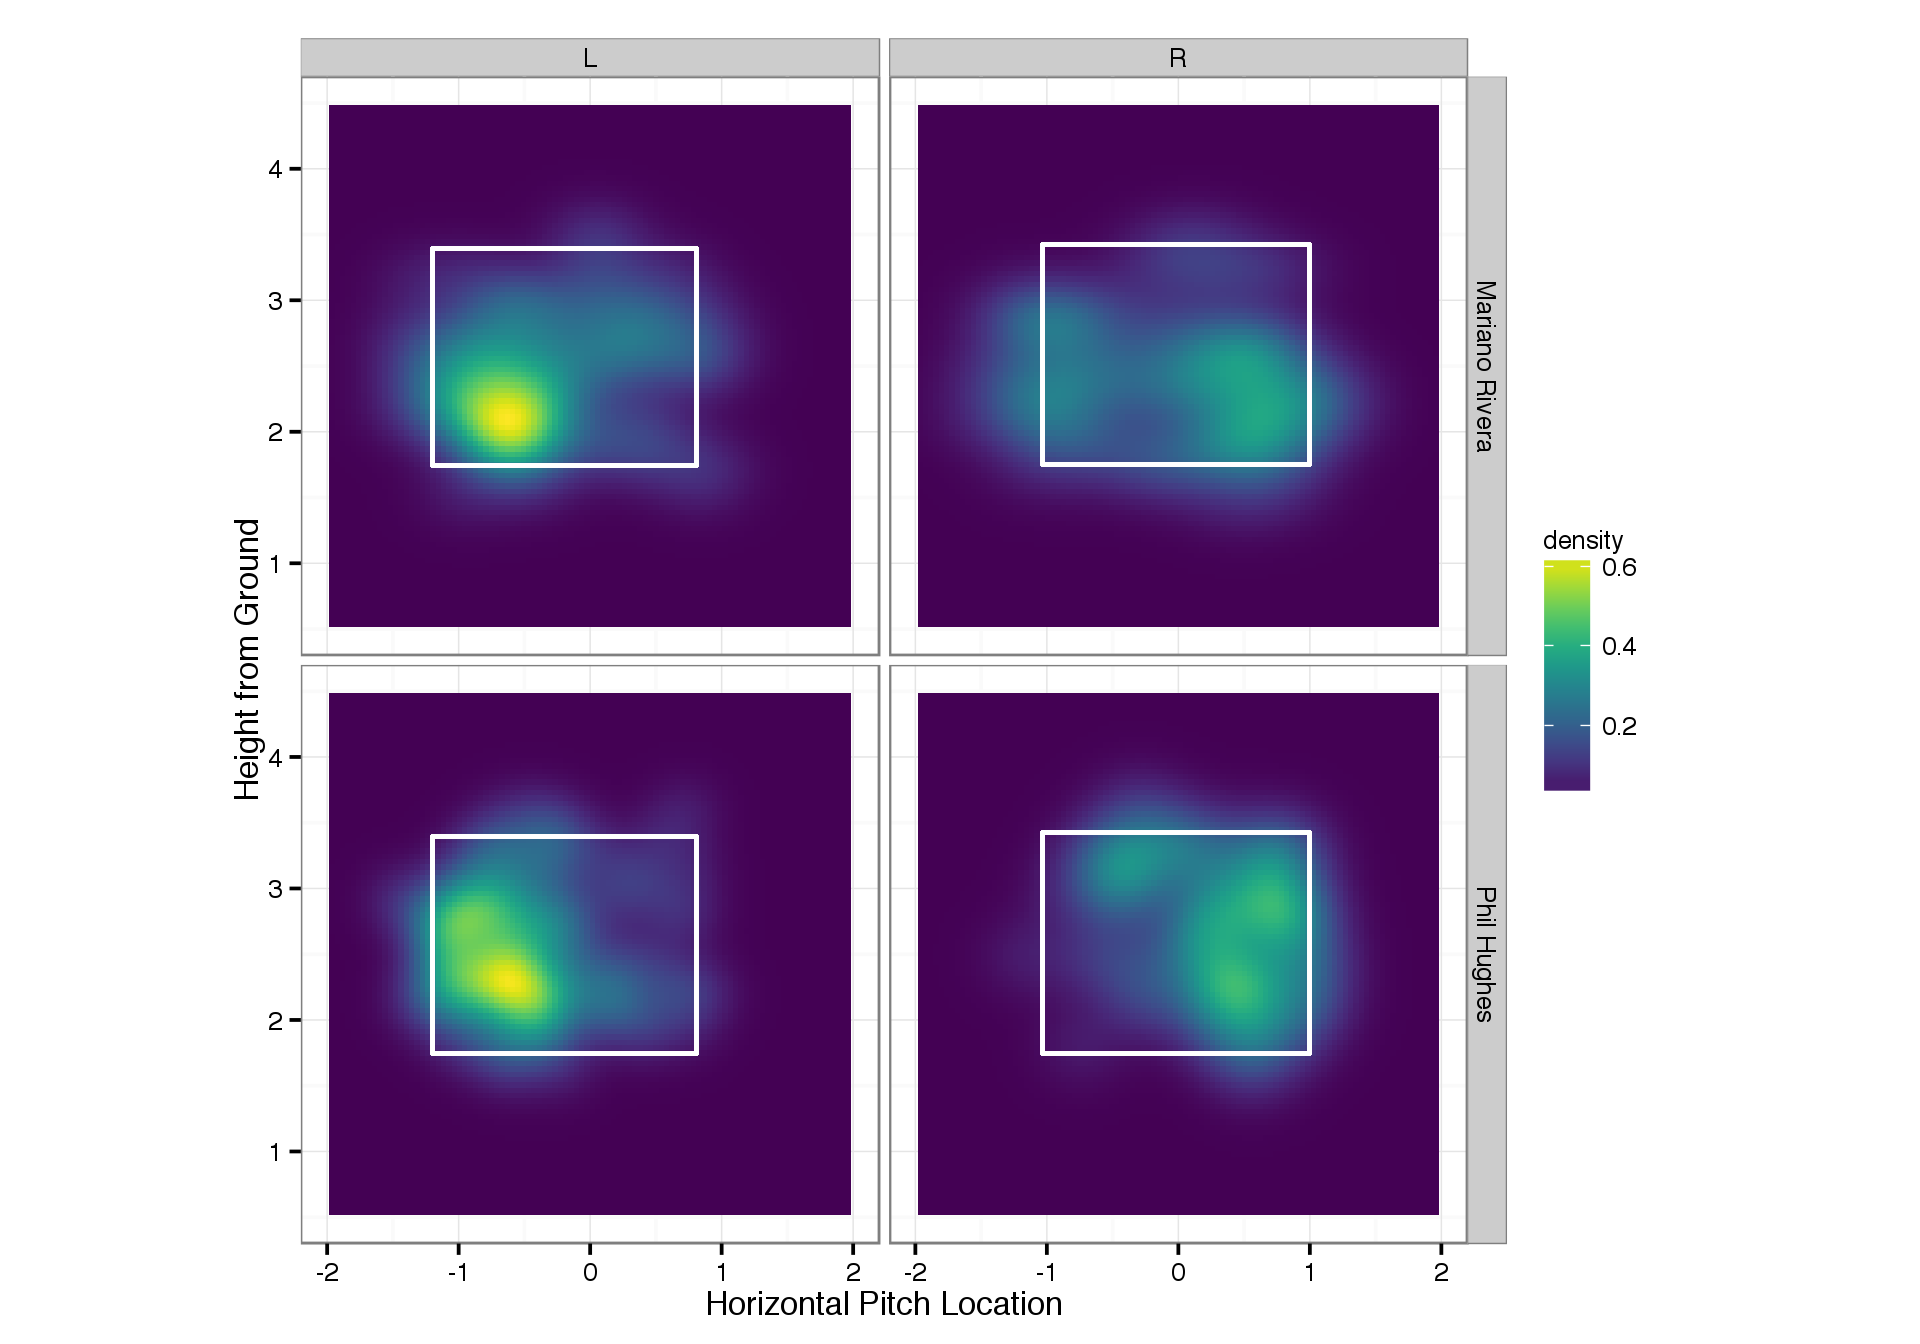
\includegraphics[width=0.5\textwidth]{index}
\end{figure}
This is very cool stuff, which I may consider later -- heat maps, pitch frames, groupings. This can be used down the line to help with similarity calculations. 

\begin{figure}[H] 
  \begin{subfigure}[b]{0.5\linewidth}
    \centering
    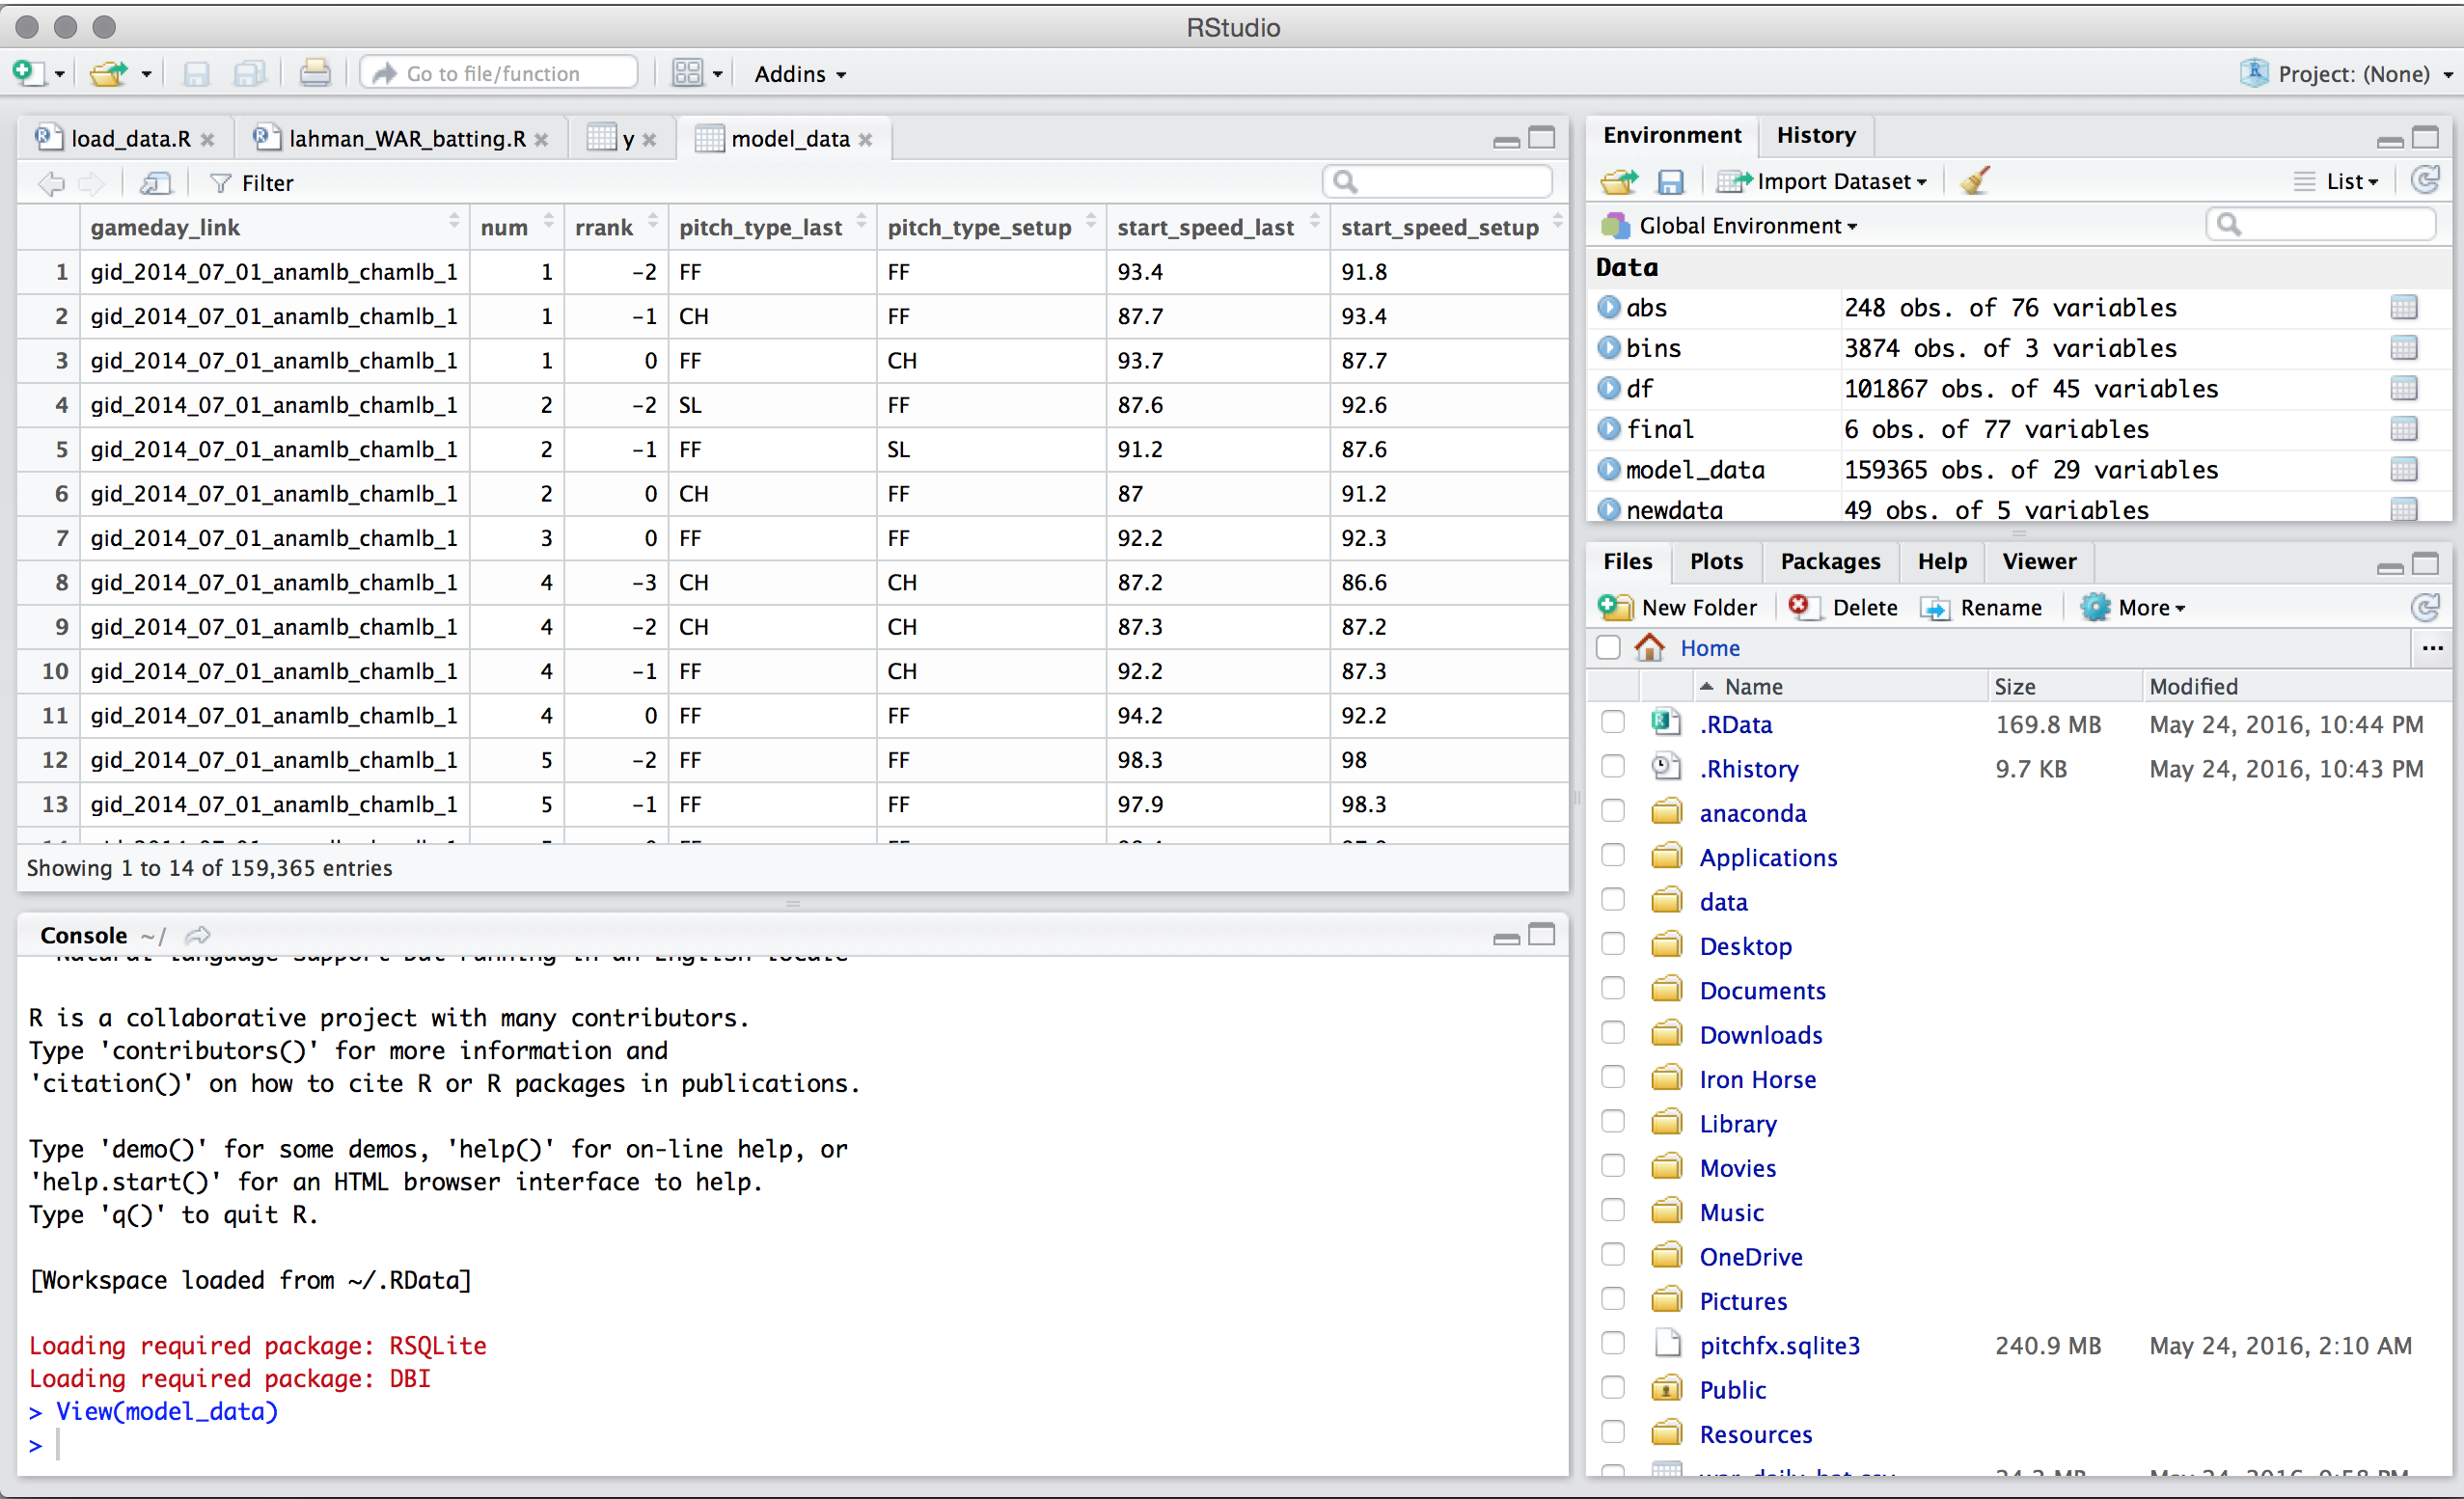
\includegraphics[width=0.7\linewidth]{rstudio} 
    \captionsetup{justification=centering}
    \label{fig2:a} 
    \vspace{4ex}
  \end{subfigure}%% 
  \begin{subfigure}[b]{0.5\linewidth}
    \centering
    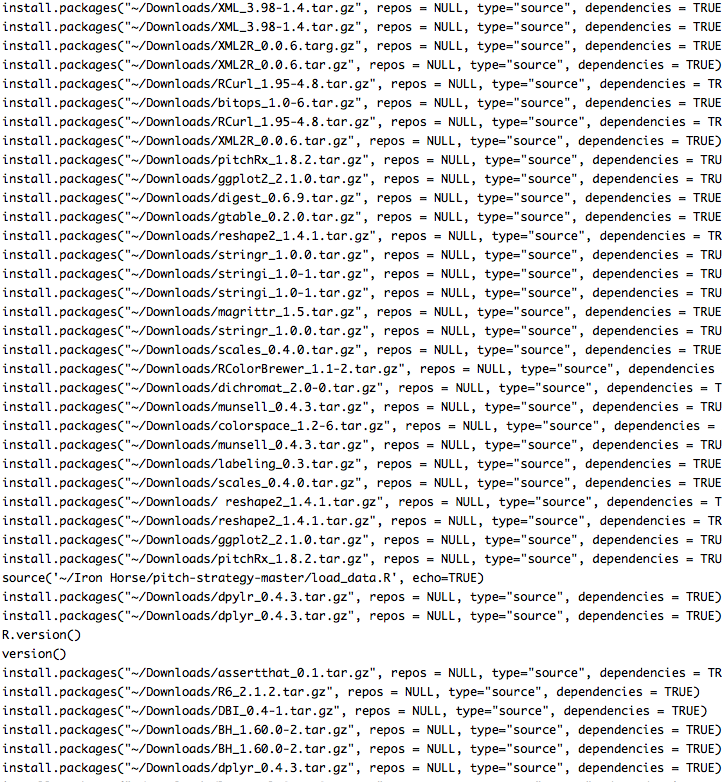
\includegraphics[width=0.7\linewidth]{rpackages} 
    \captionsetup{justification=centering}
    \label{fig2:b} 
    \vspace{4ex}
  \end{subfigure} 
  \caption{2014 Results in various binnings}
\end{figure}

I also played around with RStudio a bit, getting help with a Github tutorial to extract data, learning R along the way. R is now set up for any baseball analytics task.

\subsection{Python} %%%%%%%%%%
The full grunt of the work was written in Python. We imported our CSV files, and the program normalized each team's sabremetric as vectors to that season's league average. Then it calculated the similarities between the two by deriving at a score using the sabremetric statistics. From there, we saved the resulting data to a CSV to be visualized and further analyzed down the road. We compared each individual team from seasons 2012-2015 to each individual team's performance from season 1960-2015. 

\begin{figure}[H]
	\centering
	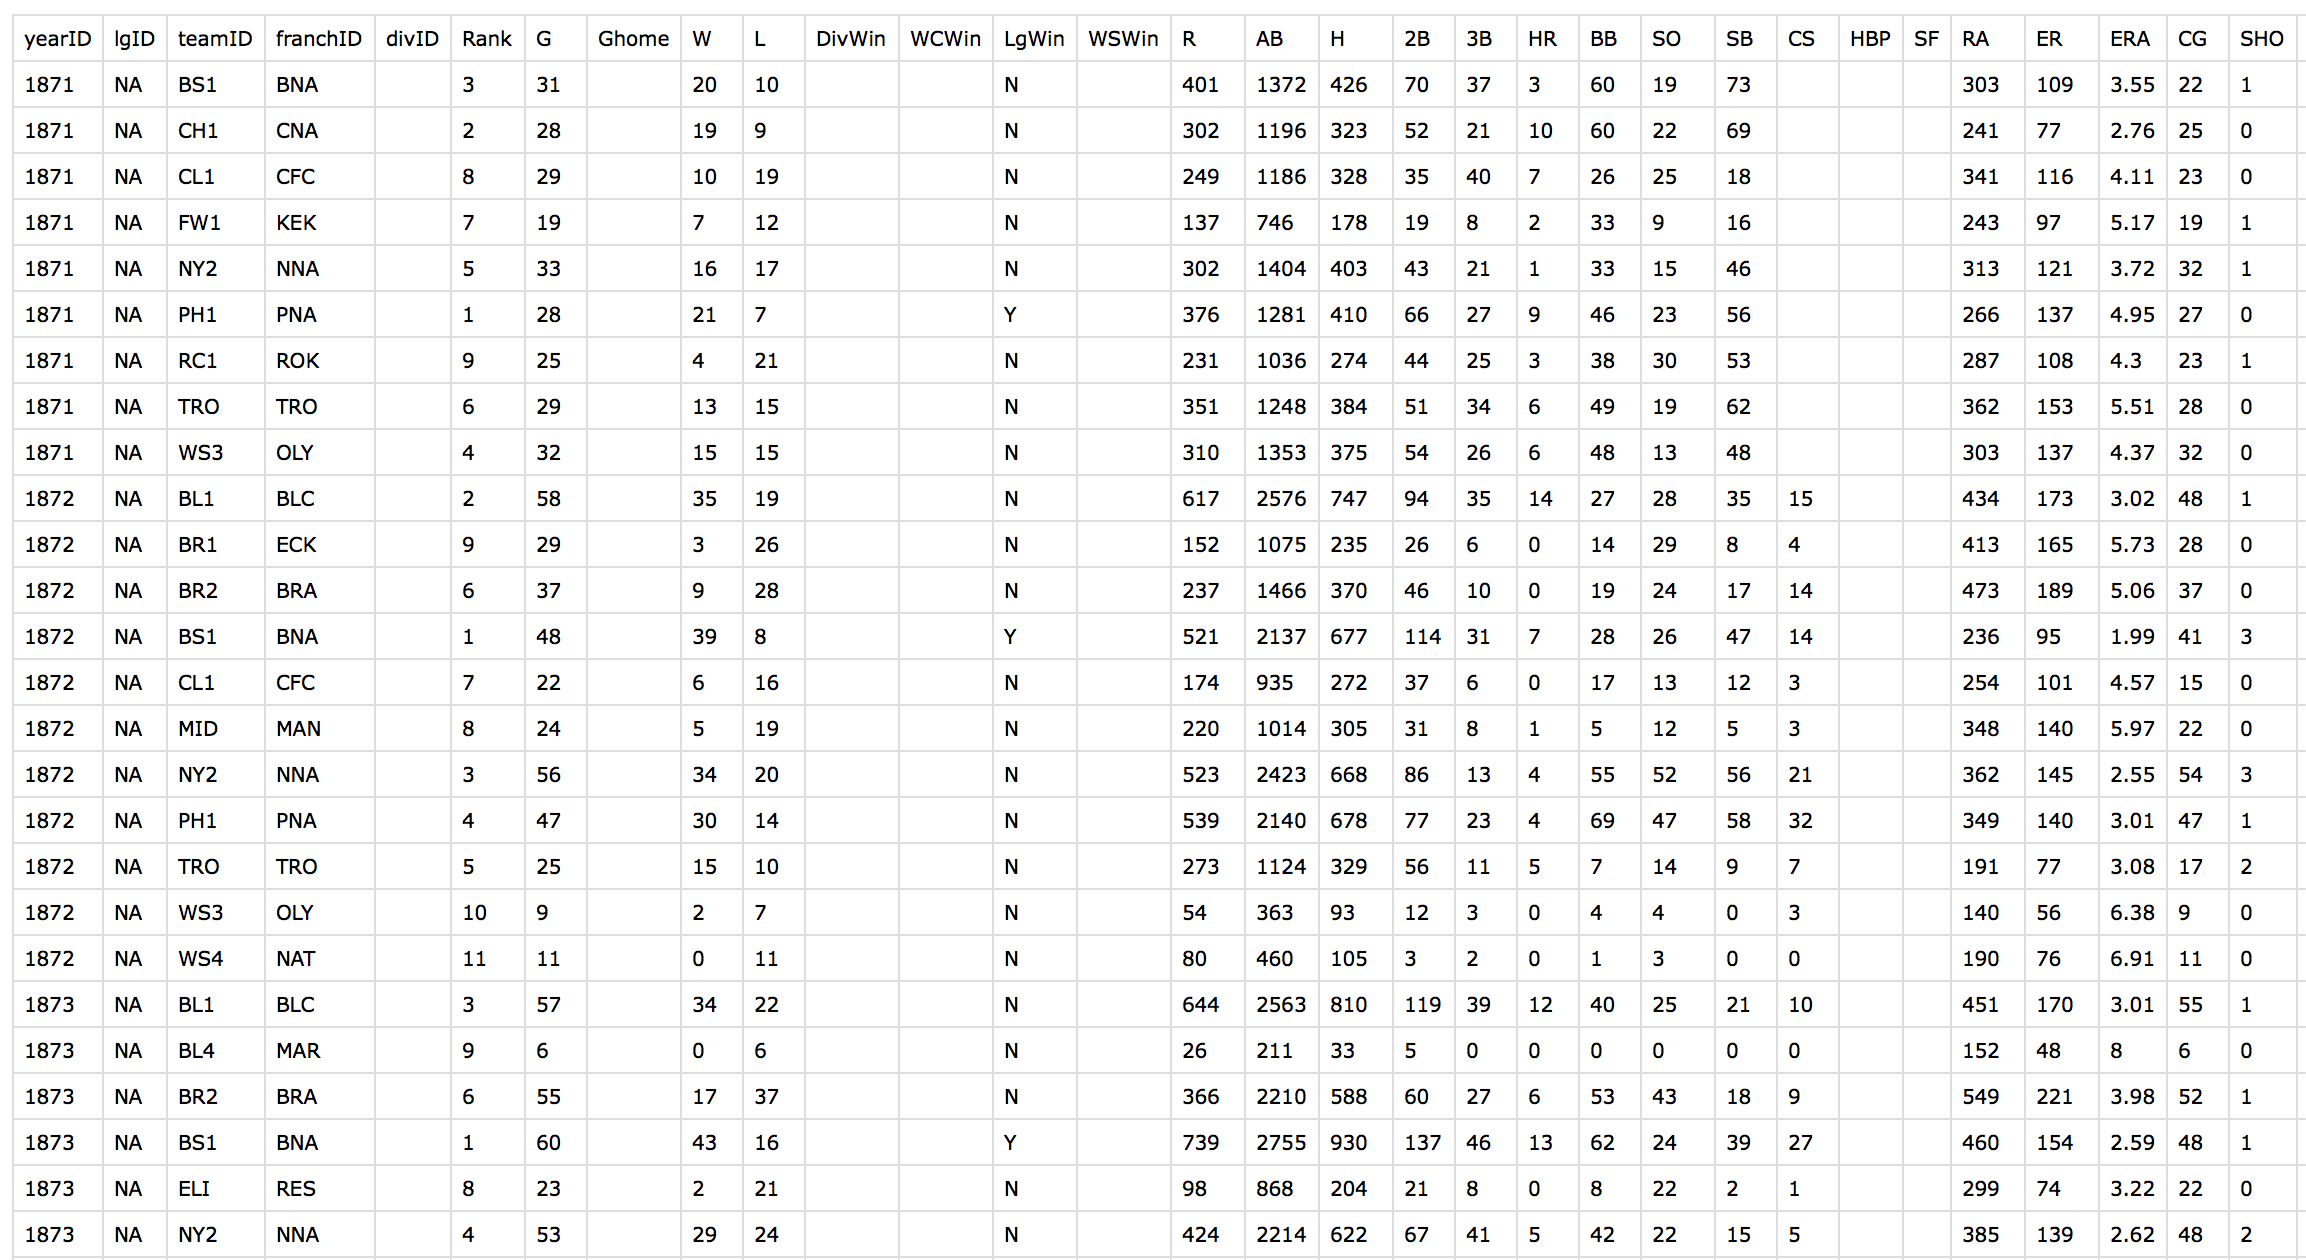
\includegraphics[width=0.9\textwidth]{python1}
    \caption{RAW CSV files from Lahman's Baseball Database}
\end{figure}

\begin{figure}[H]
	\centering
	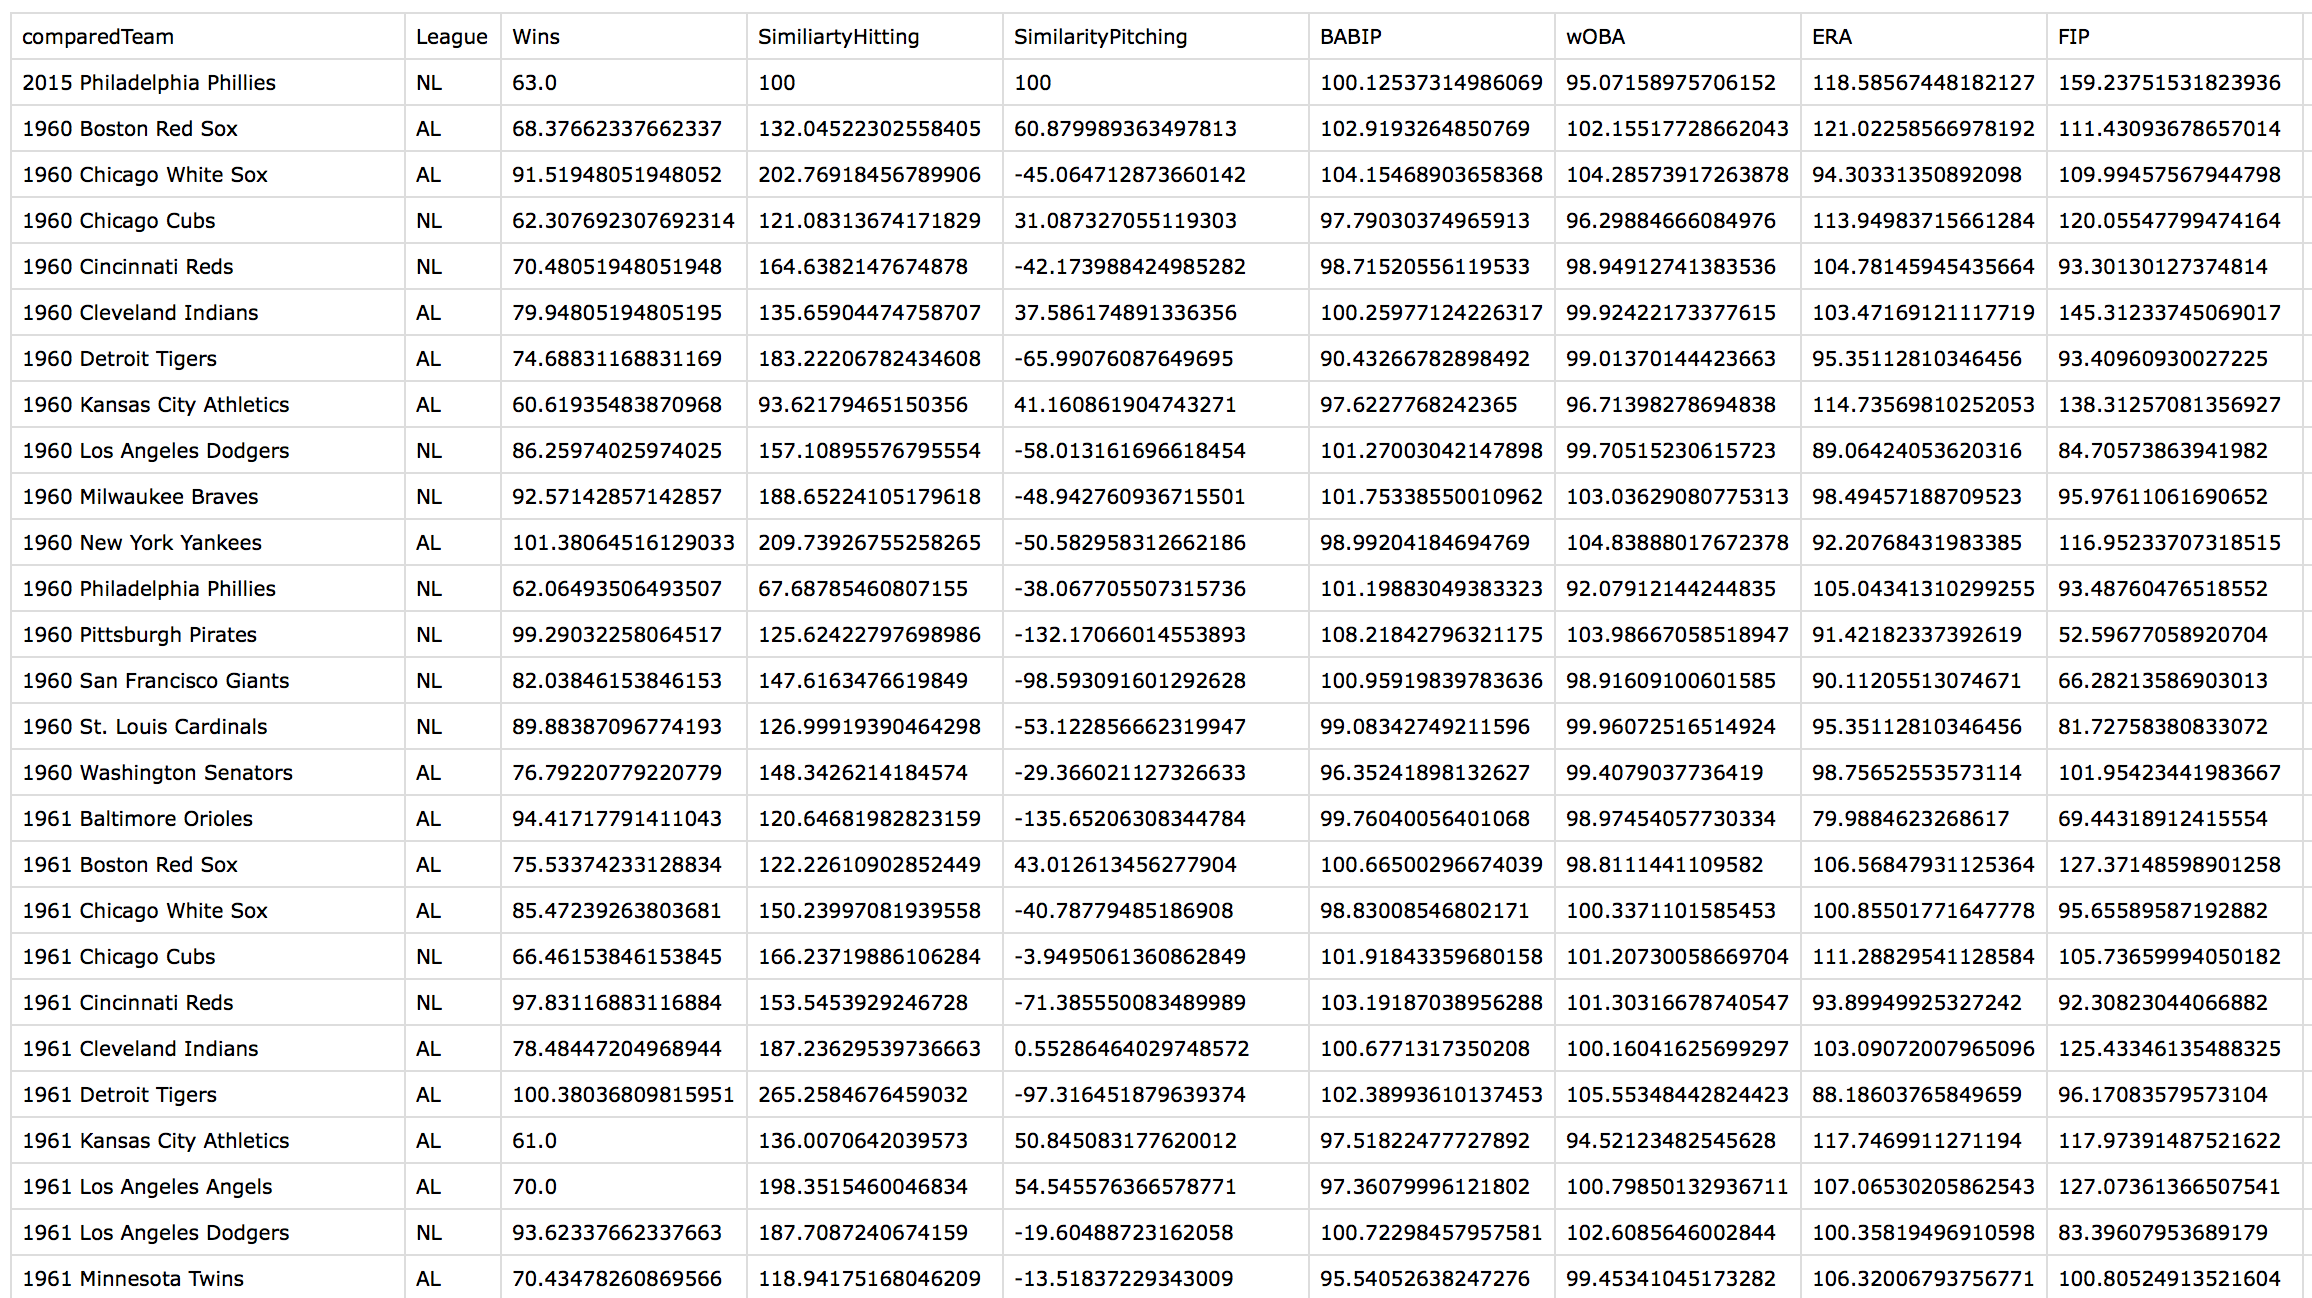
\includegraphics[width=0.9\textwidth]{python2}
    \caption{Similarity CSV created from program}
\end{figure}

Each of the values were normalized with respect to the season league average, and scaled appropriately such that 100 represented the league average. The similarity score is represented such that 100 defines identical performance (ie. the first team has a 100, 100 for batting, pitching because they are comparing to themselves). The interpretation for the normalize scores for the sabremetrics can be described as

\begin{itemize}
	\item Wins: Higher = better
	\item SimilarityHitting: $>100$ = better than target team
    \item SimilarityPitching: $<100$ = better than target team
    \item BABIP, WOBA: $>100$ = better than league average
    \item ERA, FIP, PBABIP, effERA: $<100$ = better than league average 
\end{itemize}

A preliminary examination of study showed that there are similarities between teams across time periods. A quick comparison between two teams from our first CSV file, 2012 Atlanta Braves, suggests that the 2012 Atlanta Braves and the 2014 Los Angeles Dodgers shared similar similarity scores (BS=107.38, PS=103.11). When we compare the two team's statistics online, we see at first glance that it doesn't seem very likely the two teams are similar. 

\begin{figure}[H]
	\centering
	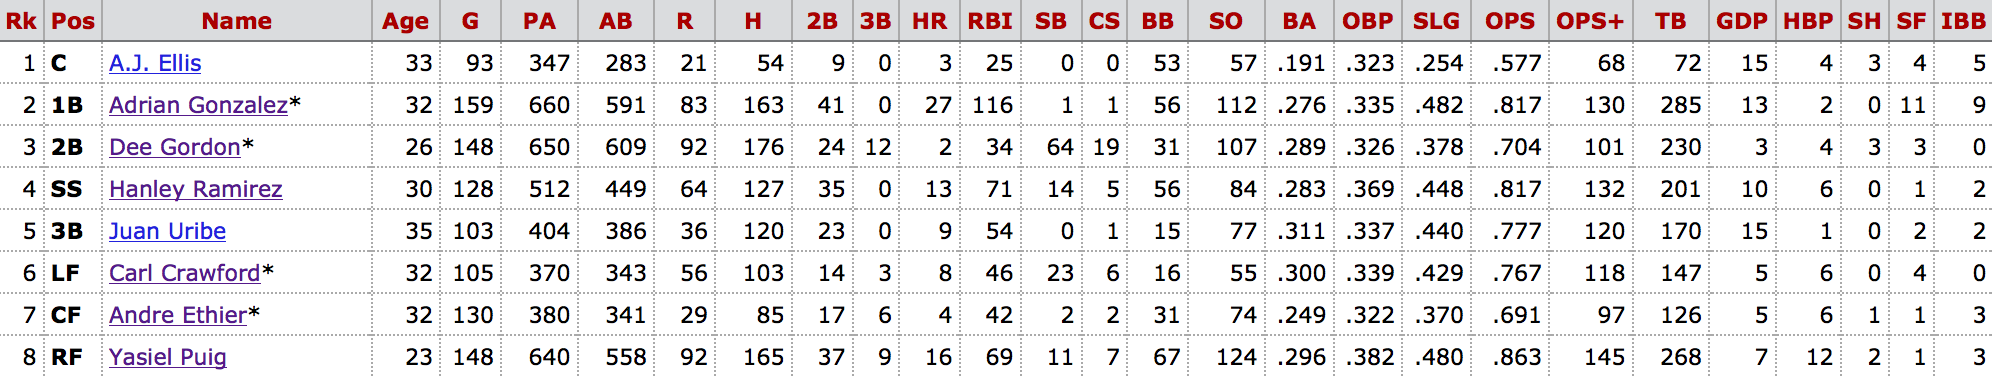
\includegraphics[width=0.9\textwidth]{dodgers1}
    \caption{Dodgers batting}
\end{figure}

\begin{figure}[H]
	\centering
	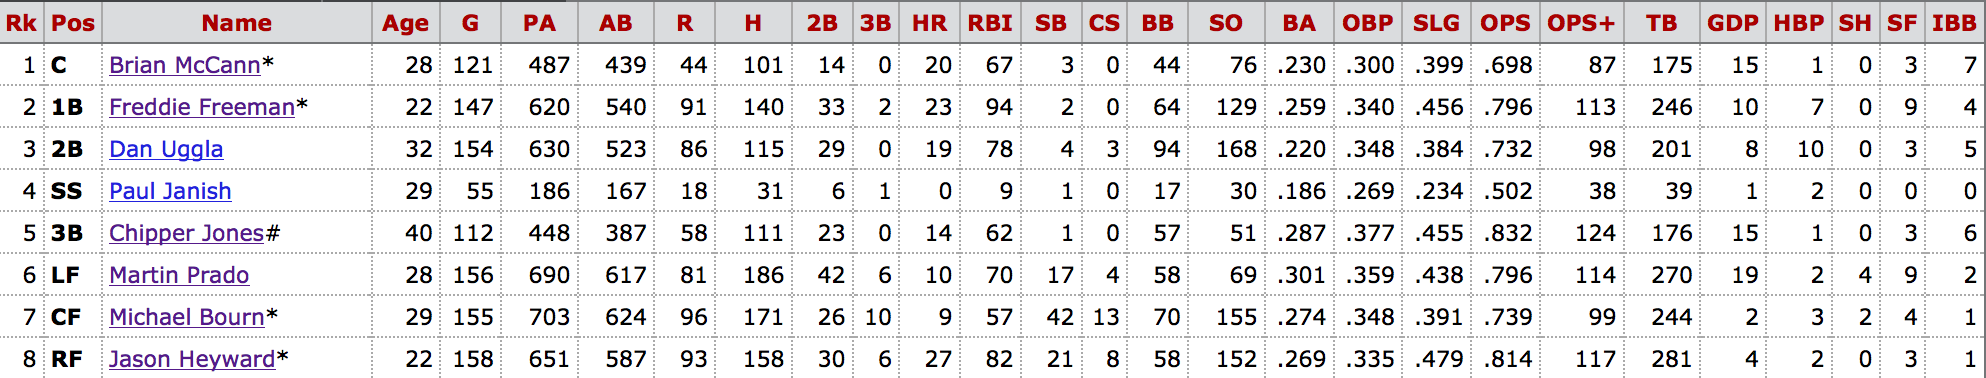
\includegraphics[width=0.9\textwidth]{braves1}
    \caption{Braves batting}
\end{figure}

\begin{figure}[H]
	\centering
	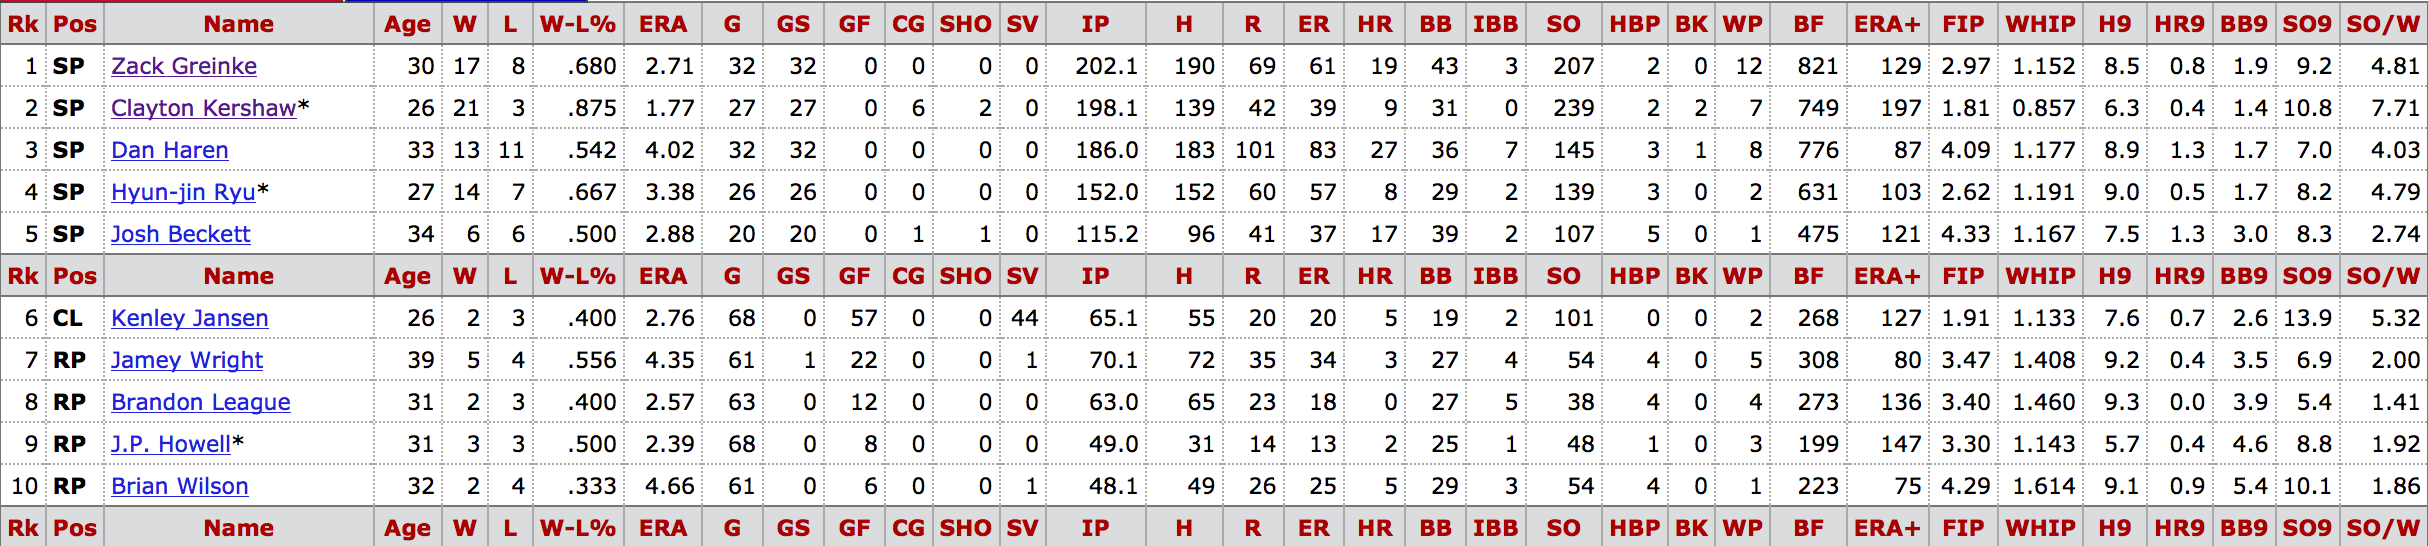
\includegraphics[width=0.9\textwidth]{dodgers2}
    \caption{Dodgers pitching}
\end{figure}

\begin{figure}[H]
	\centering
	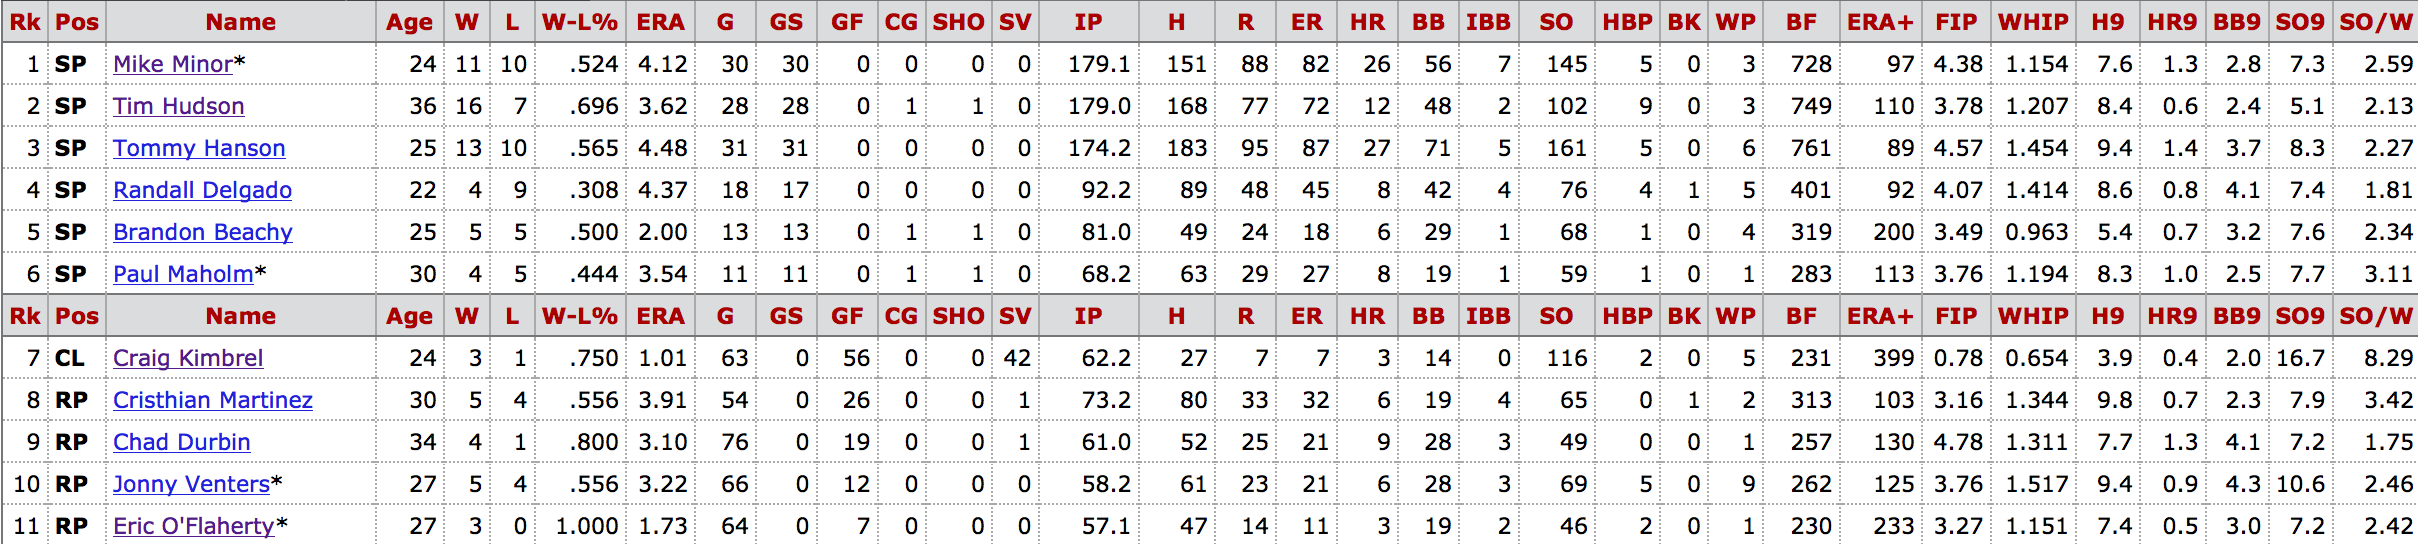
\includegraphics[width=0.9\textwidth]{braves2}
    \caption{Braves pitching}
\end{figure}

However, upon closer examination, looking beyond traditional statistics and into where the teams stood during the season, it becomes more apparent the similarity between the two teams.

\begin{figure}[H]
	\centering
	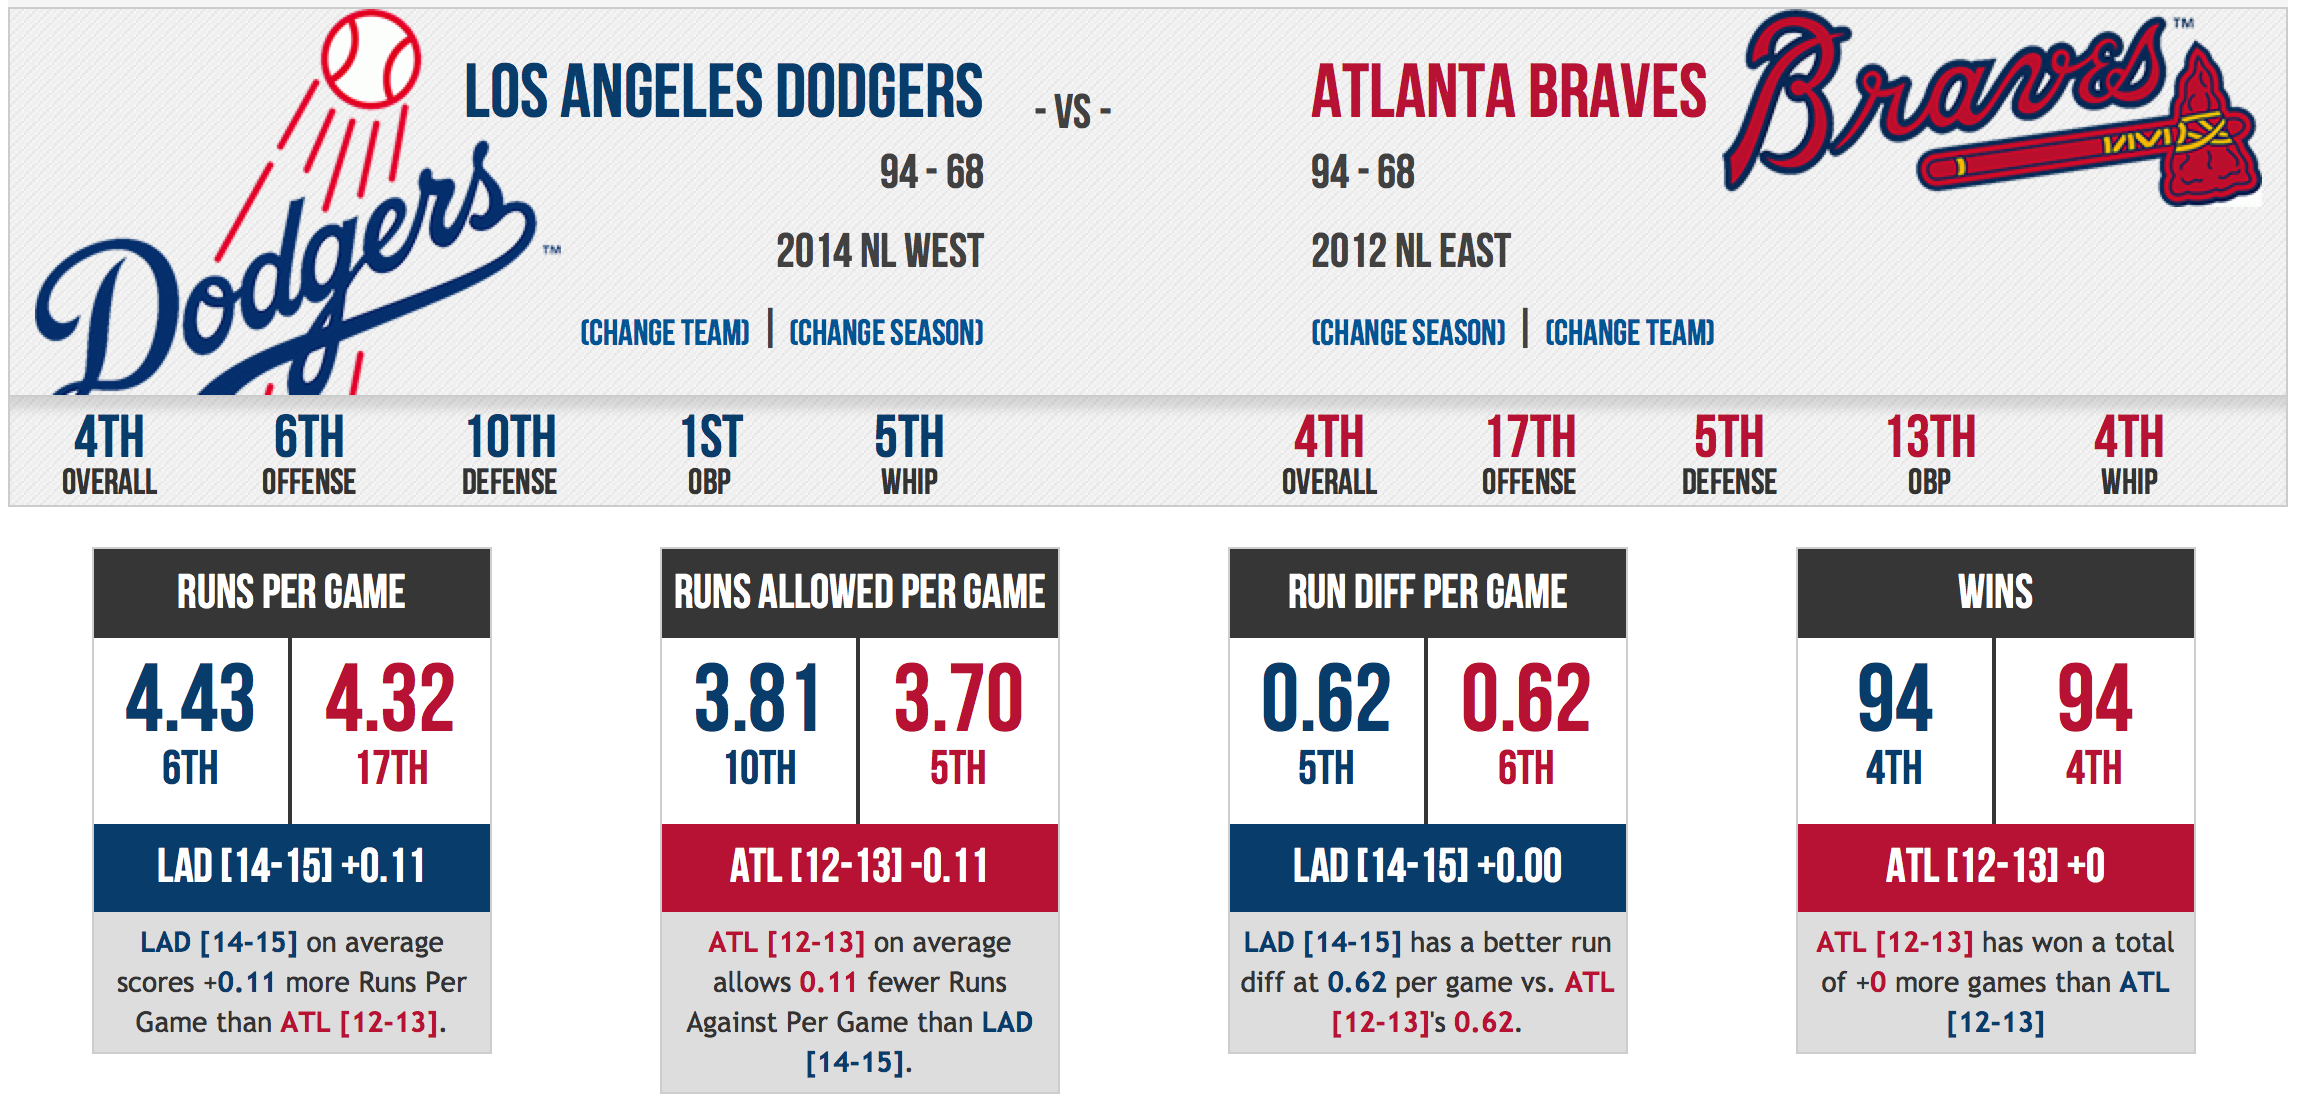
\includegraphics[width=0.7\textwidth]{dodgersbraves}
    \caption{Comparing 2012 Dodgers and 2014 Braves \href{http://www.sportingcharts.com/mlb/teams/matchup/243-los-angeles-dodgers-2014-vs-239-atlanta-braves-2012/}{source}}
\end{figure}

This shows that we are on the right track. Now, we check our similarity scores using visualization. We graph our sabremetric values and investigate any groupings. From there, we then derive some form of similarity and compare these clusters with the the similarity scores obtained from our algorithm.

\textit{Note: team scores accounts for the average, so when we transition to player comparisons, it'll be slightly different. For teams, because the statistics of the entire team is what is important, having 2 aces (Dodgers) vs. 4 good starters (Braves) resulted in the same score. In the case of individual players, we go by season statistics. However, we can take a step further than teams (single data point) by isolating each individual year as a separate data point and querying across those years, rather than taking the average. This will give us a better result.}

\section{Visualization} %%%%%%%%%%
We then visualized our results (both sabremetrics and the similarities results). Specifically, we took our sabremetric results and applied similarities in groupings, and the compared them to our derived numerical similarity results.

\subsection{Mondrian} %%%%%%
I applied my similarity results to Mondrian and looked at the associations or patterns.
\begin{figure}[H] 
  \begin{subfigure}[b]{0.5\linewidth}
    \centering
    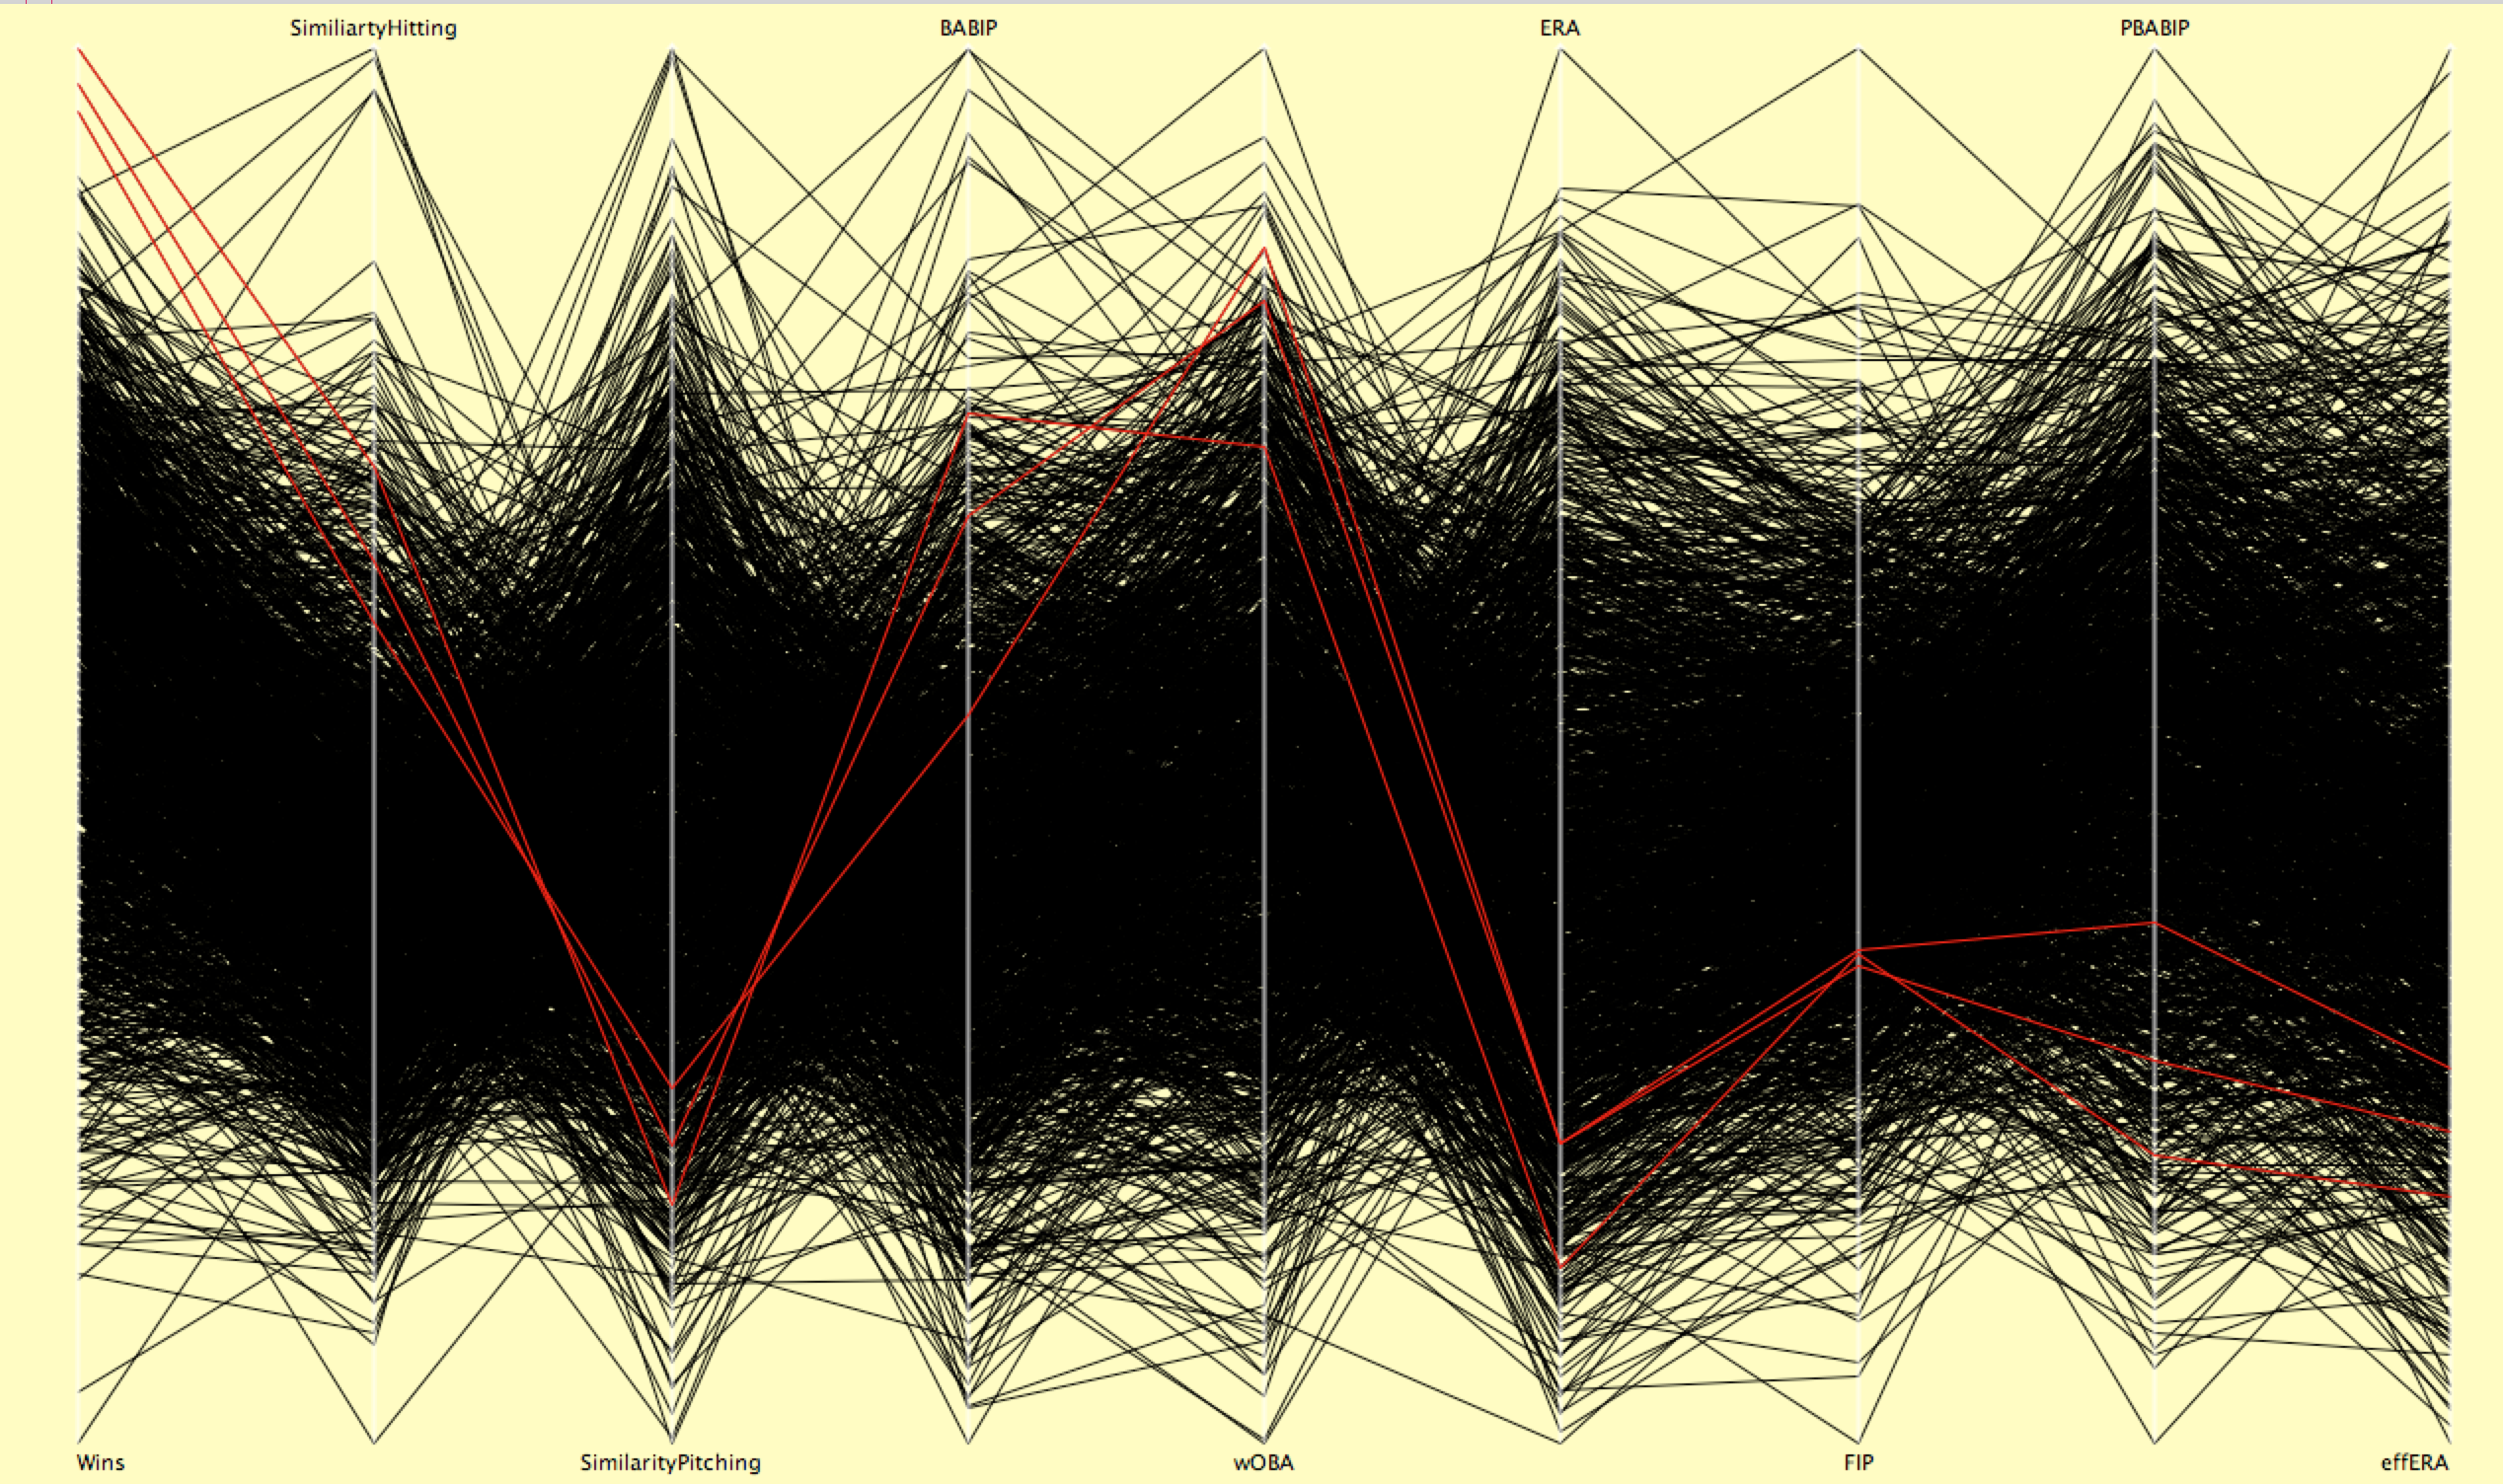
\includegraphics[width=0.9\linewidth]{h1} 
    \caption{Mondrian high wins} 
    \label{fig5:a} 
    \vspace{4ex}
  \end{subfigure}%% 
  \begin{subfigure}[b]{0.5\linewidth}
    \centering
    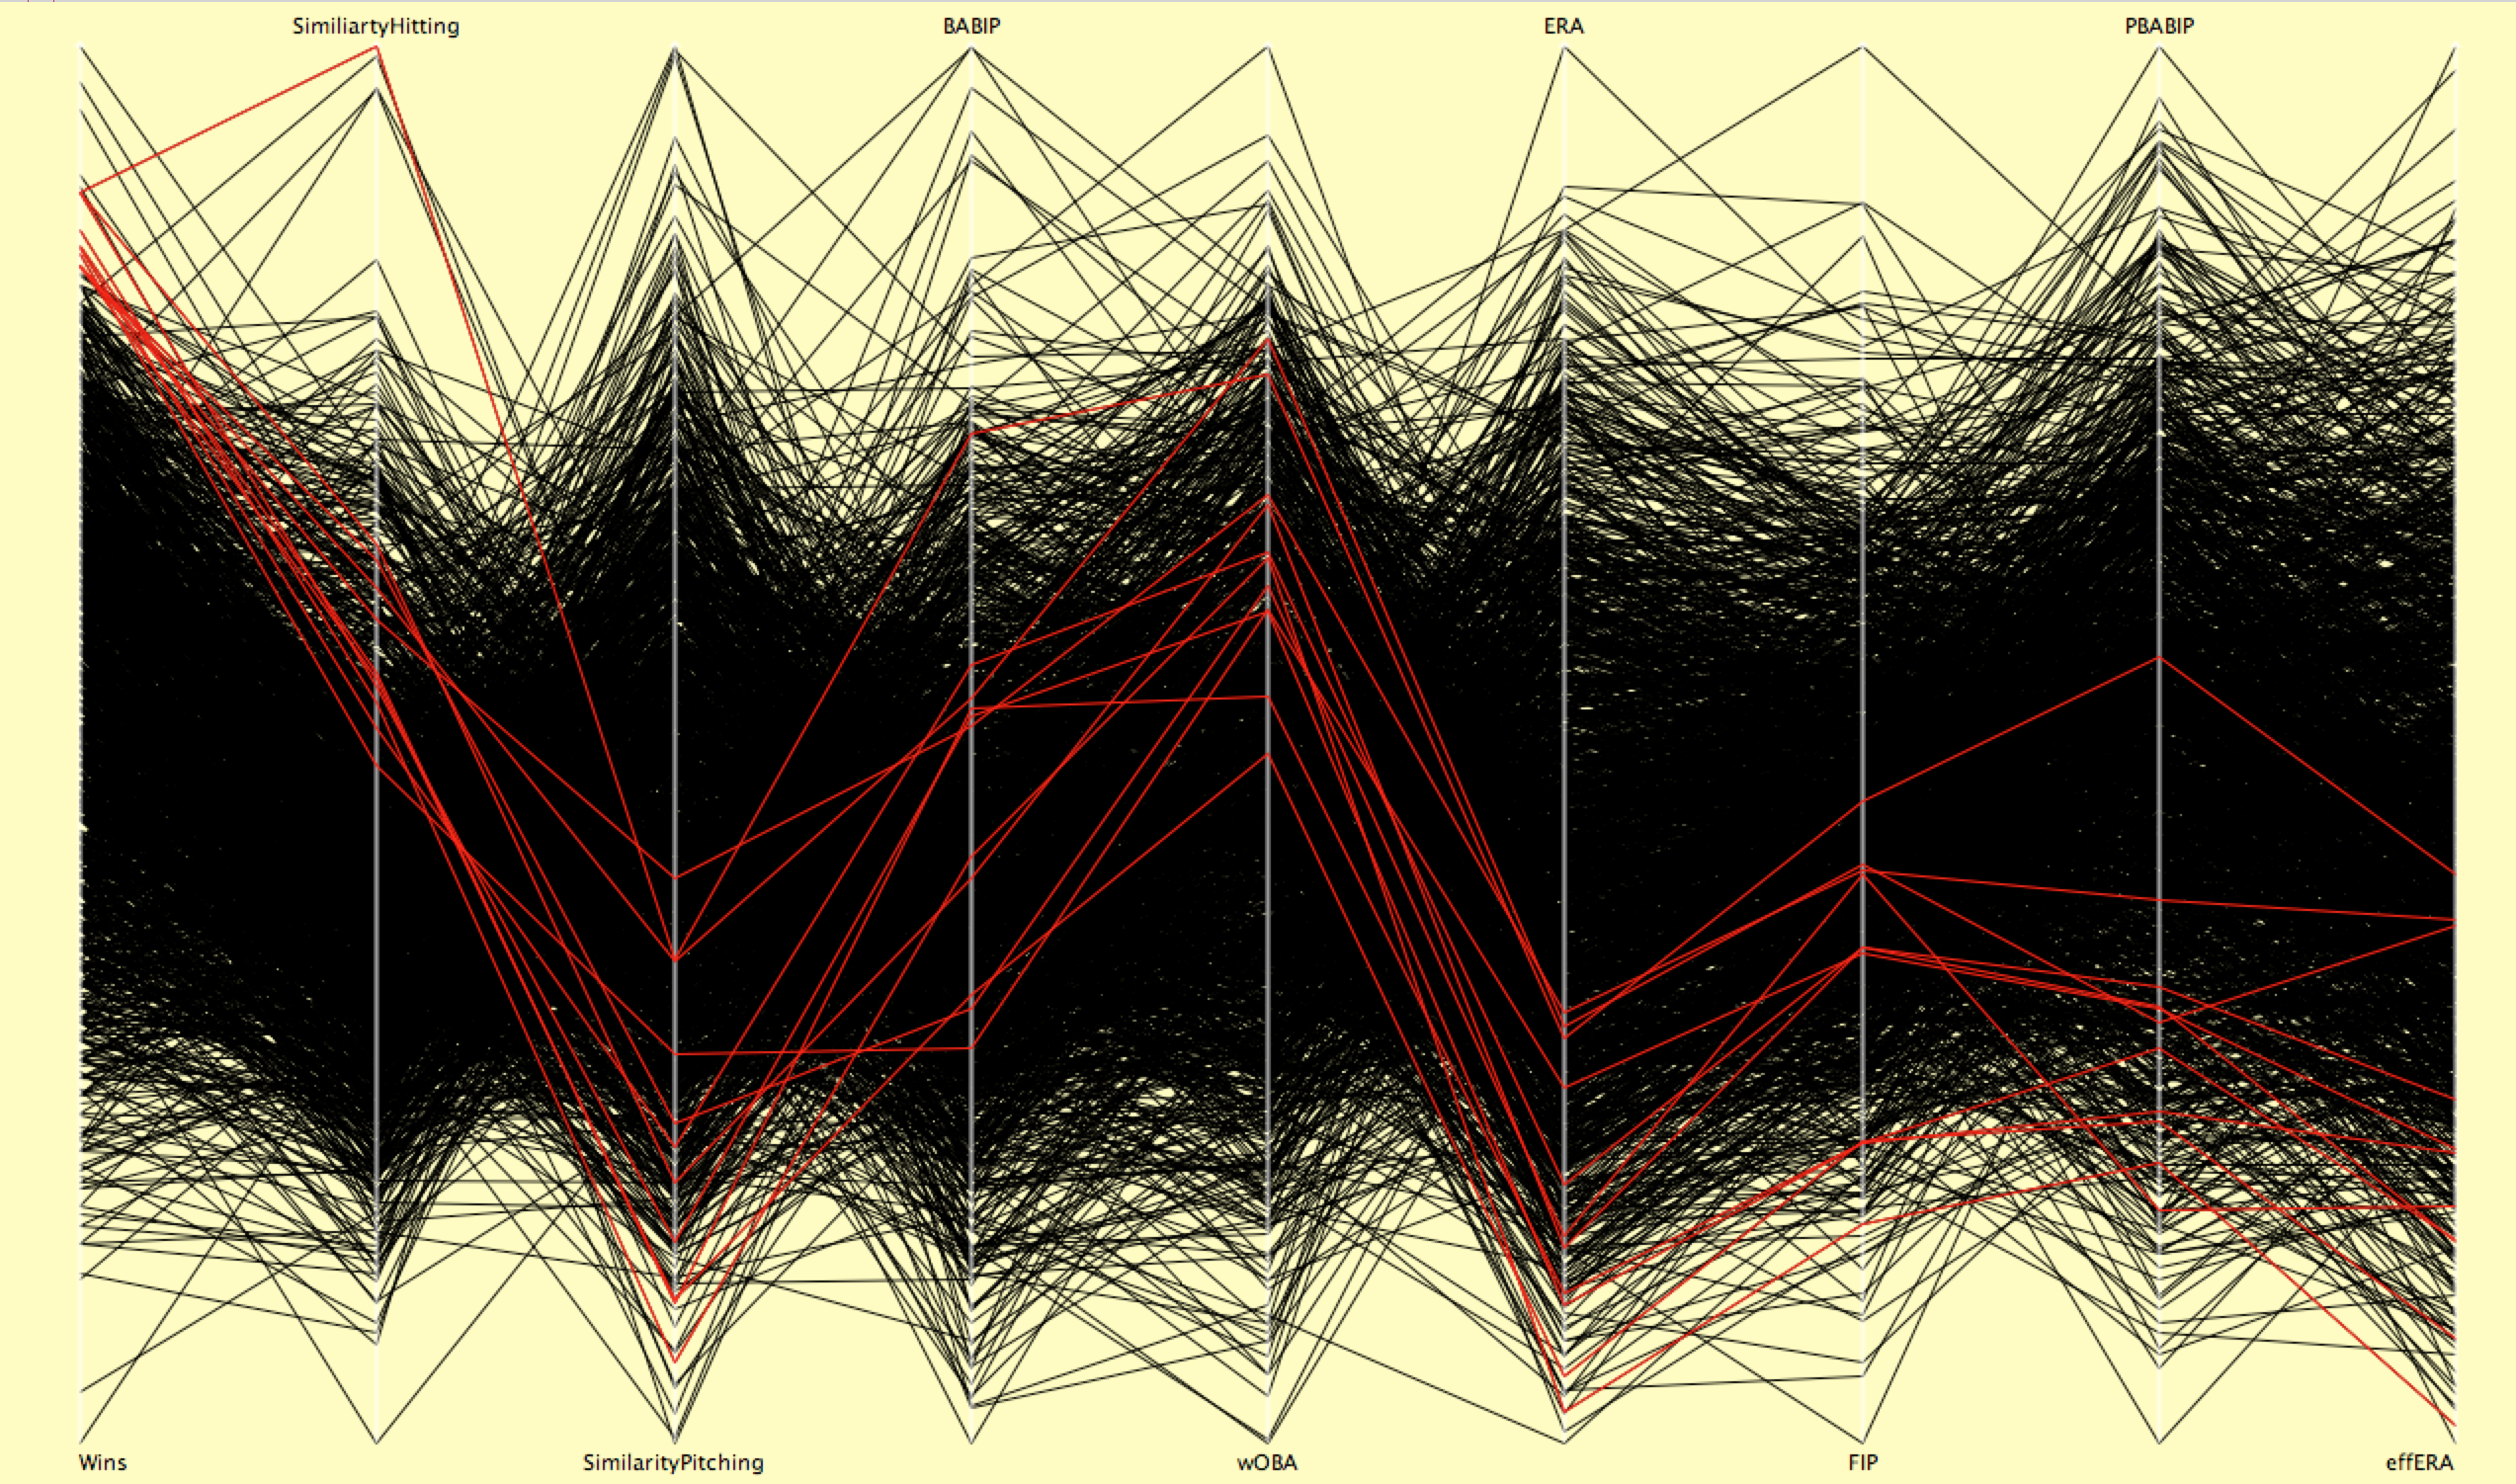
\includegraphics[width=0.9\linewidth]{h2} 
    \caption{Mondrian high wins} 
    \label{fig5:b} 
    \vspace{4ex}
  \end{subfigure} 
  \begin{subfigure}[b]{0.5\linewidth}
    \centering
    \includegraphics[width=0.9\linewidth]{h3} 
    \caption{Mondrian median wins} 
    \label{fig5:c} 
  \end{subfigure}%%
  \begin{subfigure}[b]{0.5\linewidth}
    \centering
    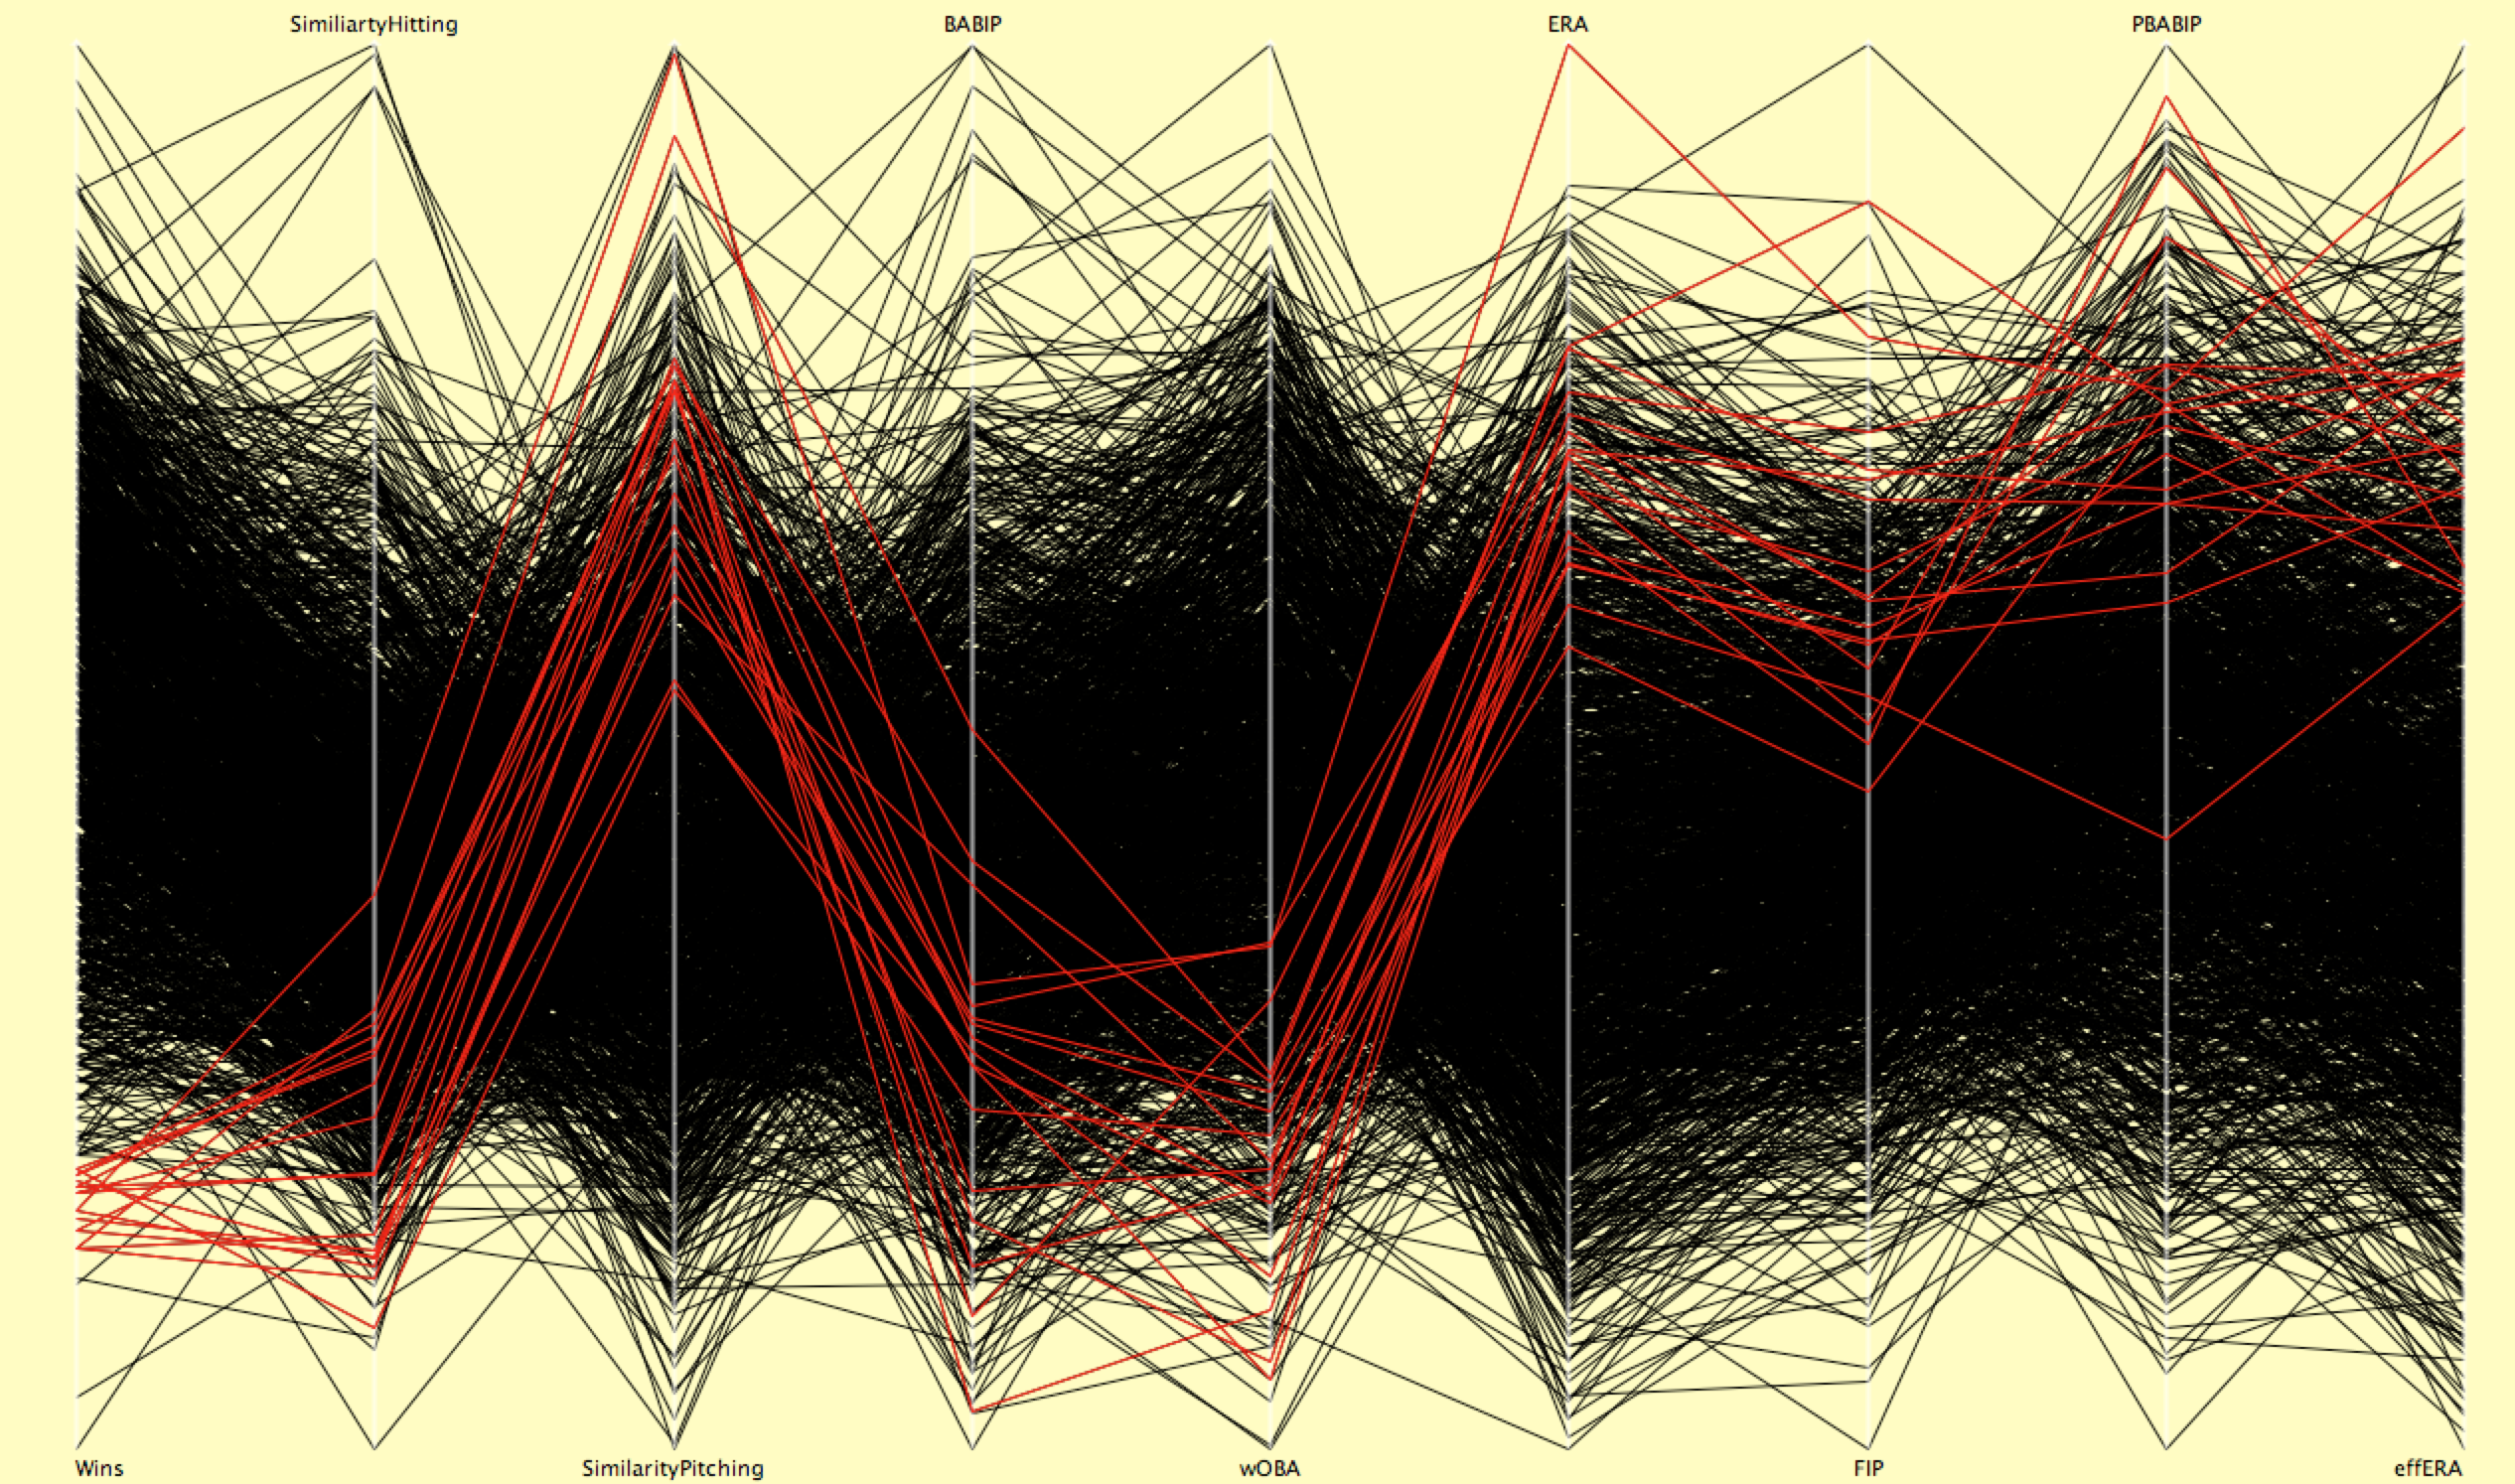
\includegraphics[width=0.9\linewidth]{h4} 
    \caption{Mondrian low wins} 
    \label{fig5:d} 
  \end{subfigure} 
  \caption{Similarity scores visualized on Mondrian}
  \label{fig5} 
\end{figure}

The map from left to right reads -- Wins, similarity hitting scores, similarity pitching scores, BABIP, wOBA, ERA, FIP, PBABIP, and effERA. You will notice that like those with high wins in the season standings, they share very similar offensive statistics and pitching statistics. This is the same case for those with low wins in the season standings. It is interesting to note that the higher Wins teams tended to have a much better pitching score than batting score, suggesting the importance of pitching over batting. This was not apparent in the lower Wins teams -- they had equally bad hitting and pitching. For those in the middle of the pack, around the average, they're offensive and pitching statistics were varied.

\begin{figure}[H] 
  \begin{subfigure}[b]{0.5\linewidth}
    \centering
    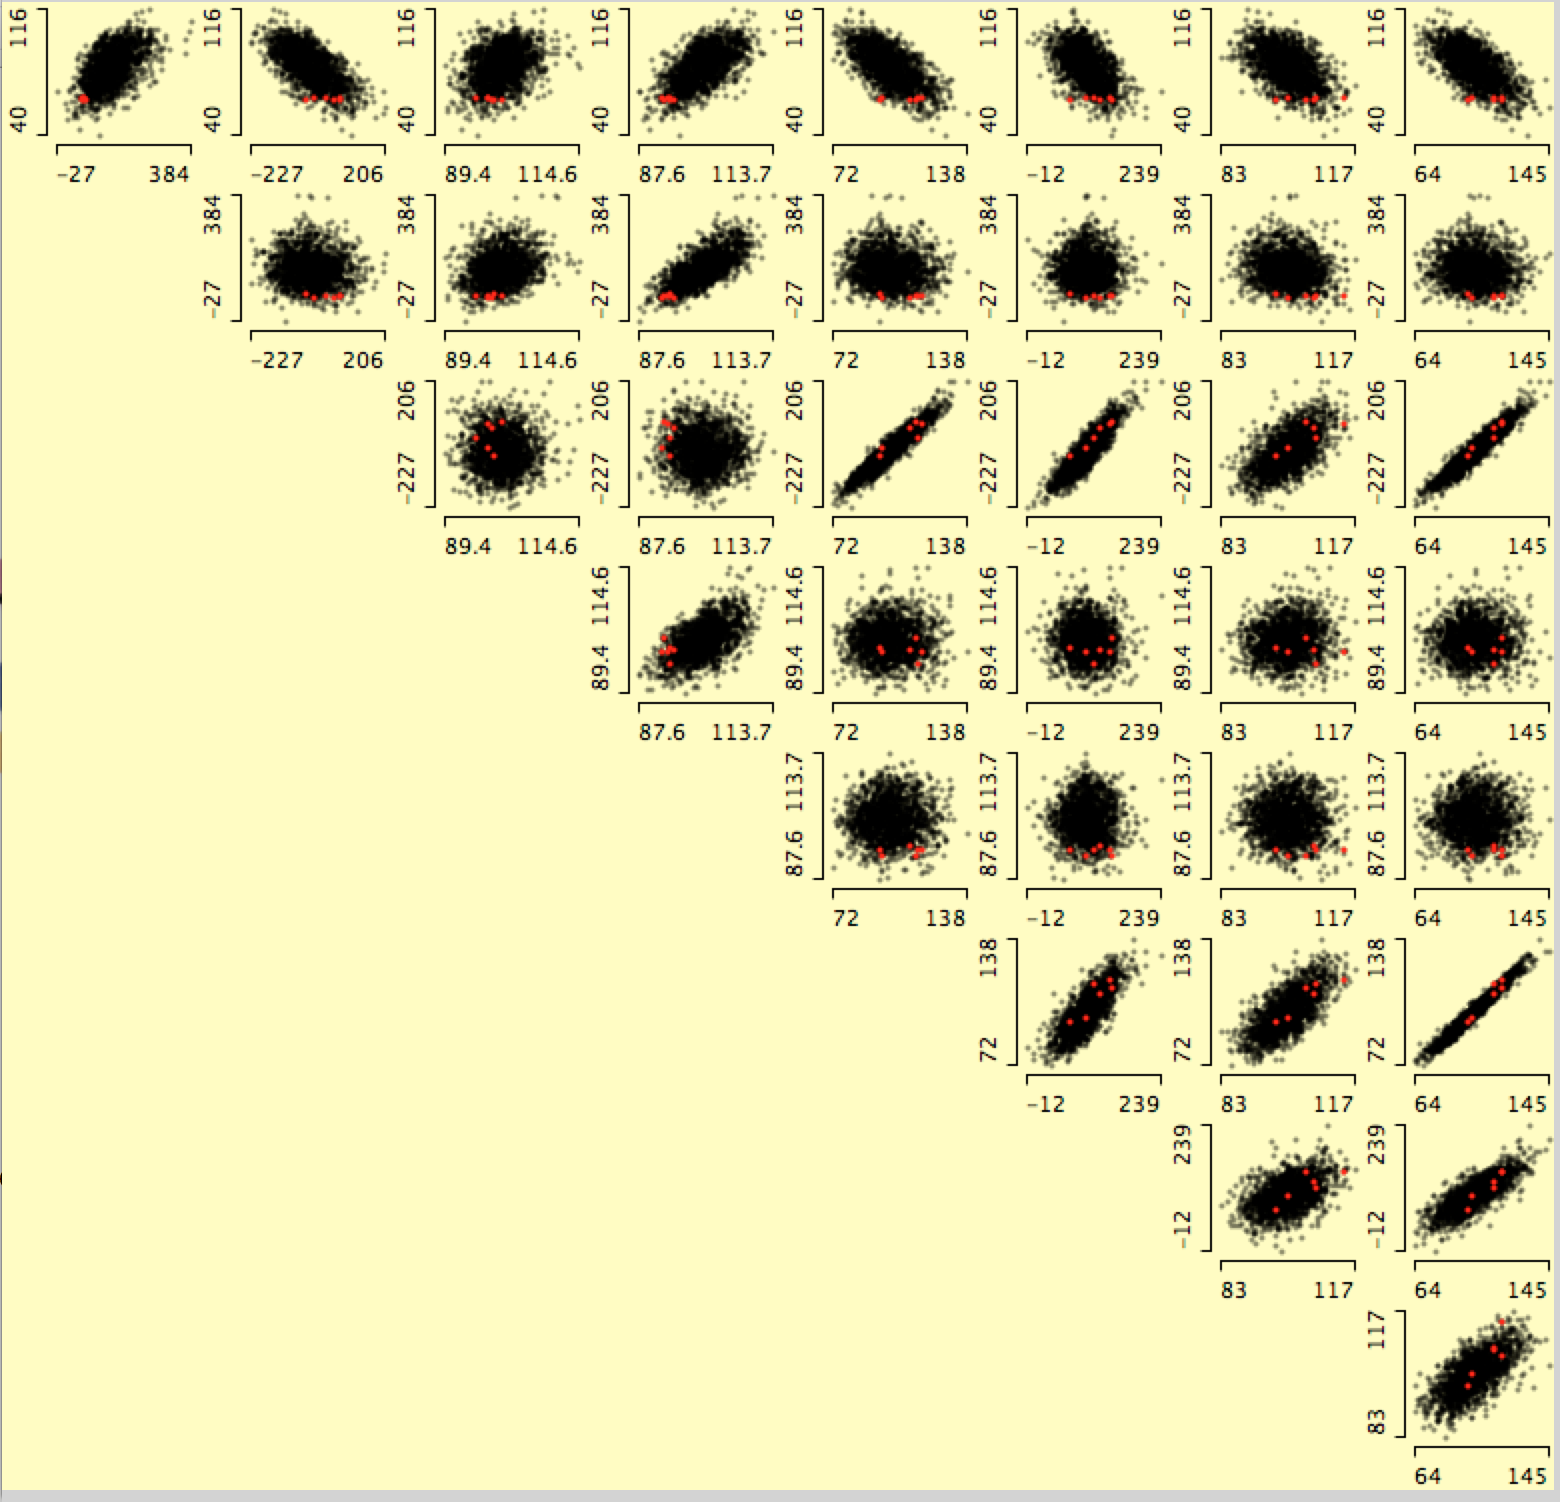
\includegraphics[width=0.7\linewidth]{h5} 
    \captionsetup{justification=centering}
    \label{fig2:a} 
    \vspace{4ex}
  \end{subfigure}%% 
  \begin{subfigure}[b]{0.5\linewidth}
    \centering
    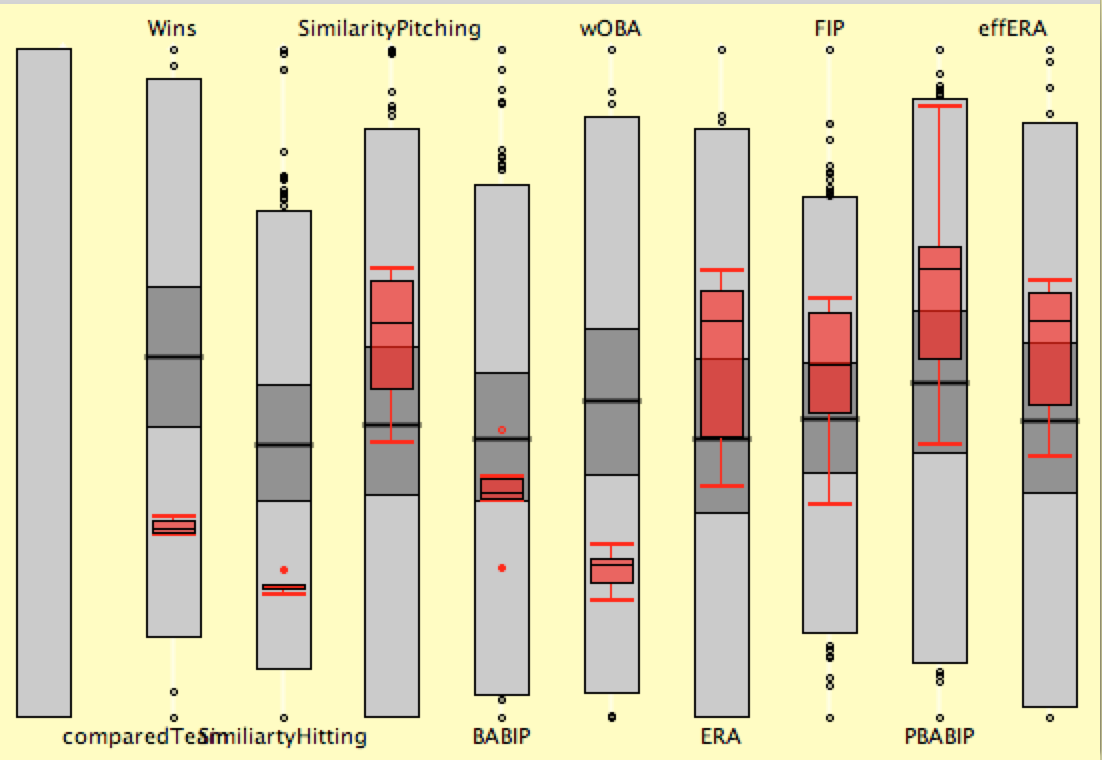
\includegraphics[width=0.9\linewidth]{h6} 
    \captionsetup{justification=centering}
    \label{fig2:b} 
    \vspace{4ex}
  \end{subfigure} 
  \caption{2014 Results in various binnings. Note both the median or average wins had a very large distribution of the other categories}
\end{figure}

If we take a closer look and examine the offensive stats in relation to the pitching stats and similarity stats, you will notice a relatively week association, but nevertheless an association.

\begin{figure}[H] 
  \begin{subfigure}[b]{0.5\linewidth}
    \centering
    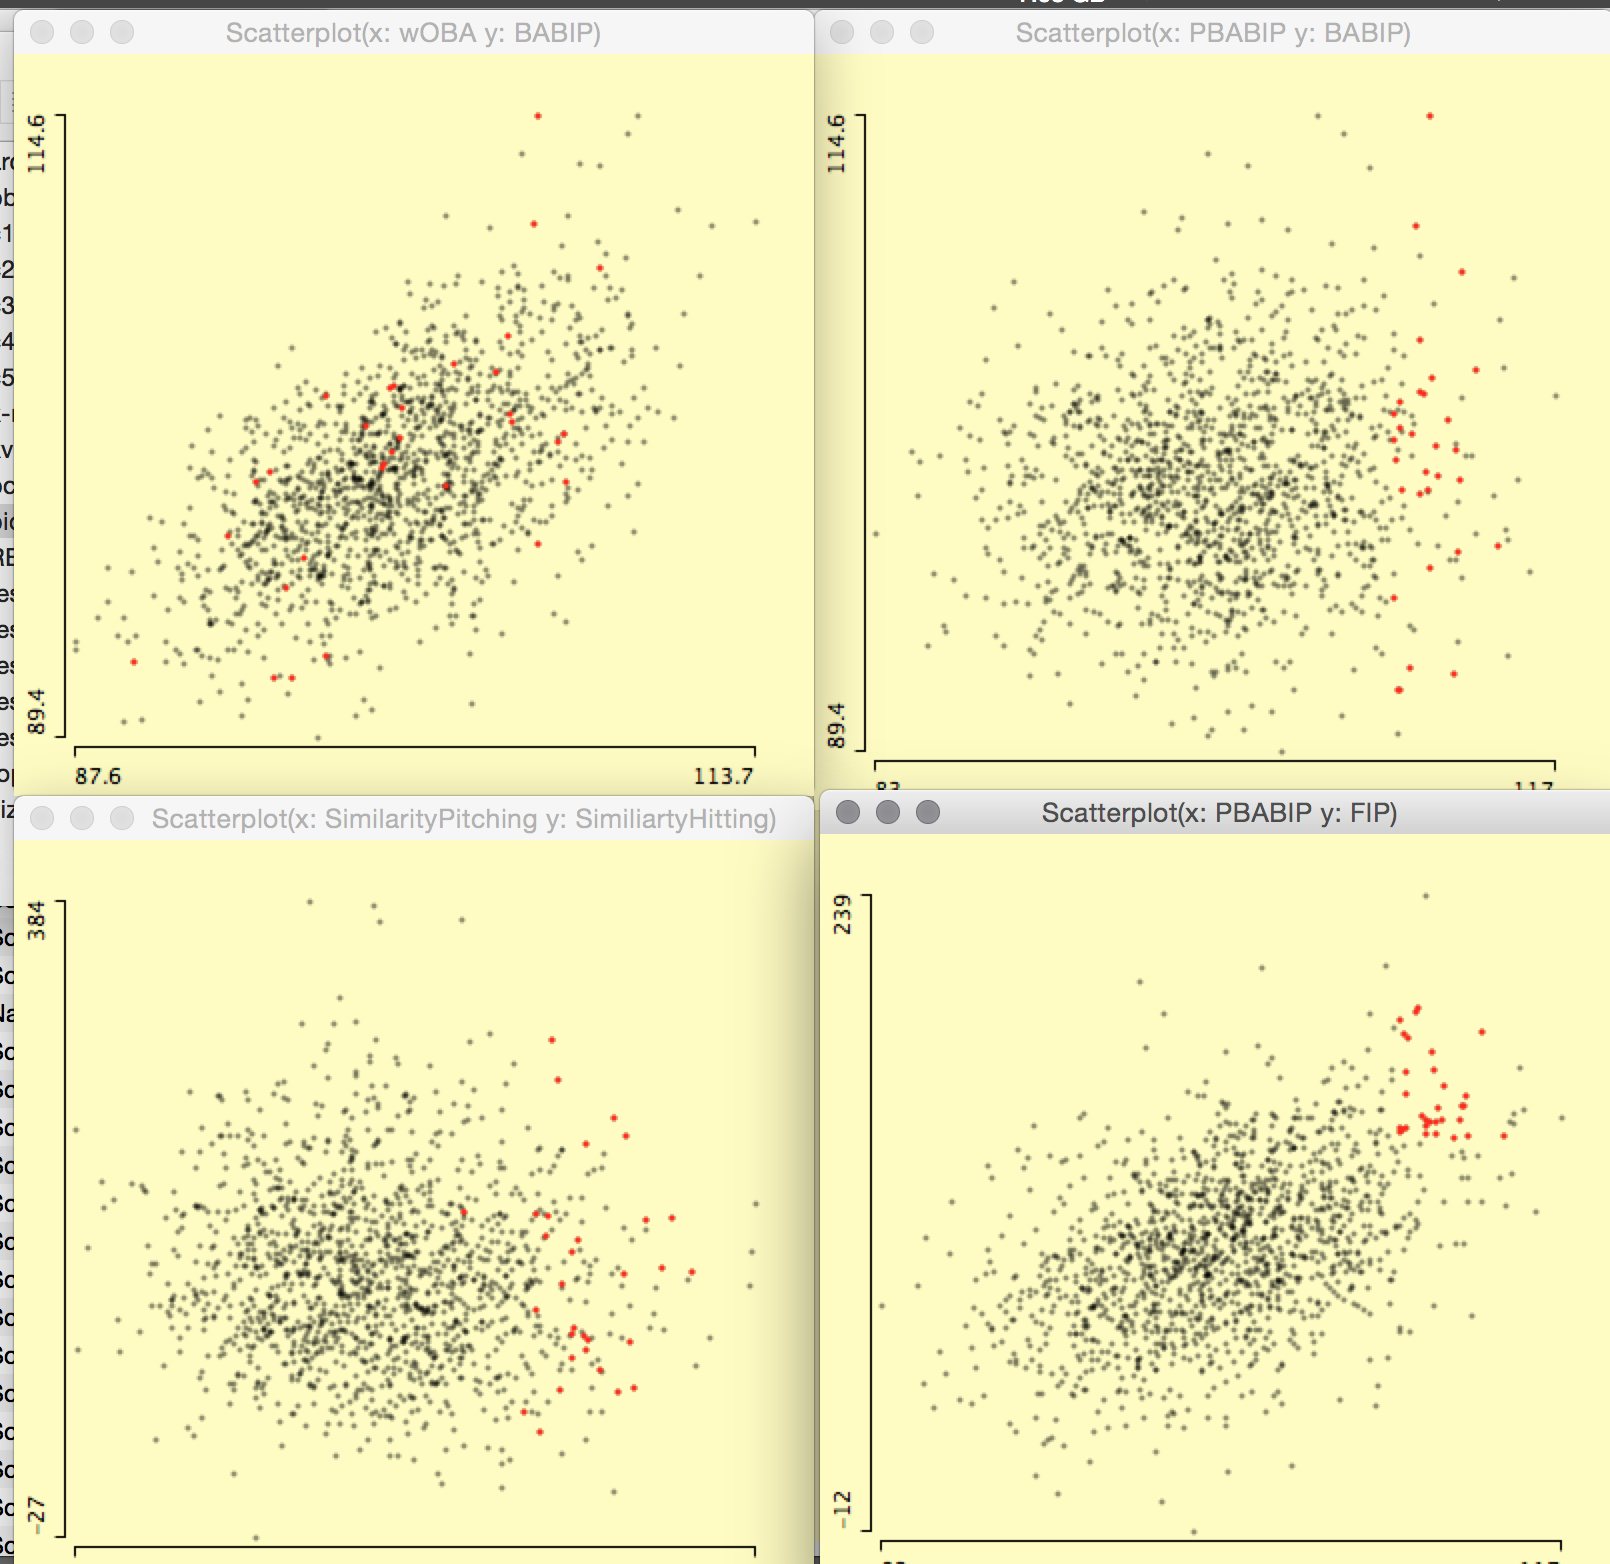
\includegraphics[width=0.9\linewidth]{m1} 
    \caption{bad pitching} 
    \label{fig5:a} 
    \vspace{4ex}
  \end{subfigure}%% 
  \begin{subfigure}[b]{0.5\linewidth}
    \centering
    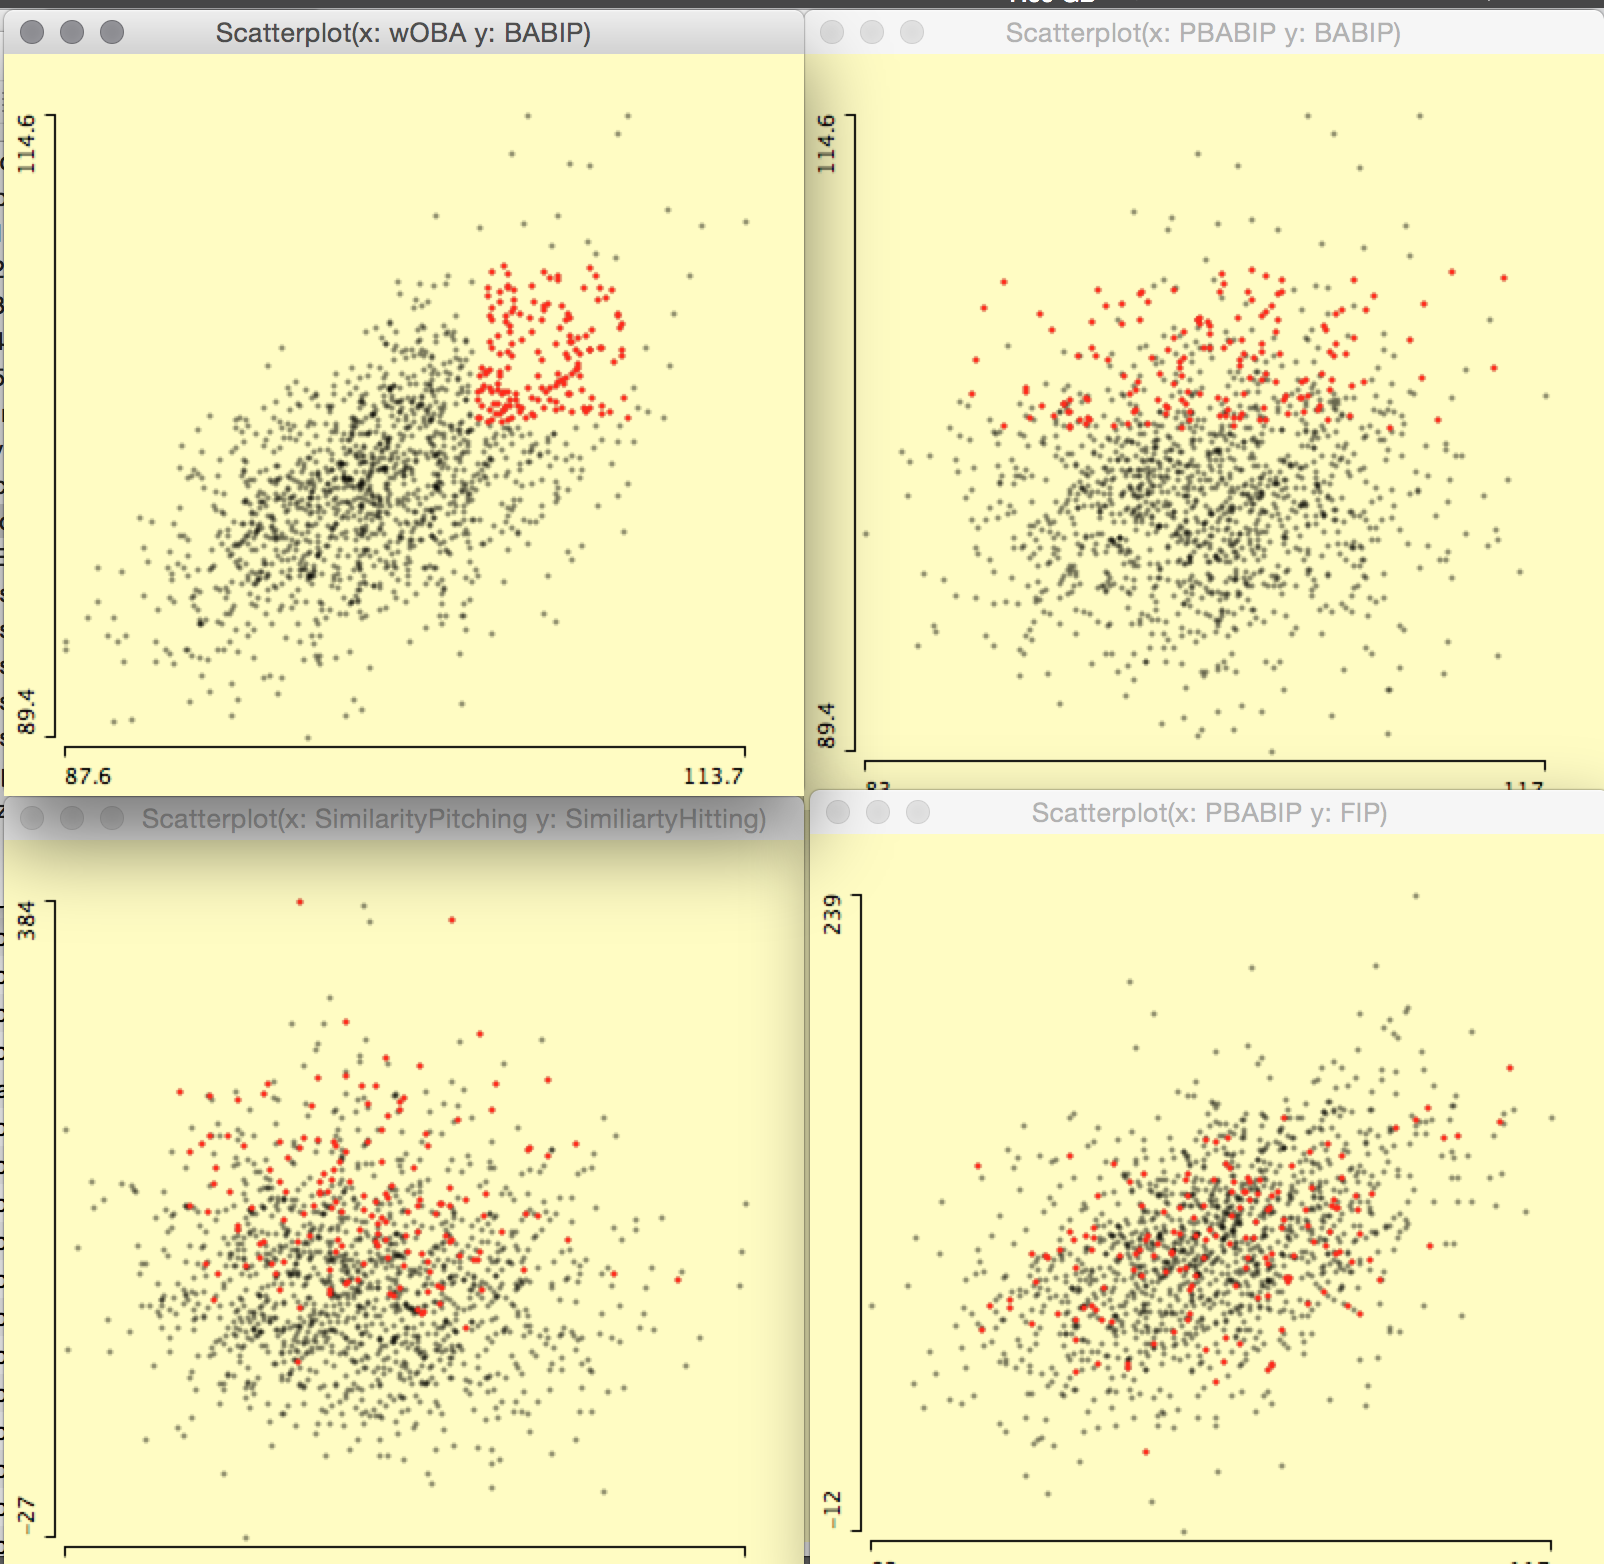
\includegraphics[width=0.9\linewidth]{m2} 
    \caption{good batting} 
    \label{fig5:b} 
    \vspace{4ex}
  \end{subfigure} 
  \begin{subfigure}[b]{0.5\linewidth}
    \centering
    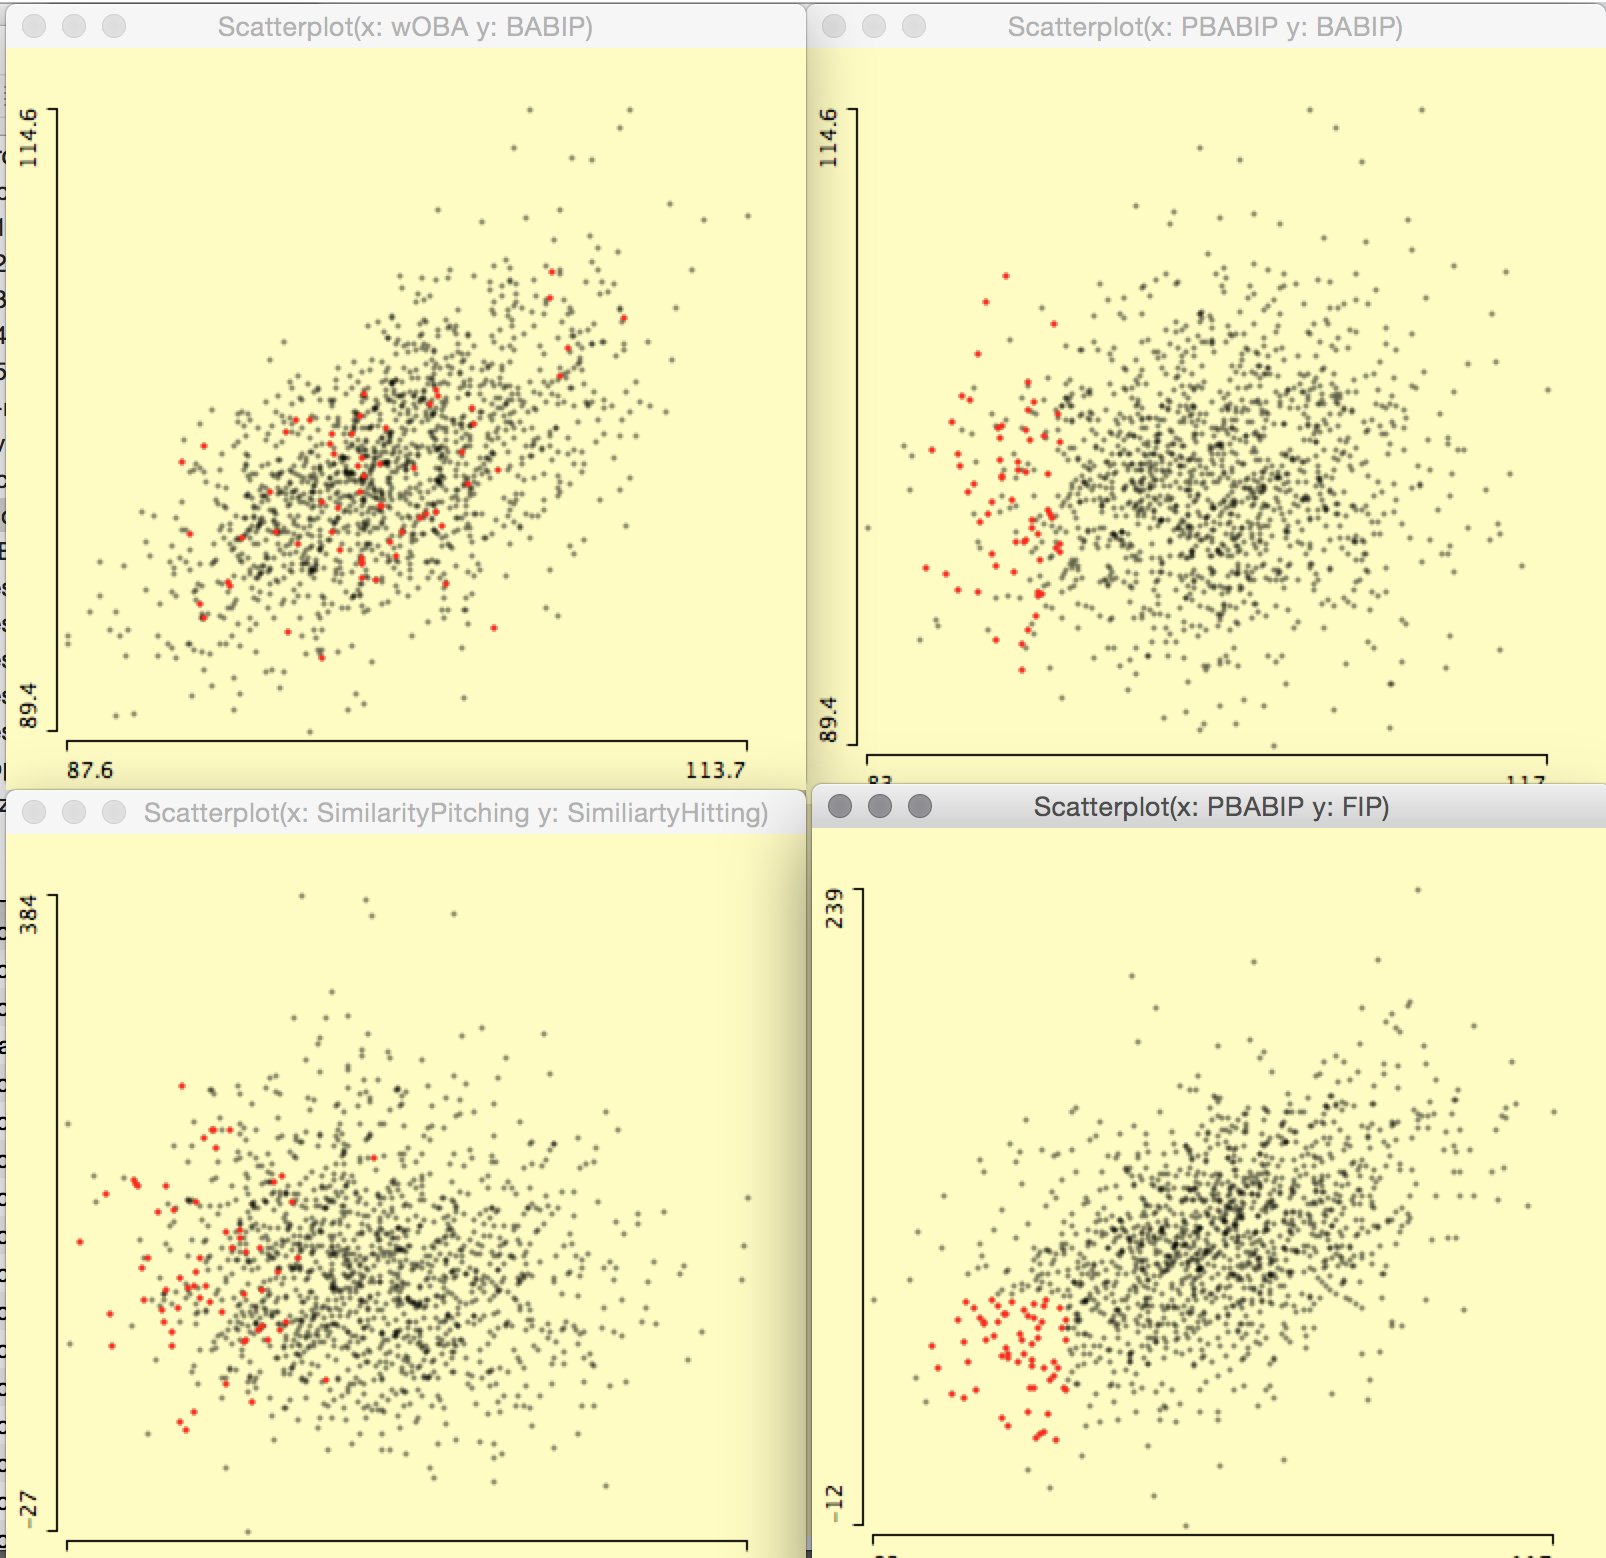
\includegraphics[width=0.9\linewidth]{m3} 
    \caption{good pitching} 
    \label{fig5:c} 
  \end{subfigure}%%
  \begin{subfigure}[b]{0.5\linewidth}
    \centering
    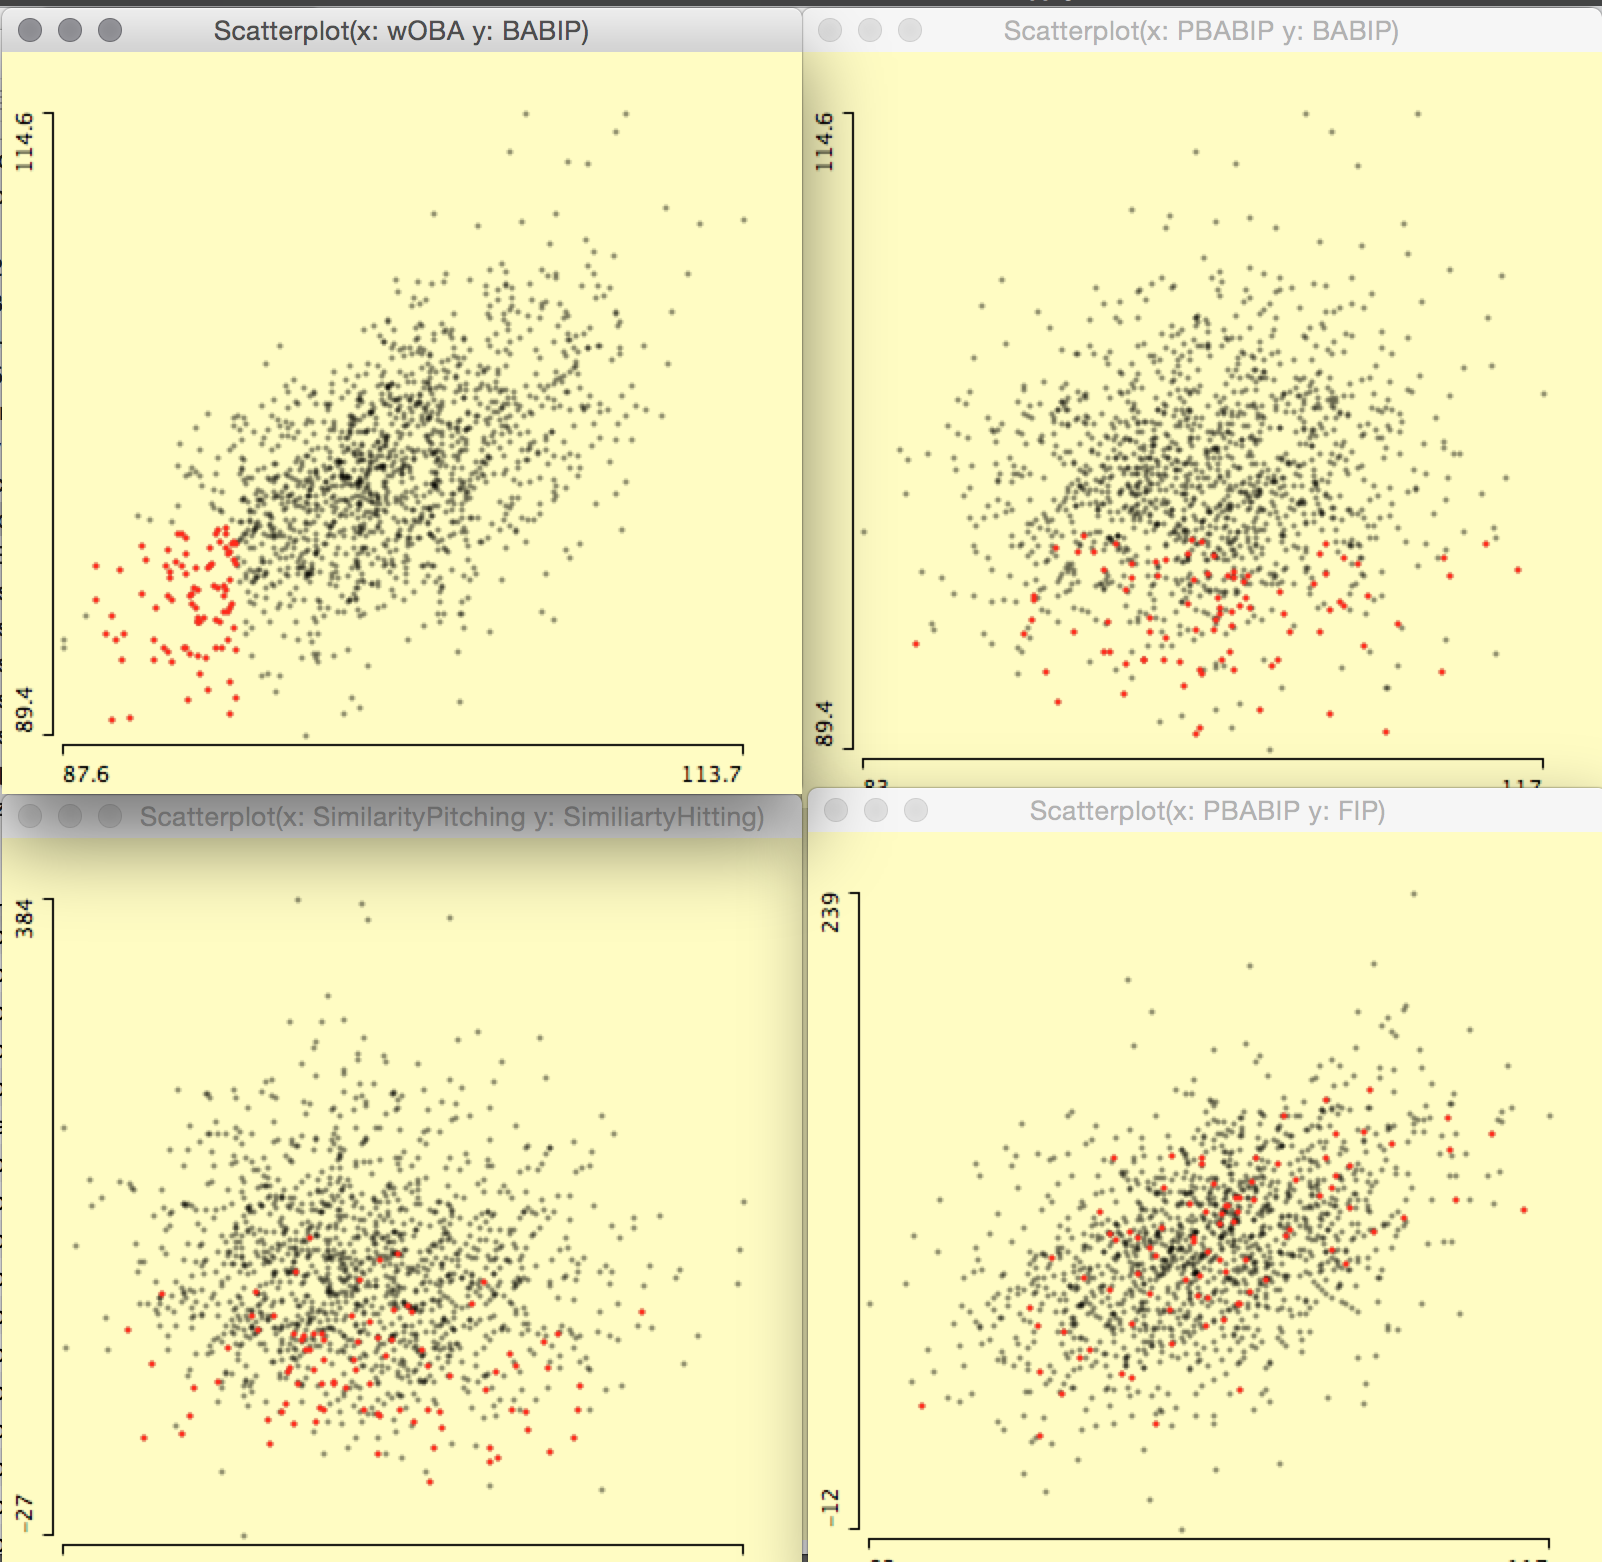
\includegraphics[width=0.9\linewidth]{m4} 
    \caption{poor batting} 
    \label{fig5:d} 
  \end{subfigure} 
  \caption{Similarity scores visualized on Mondrian}
  \label{fig50} 
\end{figure}

\noindent where in each subfigure in figure \ref{fig50} has uniquely
\begin{itemize}
	\item top left - BABIP vs. wOBA
    \item top right - BABIP vs. PBABIP
   	\item bottom left - SimilarityHitting vs.SimilarityPitching
    \item bottom right - FIP vs. PBABIP
\end{itemize}

\noindent and remember that 100 is the norm, relative to the league average. For pitching, it is generally under 100 that performance is above league average, while for batting it is generally above 100 that performance is above league average. For similarity scores, 

\begin{figure}[H] 
  \begin{subfigure}[b]{0.5\linewidth}
    \centering
    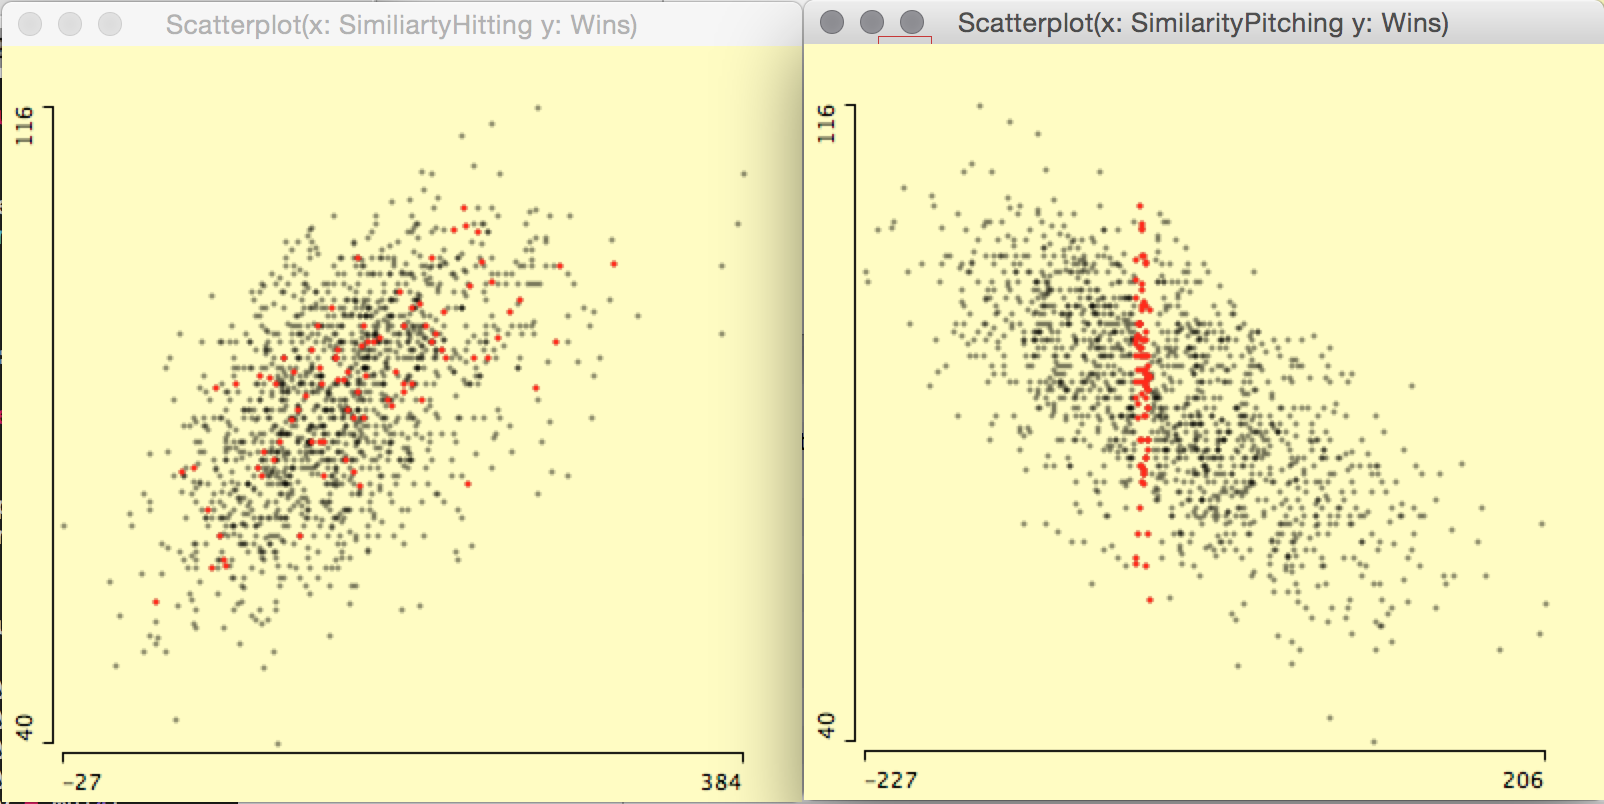
\includegraphics[width=0.9\linewidth]{similarity} 
    \captionsetup{justification=centering}
    \caption{Showing 1 to 1 independency between hitting and pitching scores}
    \label{fig2:a} 
    \vspace{4ex}
  \end{subfigure}%% 
  \begin{subfigure}[b]{0.5\linewidth}
    \centering
    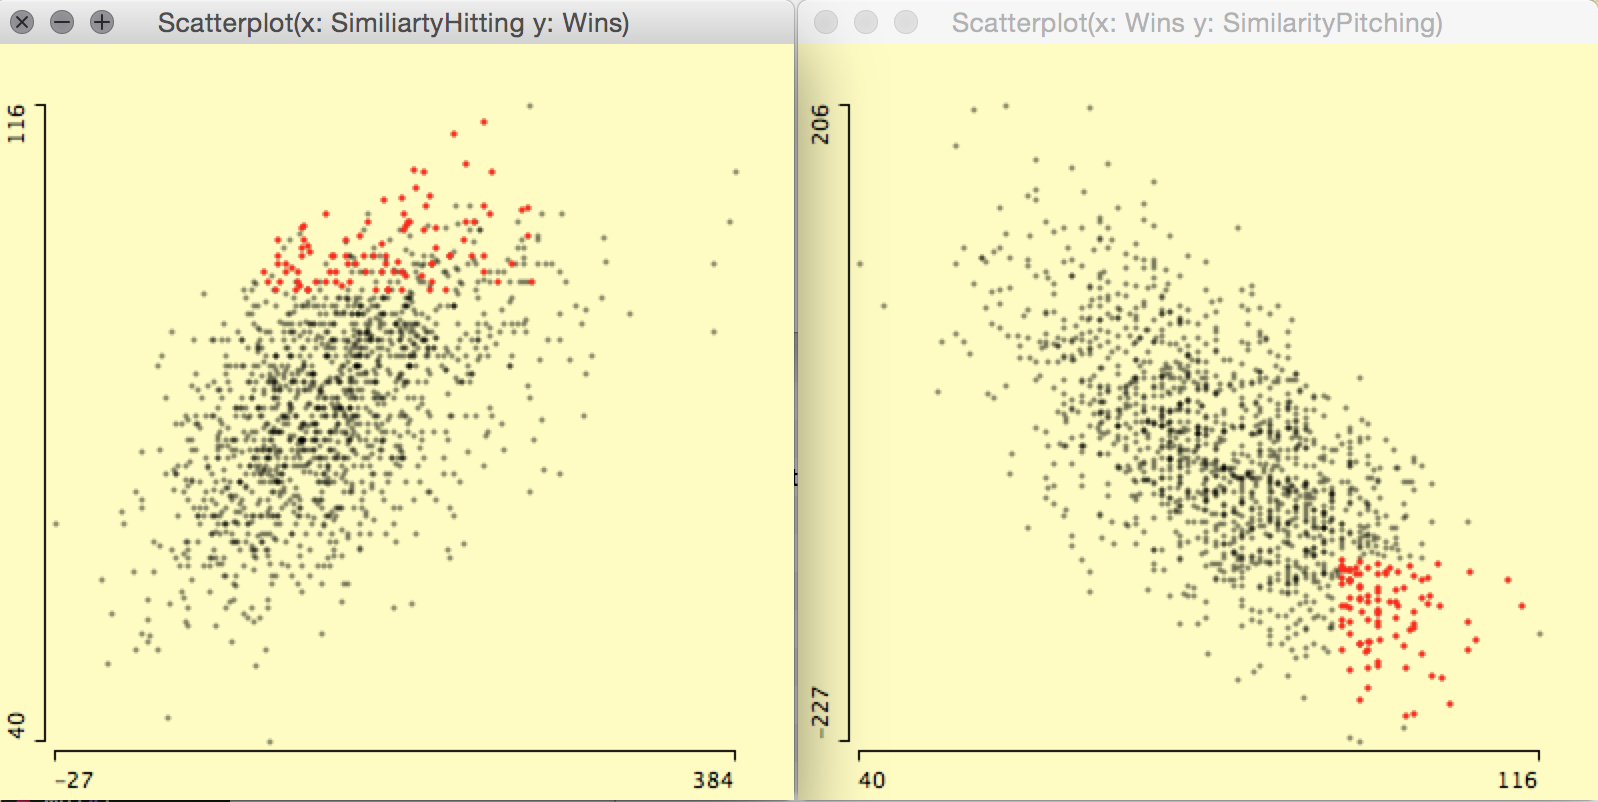
\includegraphics[width=0.9\linewidth]{similarity2} 
    \captionsetup{justification=centering}
    \caption{Showing commonalities between scores and wins}
    \label{fig2:b} 
    \vspace{4ex}
  \end{subfigure} 
  \caption{Similarity score to team wins}
\end{figure}

100 represents perfectly identical teams. We can see from our interpretations that more win teams tend to have higher batting similarity scores $(>100)$ and lower pitching similarity score $(<100)$. We also see that having nearly identical similarity scores in pitching or batting does not necessarily translate to batting or pitching similarity scores, which is a positive sign that these variables are independent. However, one can see that those teams with a good win-loss record tended to have high batting similarity scores, and low pitching similarity scores. It is important to see that although this is generally the trend, the spread is quite large, suggesting that teams can have a high win-loss record with good scores on one end. An example would be the 2015 St. Louis Cardinals with a 100 win record and a -156 pitching similarity score, but having an almost average 108 batting similarity score.

Looking at their \href{http://www.baseball-reference.com/teams/STL/2015.shtml}{traditional statistics} and \href{http://www.sportingcharts.com/mlb/teams/matchup/246-philadelphia-phillies-2015-vs-248-st.-louis-cardinals-2015/}{comparing} with the \href{http://www.baseball-reference.com/teams/PHI/2015.shtml}{2015 Philadelphia Phillies} (our reference), we see that the Cardinals had league average batting with league leading pitching. A quick comparison across multiple sites would confirm our findings.

\begin{figure}[H]
	\centering
	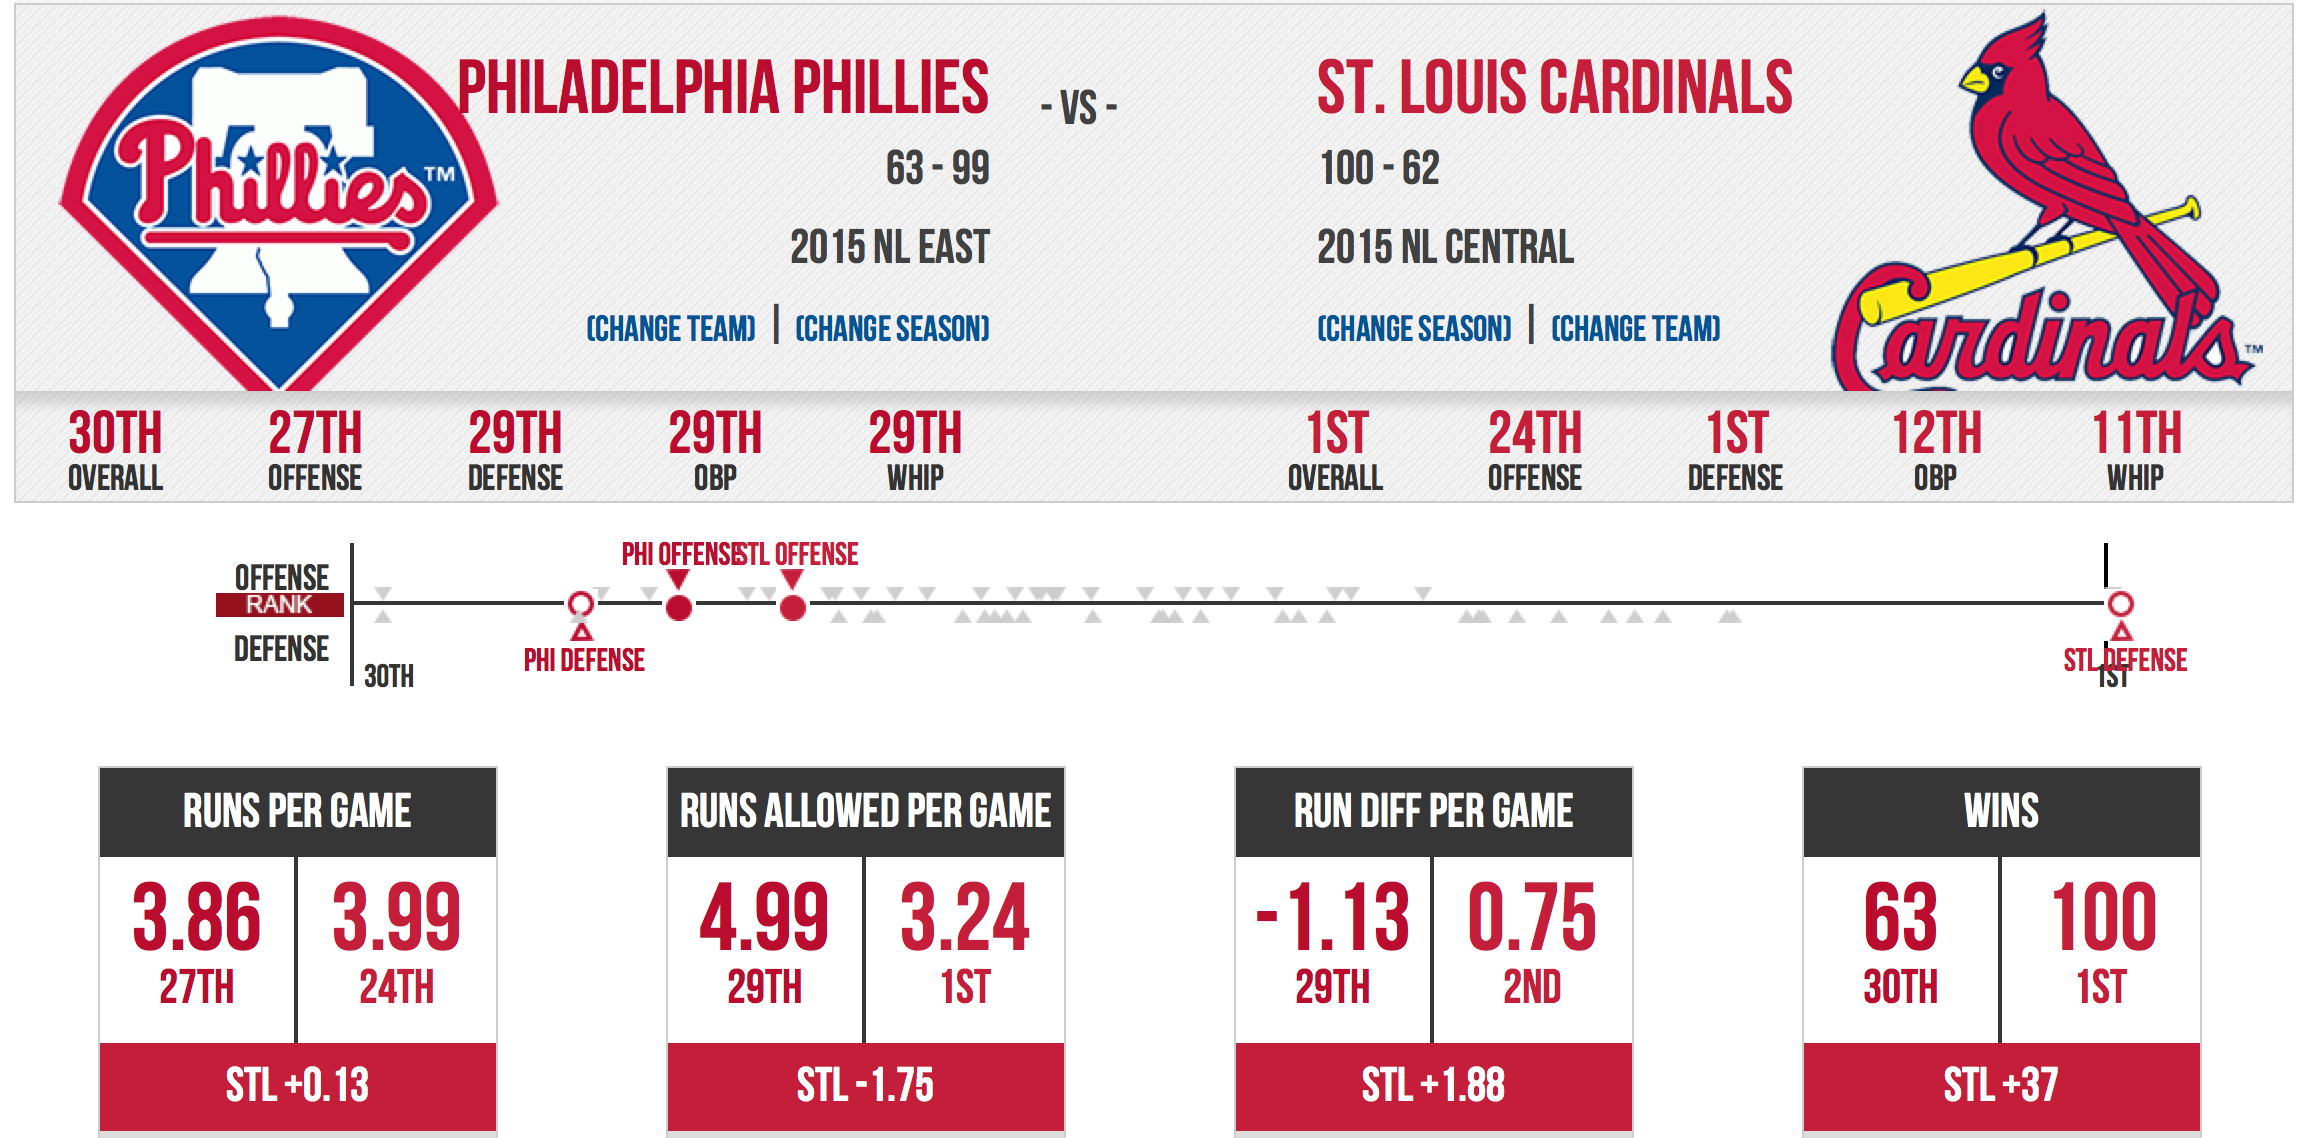
\includegraphics[width=0.7\textwidth]{infograph}
\end{figure}

\begin{figure}[H]
	\centering
	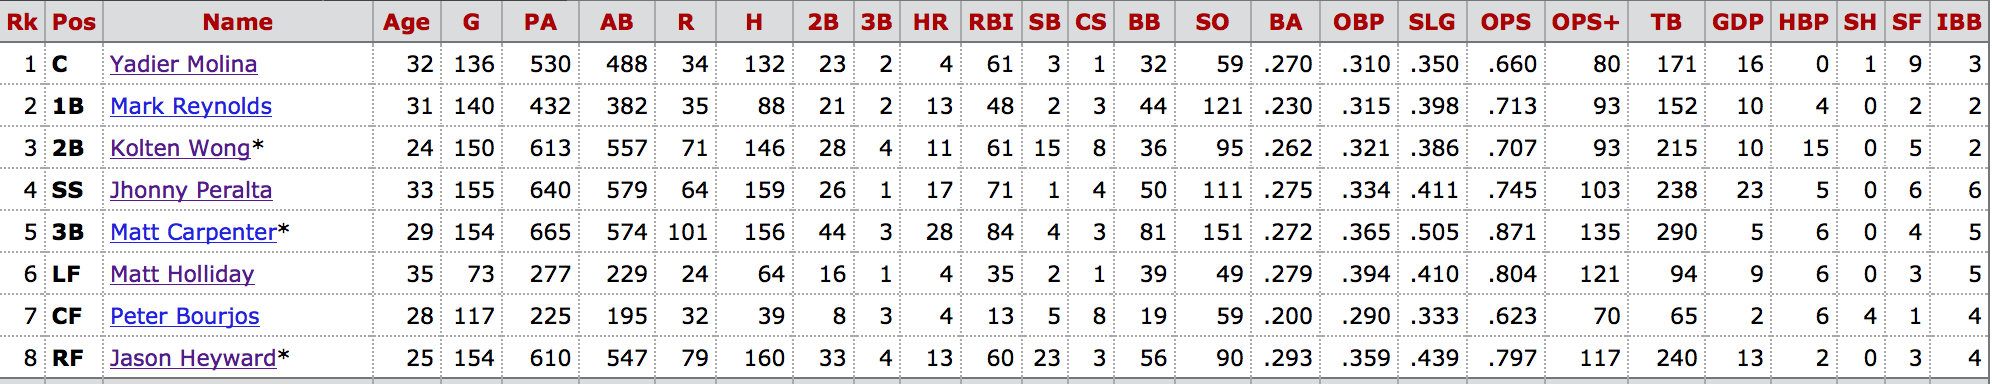
\includegraphics[width=0.9\textwidth]{infograph1}
    \caption{2015 Cardinals Batting}
\end{figure}

\begin{figure}[H]
	\centering
	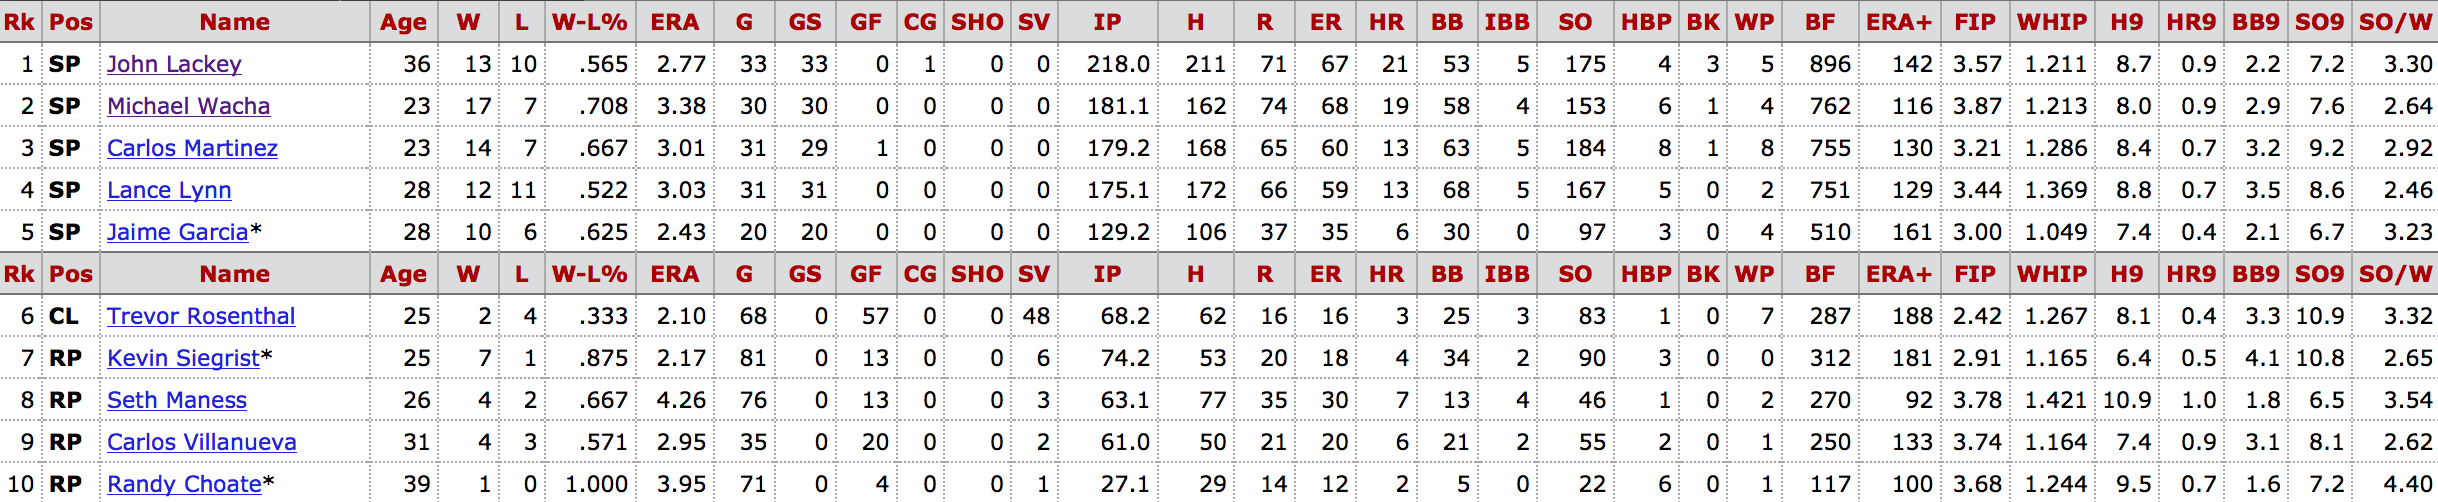
\includegraphics[width=0.9\textwidth]{infograph2}
    \caption{2015 Cardinals Pitching}
\end{figure}

\begin{figure}[H]
	\centering
	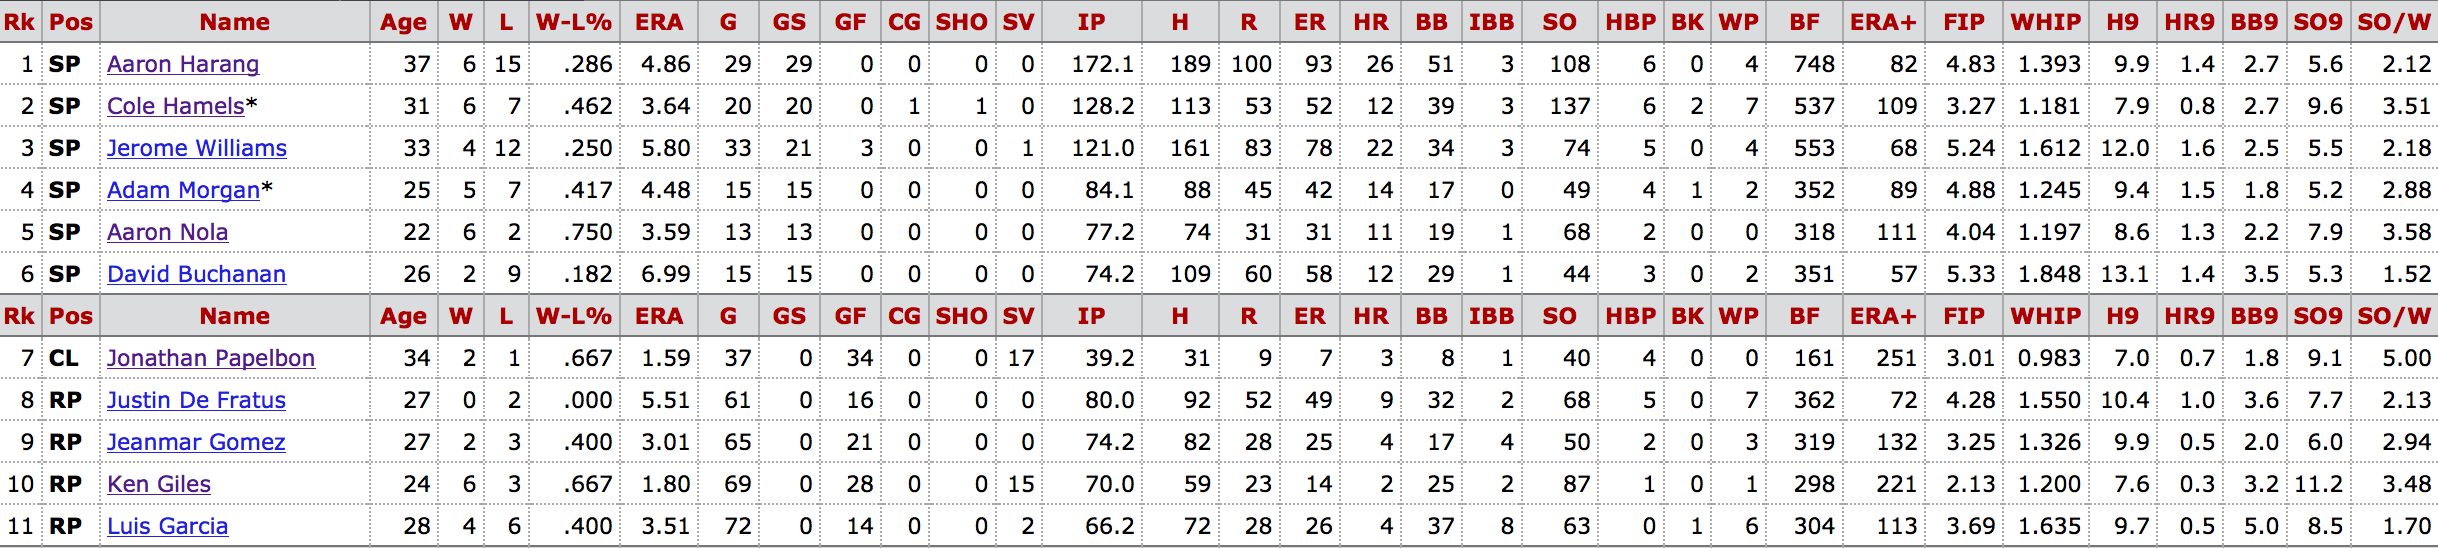
\includegraphics[width=0.9\textwidth]{infograph3}
    \caption{2015 Phillies Batting}
\end{figure}

\begin{figure}[H]
	\centering
	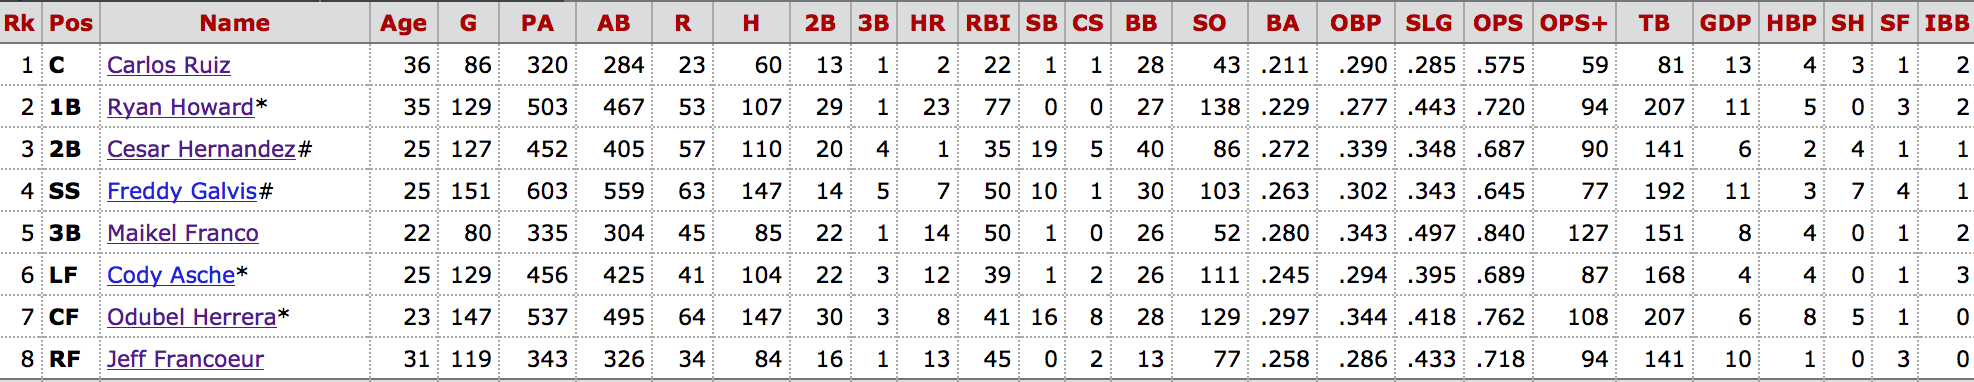
\includegraphics[width=0.9\textwidth]{infograph4}
    \caption{2015 Phillies Pitching}
\end{figure}


\subsubsection{Checking effectiveness of our effERA measurement}
To check how effective our effERA sabremetric was, we looked at the scatterplot of effERA and ERA.

\begin{figure}[H]
	\centering
	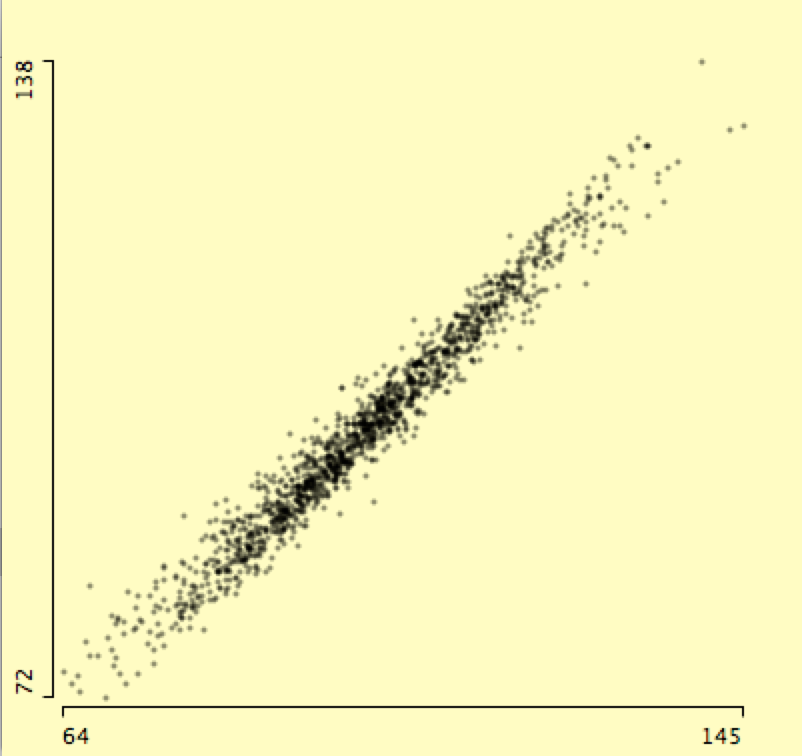
\includegraphics[width=0.5\textwidth]{effERA}
    \caption{effERA vs. ERA}
\end{figure}

The scatterplot shows a strong positive linear correlation between ERA and effERA, which is good and should suggest a reasonable statistic. What is interesting is that when we look at the extrema, we can see that the ends are rather less strongly correlated, or "opening up". This is interesting as this can suggest that really good or really bad ERAs put up by pitchers (and the team) could be due to other factors (ie. relief pitchers giving up runs left stranded by starters or fielders with realistically bad fielding, the opposite case for the two, or just being rather unlucky). The incorporation of SVs, CG, SHO, and FLD helps identify these cases. It seems that the effERA is a rather sufficient tool in analyzing true team ERA, and can be applied to individual pitchers in the future. The coefficients are rather arbitrary, and will need some adjustments later down the road.

\subsection{Paraview} %%%%%%

From here, we then looked into another visualization program, Paraview. Although our dataset is not time-dependent, given that each dataset is by individual year, we examine our team set results using a selection of tools.


\begin{figure}[H] 
  \begin{subfigure}[b]{0.5\linewidth}
    \centering
    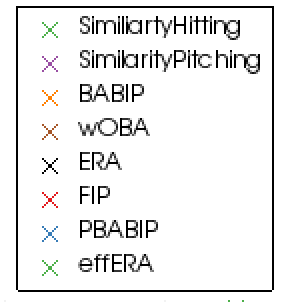
\includegraphics[width=0.6\linewidth]{winslegend} 
    \captionsetup{justification=centering}
    \label{fig2:a} 
    \vspace{4ex}
  \end{subfigure}%% 
  \begin{subfigure}[b]{0.5\linewidth}
    \centering
    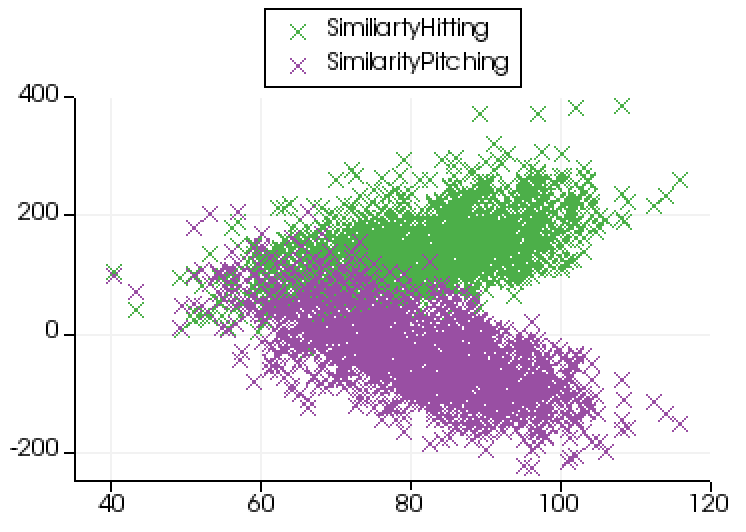
\includegraphics[width=0.9\linewidth]{wins1} 
    \captionsetup{justification=centering}
    \label{fig2:b} 
    \vspace{4ex}
  \end{subfigure} 
  \caption{Similarity score to team wins}
\end{figure}

We see the very clear association and (because these are numerical or quantitative), very clear correlation between similarity hitting and similarity pitching and team wins. Note that the correlation may not be as strong because of the relative spread of the data points along the regression fit.

\begin{figure}[H] 
  \begin{subfigure}[b]{0.5\linewidth}
    \centering
    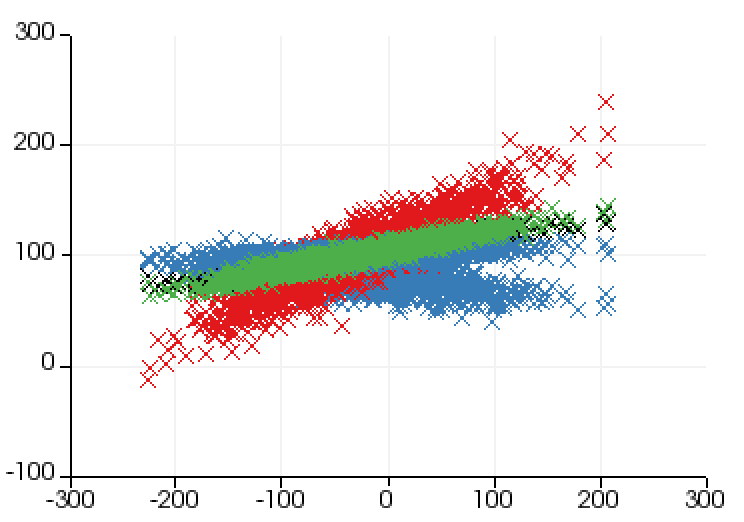
\includegraphics[width=0.9\linewidth]{similarpitch2} 
    \caption{Pitching metrics scaled} 
    \label{fig5:a} 
    \vspace{4ex}
  \end{subfigure}%% 
  \begin{subfigure}[b]{0.5\linewidth}
    \centering
    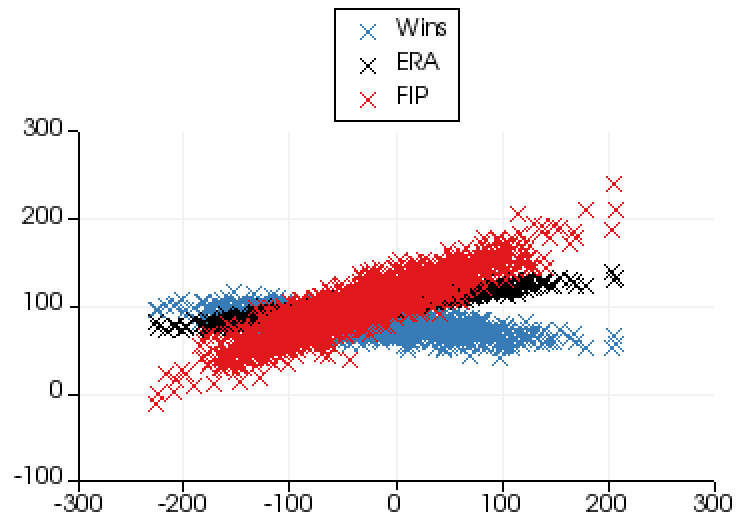
\includegraphics[width=0.9\linewidth]{similarpitch4} 
    \caption{Wins, ERA, FIP scaled} 
    \label{fig5:b} 
    \vspace{4ex}
  \end{subfigure} 
  \begin{subfigure}[b]{0.5\linewidth}
    \centering
    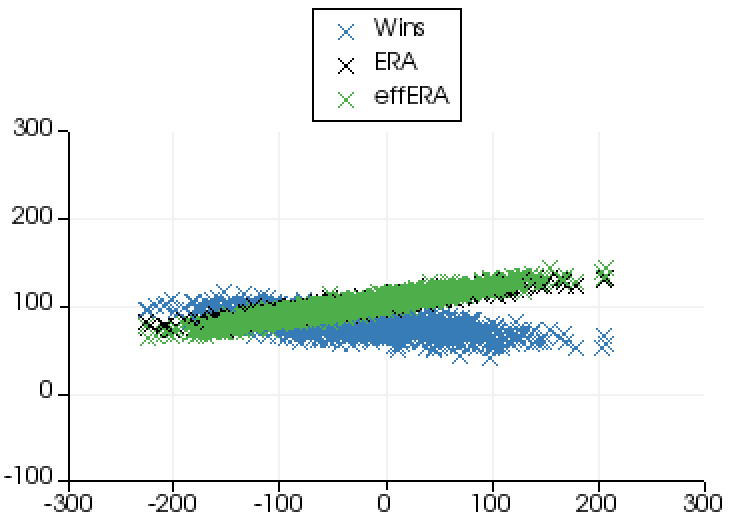
\includegraphics[width=0.9\linewidth]{similarpitch5} 
    \caption{Wins, ERA, effERA scaled} 
    \label{fig5:c} 
  \end{subfigure}%%
  \begin{subfigure}[b]{0.5\linewidth}
    \centering
    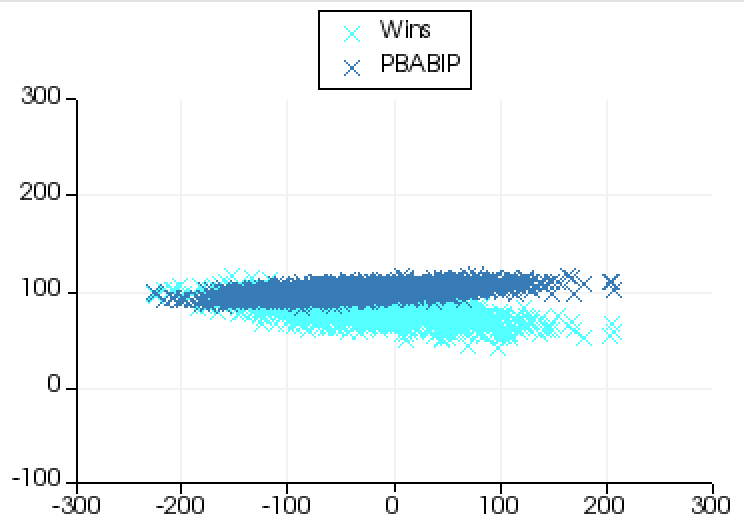
\includegraphics[width=0.9\linewidth]{similarpitch6} 
    \caption{Wins, PBABIP scaled} 
    \label{fig5:d} 
  \end{subfigure} 
  \caption{Similarity scores visualized on Paraview scaled to team pitching similarity scores}
  \label{fig5} 
\end{figure}


\noindent We see that the standard metrics with respect to the pitching similarity scores*, do not have a strong association, meaning they are not as good of an indicator to team performance. The sabremetrics however, have mixed results, with FIP being a great metric in associating team performance to pitching similarity scores. This is a much larger spread than the standard metrics, which suggests that we removed much of the noise. In addition, the effERA is nearly the same as the ERA in determining team performance near the middle, but differs from ERA at the extremas, potentially removing some noise in the ends due to bad luck or good luck or other environmental factors. \\

\noindent\textit{* to the 2015 Philadelphia Phillies}

\begin{figure}[H] 
  \begin{subfigure}[b]{0.5\linewidth}
    \centering
    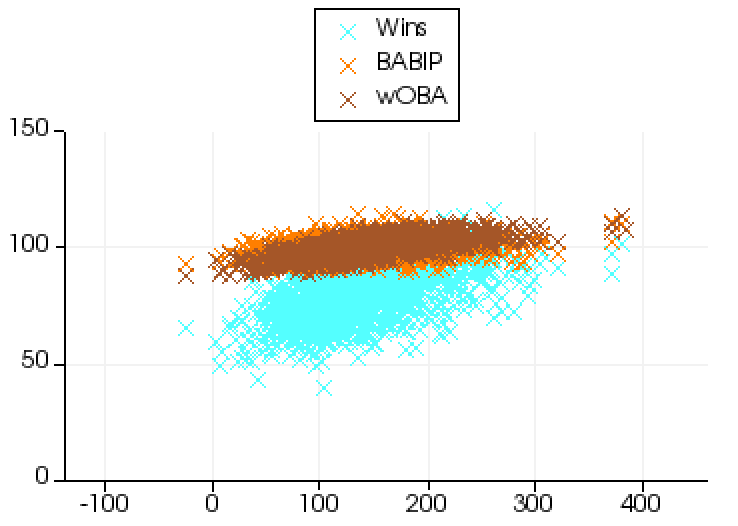
\includegraphics[width=0.9\linewidth]{similarhit1} 
    \caption{Wins, BABIP, wOBA} 
    \label{fig5:a} 
    \vspace{4ex}
  \end{subfigure}%% 
  \begin{subfigure}[b]{0.5\linewidth}
    \centering
    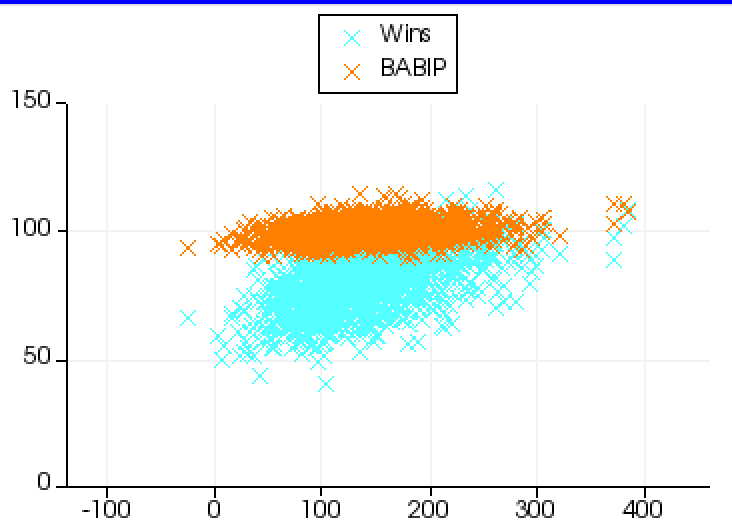
\includegraphics[width=0.9\linewidth]{similarhit2} 
    \caption{Wins, BABIP} 
    \label{fig5:b} 
    \vspace{4ex}
  \end{subfigure} 
  \begin{subfigure}[b]{\linewidth}
    \centering
    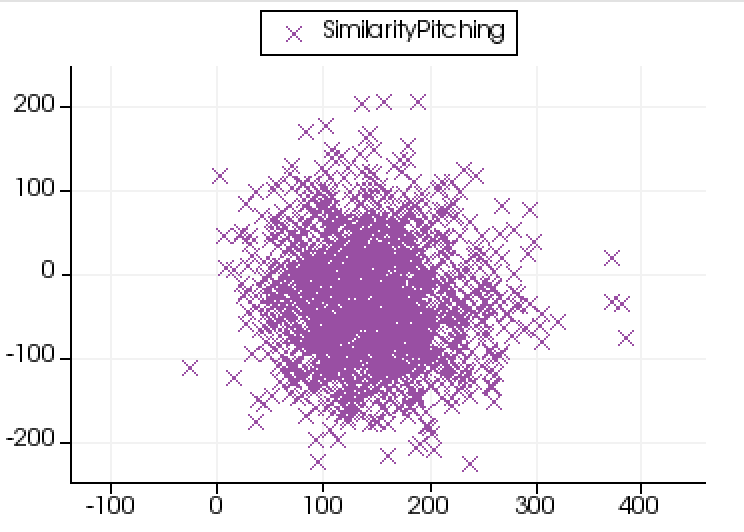
\includegraphics[width=0.6\linewidth]{similarhit4} 
    \caption{Similarity Pitching Scores} 
    \label{fig5:d} 
  \end{subfigure} 
  \caption{Similarity scores visualized on Paraview scaled to team batting similarity scores}
  \label{fig5} 
\end{figure}

We see now when we shift to similarity batting, the Wins is the only one with a deep association but at the cost of a wider spread. The BABIP and wOBA have a much shallower asssociation, but the spread is much tighter. When we look at the similarity pitching teams to the similarity batting, we see a good sign -- the association between the two is very weak. This confirms our scores calculated are independent.

Now, we centralize them to wins, such that the x-axis is team wins. Consider the results,

\begin{figure}[H] 
  \begin{subfigure}[b]{0.5\linewidth}
    \centering
    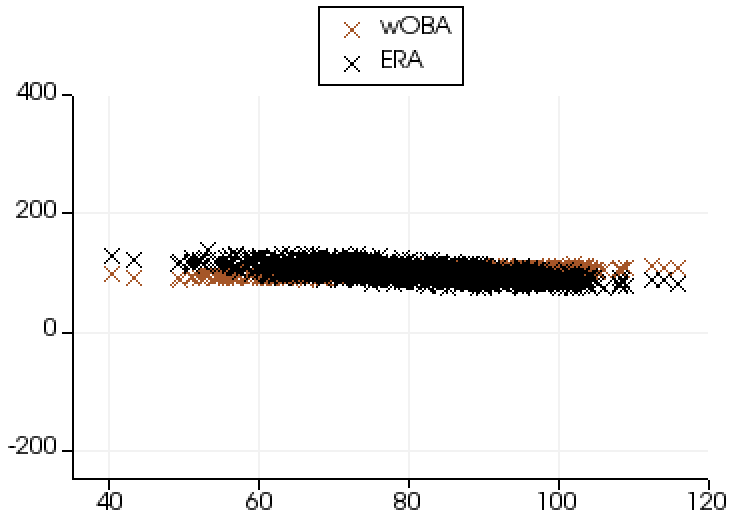
\includegraphics[width=0.9\linewidth]{wins2} 
    \caption{ERA, wOBA} 
    \label{fig5:a} 
    \vspace{4ex}
  \end{subfigure}%% 
  \begin{subfigure}[b]{0.5\linewidth}
    \centering
    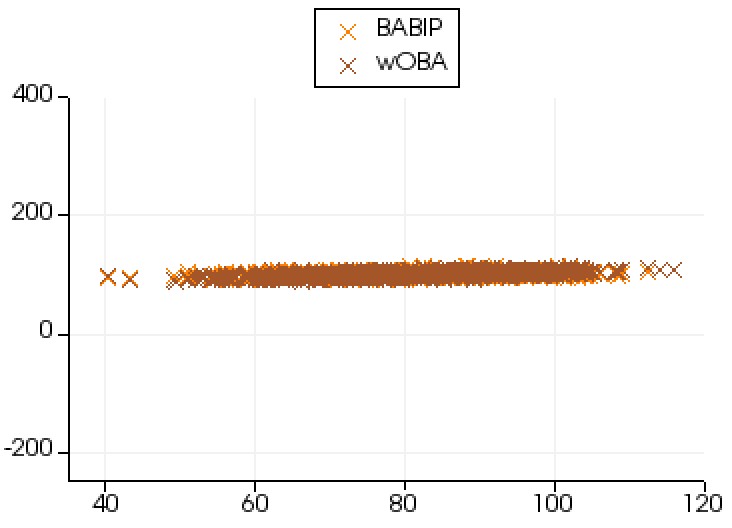
\includegraphics[width=0.9\linewidth]{wins3} 
    \caption{BABIP, wOBA} 
    \label{fig5:b} 
    \vspace{4ex}
  \end{subfigure} 
  \begin{subfigure}[b]{0.5\linewidth}
    \centering
    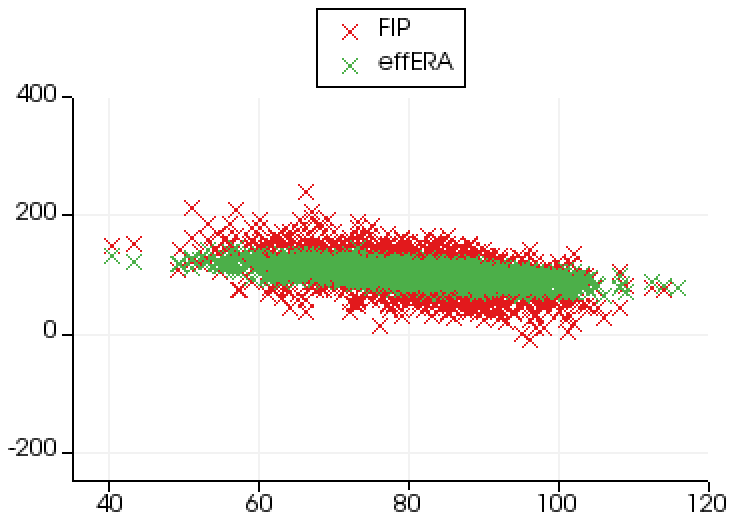
\includegraphics[width=0.9\linewidth]{wins4} 
    \caption{FIP, effERA} 
    \label{fig5:c} 
  \end{subfigure}%%
  \begin{subfigure}[b]{0.5\linewidth}
    \centering
    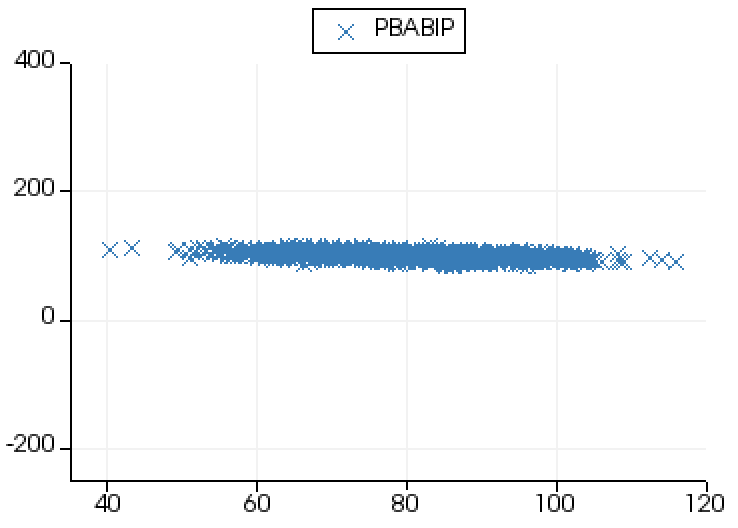
\includegraphics[width=0.9\linewidth]{wins5} 
    \caption{PBABIP} 
    \label{fig5:d} 
  \end{subfigure} 
  \caption{Similarity scores visualized on Paraview scaled to team wins in a 162 game season}
  \label{fig5} 
\end{figure}

\begin{figure}[H]
    \centering
    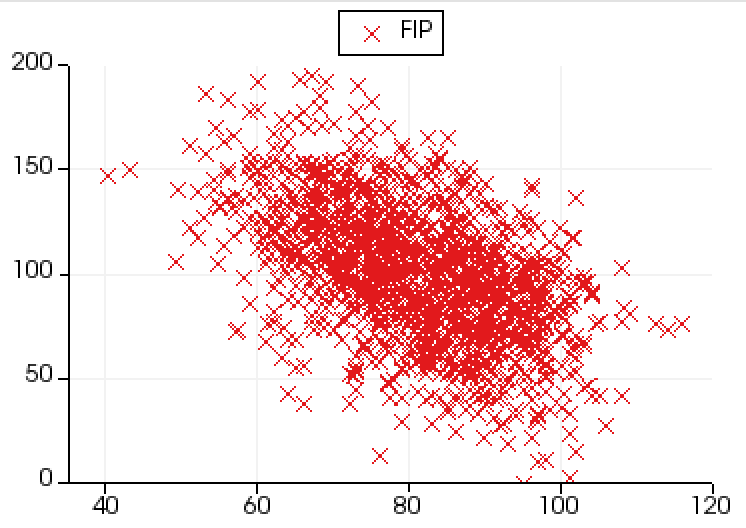
\includegraphics[width=0.5\linewidth]{wins8} 
    \caption{FIP vs. 162 expected team wins} 
\end{figure}

\noindent The FIP has the steepest association, but along with it's strength also has the largest spread.

\begin{figure}[H] 
  \begin{subfigure}[b]{0.5\linewidth}
    \centering
    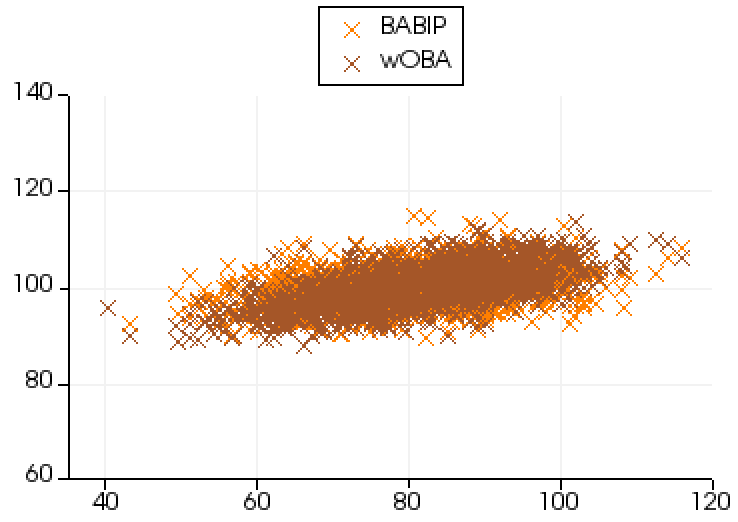
\includegraphics[width=0.9\linewidth]{wins6} 
    \captionsetup{justification=centering}
    \label{fig2:a} 
    \vspace{4ex}
  \end{subfigure}%% 
  \begin{subfigure}[b]{0.5\linewidth}
    \centering
    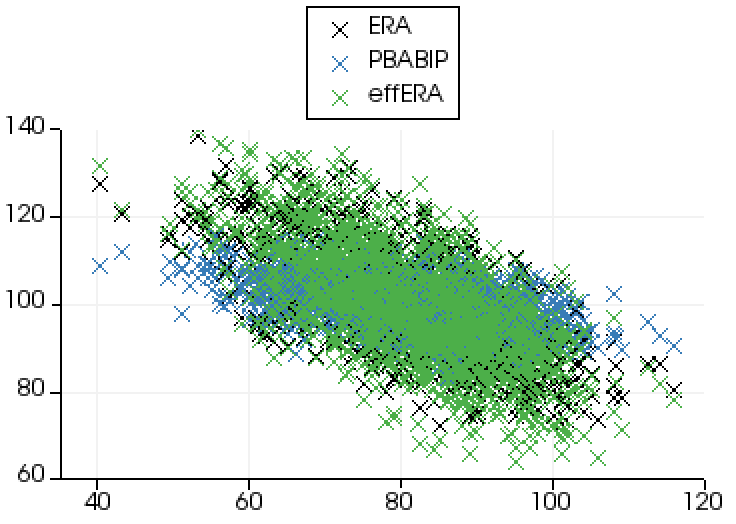
\includegraphics[width=0.9\linewidth]{wins7} 
    \captionsetup{justification=centering}
    \label{fig2:b} 
    \vspace{4ex}
  \end{subfigure}
  \centering
  \caption{More similarity scores visualized on Paraview scaled to team wins in a 162 game season}
\end{figure}

We attempted to do a 4D vector representation in Paraview, 
\begin{figure}[H]
    \centering
    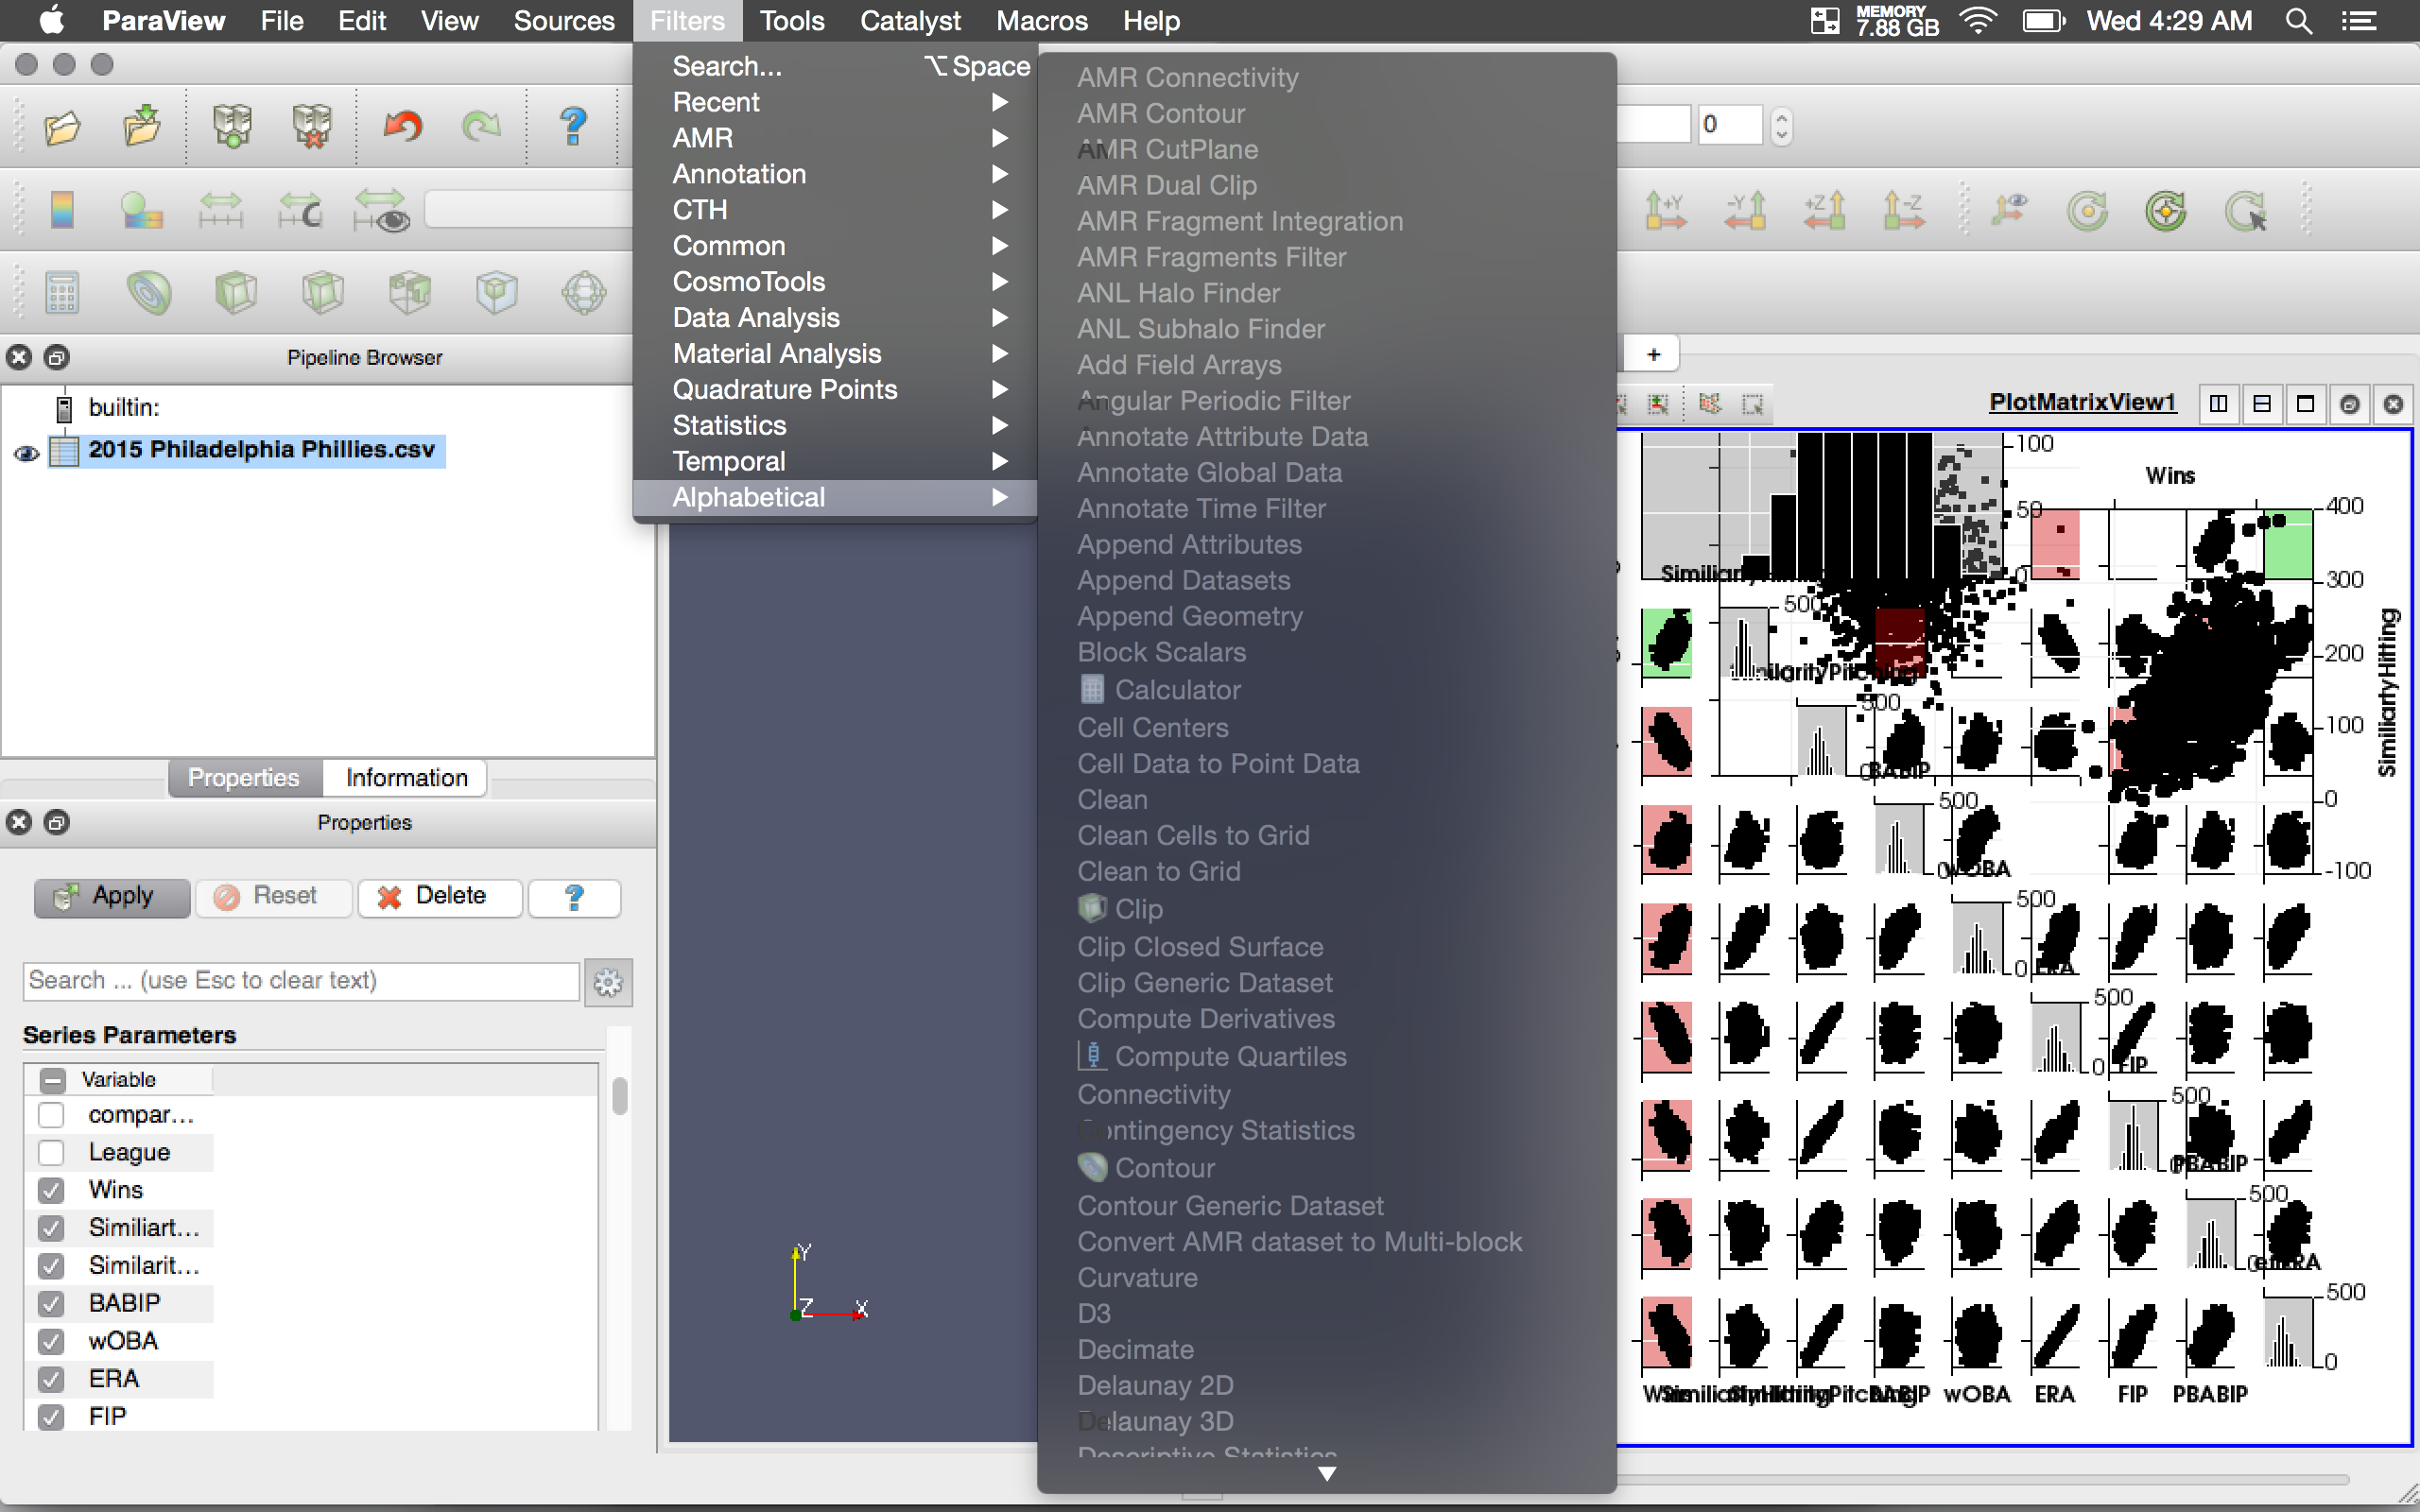
\includegraphics[width=0.5\linewidth]{no4d} 
    \caption{FIP vs. 162 expected team wins} 
\end{figure}

but could not after many attempts. Thus, we had to physically implement and draw from scratch in Python.

\subsection{3D Plots}
We then decided to visualize the calculated sabremetrics in three-dimensions to see if there were any clustering or similarities. First, we looked for pitching + batting team clusters.

\begin{figure}[H] 
\centering

  \begin{subfigure}[b]{0.33\linewidth}
    \centering
    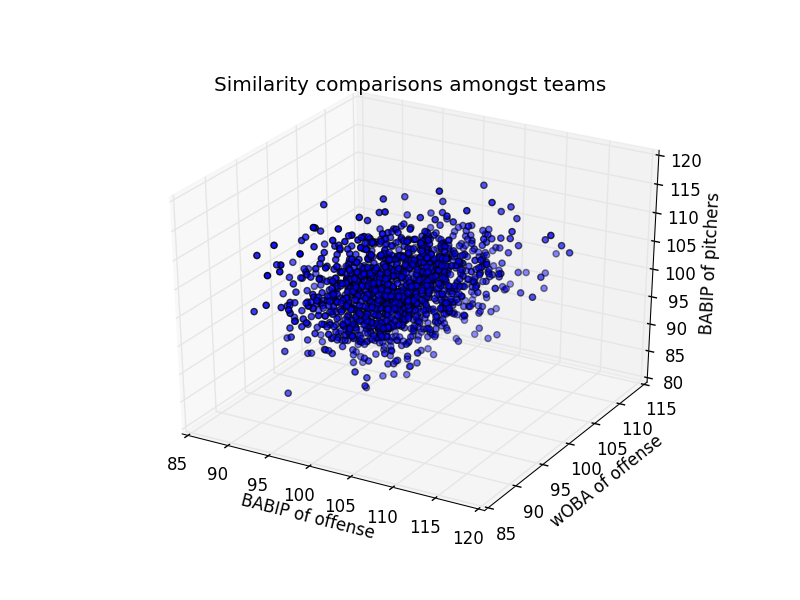
\includegraphics[width=0.9\linewidth]{Sim1} 
    \caption{BABIP, wOBA, PBABIP} 
    \label{fig5:a} 
    \vspace{4ex}
  \end{subfigure}%% 
  \begin{subfigure}[b]{0.33\linewidth}
    \centering
    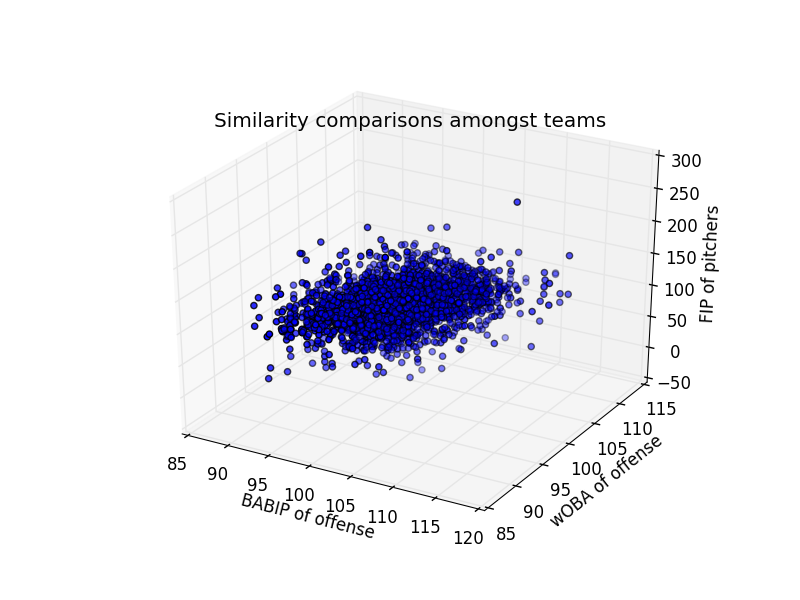
\includegraphics[width=0.9\linewidth]{Sim2} 
    \caption{BABIP, wOBA, FIP} 
    \label{fig5:b} 
    \vspace{4ex}
  \end{subfigure} 
  \begin{subfigure}[b]{0.33\linewidth}
    \centering
    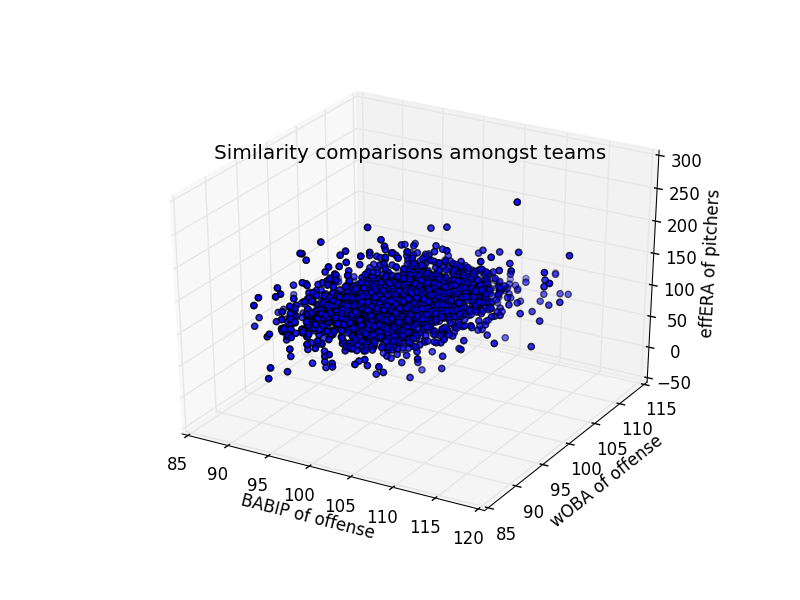
\includegraphics[width=0.9\linewidth]{Sim3} 
    \caption{BABIP, wOBA, effERA} 
    \label{fig5:c} 
    \vspace{4ex}
  \end{subfigure}
  
  \begin{subfigure}[b]{0.33\linewidth}
    \centering
    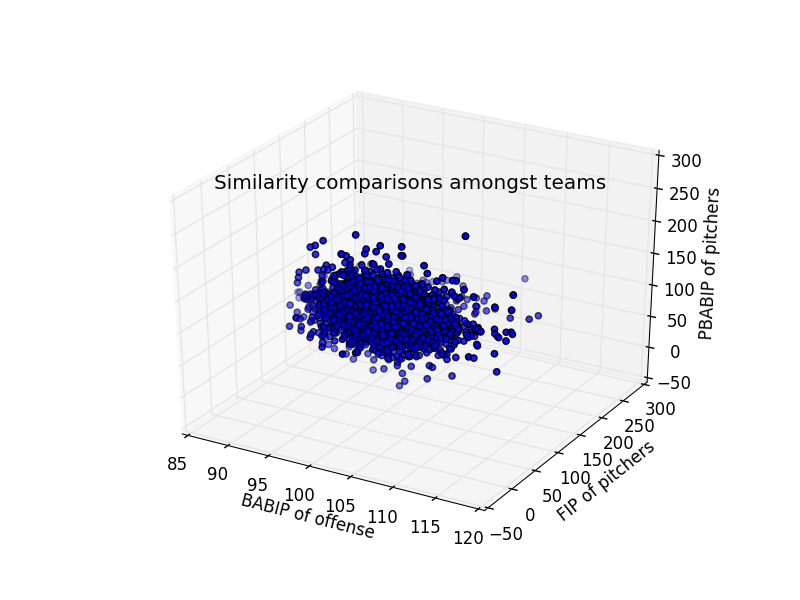
\includegraphics[width=0.9\linewidth]{Sim4} 
    \caption{BABIP, FIP, PBABIP} 
    \label{fig5:d} 
  \end{subfigure}%%
  \begin{subfigure}[b]{0.33\linewidth}
    \centering
    \includegraphics[width=0.9\linewidth]{Sim5} 
    \caption{wOBA, ERA, PBABIP} 
    \label{fig5:e} 
   \end{subfigure}
  \begin{subfigure}[b]{0.33\linewidth}
    \centering
    \includegraphics[width=0.9\linewidth]{Sim6} 
    \caption{FIP, ERA, PBABIP} 
    \label{fig5:f} 
  \end{subfigure} 
  \caption{Three Dimensional Visualization of Sabremetric statistics}
  \label{fig5}
\end{figure}

Looking at these plots, we can see that the data seems to be densely distributed, making any particular group hard to pull out. You will see that figure a has the highest chance of any particular clustering, while the rest seem to follow a normal distribution found in nature. Looking at purely the pitching statistics, we see that they are rather invariant of each other, all along the 100, 100, 100 axes. However, if you did make clustering groups, you'll find 6 neat K groups, but that does not give too much insight. We look into 2D visualizations next.

\begin{figure}[H] 
  \begin{subfigure}[b]{0.5\linewidth}
    \centering
    \includegraphics[width=0.9\linewidth]{Sim7} 
    \caption{wOBA, BABIP} 
    \label{fig5:a} 
    \vspace{4ex}
  \end{subfigure}%% 
  \begin{subfigure}[b]{0.5\linewidth}
    \centering
    \includegraphics[width=0.9\linewidth]{Sim8} 
    \caption{PBABIP, BABIP} 
    \label{fig5:b} 
    \vspace{4ex}
  \end{subfigure} 
  
  \begin{subfigure}[b]{0.5\linewidth}
    \centering
    \includegraphics[width=0.9\linewidth]{Sim9} 
    \caption{FIP, BABIP} 
    \label{fig5:c} 
  \end{subfigure}%%
  \begin{subfigure}[b]{0.5\linewidth}
    \centering
    \includegraphics[width=0.9\linewidth]{Sim10} 
    \caption{ERA, BABIP} 
    \label{fig5:d} 
  \end{subfigure} 
  \caption{Two dimensional visualization of sabremetrics}
  \label{fig5} 
 \end{figure}
  
  We find that in the offensive sabremetric comparisons, there seems to be some form of clustering due to the relatively large distribution along high wOBA and high BABIP, as well as low wOBA and low BABIP. This also applies to all the pitching stats and BABIP, with the one exception being PBABIP vs. BABIP. In this scenario, it seems that the clustering less significant, as it is more radially spread out. 
  
  
 Looking at wOBA now

\begin{figure}[H] 
  \begin{subfigure}[b]{0.5\linewidth}
    \centering
    \includegraphics[width=0.9\linewidth]{Sim11} 
    \caption{PBABIP, wOBA} 
    \label{fig5:a} 
    \vspace{4ex}
  \end{subfigure}%% 
  \begin{subfigure}[b]{0.5\linewidth}
    \centering
    \includegraphics[width=0.9\linewidth]{Sim12} 
    \caption{effERA, BABIP} 
    \label{fig5:b} 
    \vspace{4ex}
  \end{subfigure} 
  \begin{subfigure}[b]{0.5\linewidth}
    \centering
    \includegraphics[width=0.9\linewidth]{Sim13} 
    \caption{effERA, wOBA} 
    \label{fig5:c} 
  \end{subfigure}%%
  \begin{subfigure}[b]{0.5\linewidth}
    \centering
    \includegraphics[width=0.9\linewidth]{Sim14} 
    \caption{FIP, wOBA} 
    \label{fig5:d} 
  \end{subfigure} 
  \caption{Two dimensional visualization of sabremetrics (Cont.)}
  \label{fig5} 
\end{figure}

we can see that it has similar relations to that of pitching sabremetrics with BABIP, which confirms that these stats are respective of their binary categories (pitching or hitting). It is interesting to note that FIP has a larger spread than the other pitching categories, and that the spread increases as we go from ERA (traditional) to the most extreme of sabremetrics (FIP). This likely shows that ERA suppresses information within the dataset. Furthermore, we note that many of the datapoints do not change -- I think this is an error, and I will need to rerun again.

\section{4D Plots}
To further look into data, now comparing to wins, we consider a 4D dataset. We originally wanted to look at a 3D dataset, analyzing similarity wins to similarity pitching to wins in a 162 game season, but instead, we are looking at an additional variable, BABIP. We chose BABIP because of it's moderate association relative to the rest of the dataset. 

\begin{figure}[H]
	\centering
    \includegraphics[width=0.9\linewidth]{4d5}
    \caption{4D visual representation of key baseball metrics}
\end{figure}

This plot is a preliminary plot showing the relative degree of information of from pitching similarity, batting similarity, BABIP, and color scaled by wins. You can see that the colors are grouped near each other, in sections. This is the first instance of potential success in k-clustering.  So, we further examine using a 3D mapping with color for geography.

\begin{figure}[H] 
  \begin{subfigure}[b]{0.5\linewidth}
    \centering
    \includegraphics[width=0.9\linewidth]{4d1} 
    \label{fig5:a} 
    \vspace{4ex}
  \end{subfigure}%% 
  \begin{subfigure}[b]{0.5\linewidth}
    \centering
    \includegraphics[width=0.9\linewidth]{4d2} 
    \label{fig5:b} 
    \vspace{4ex}
  \end{subfigure} 
  \begin{subfigure}[b]{0.5\linewidth}
    \centering
    \includegraphics[width=0.9\linewidth]{4d3} 
    \label{fig5:c} 
  \end{subfigure}%%
  \begin{subfigure}[b]{0.5\linewidth}
    \centering
    \includegraphics[width=0.9\linewidth]{4d4} 
    \label{fig5:d} 
  \end{subfigure} 
  \caption{4 dimensional visualization of sabremetrics$^+$}
  \label{fig5} 
\end{figure}

\noindent with axes being the same as above,
\begin{itemize}
	\item X = pitching similarity scores
    \item Y = hitting similarity scores
    \item Z = normalized BABIP
    \item C = projected 162 season wins
\end{itemize}

and we something quite interesting here. We can see some significant clustering in win values along the X-Y plane and this is not significantly dependent on BABIP (our Z-axis). The coloring, representing wins, is group relative to one another, the most wins in particularly one corner, while the least wins wrapping around another corner. However, there is some significant clustering along the z-axis, too. This is a comparative sign that BABIP can be used for a clustering algorithm. It's interesting to observe the purple group or least wins group was isolated around the corners, and underneath the most wins groups. The teams with average wins varied around the center and surface, while the most and least wins encompassed the corners. \\

\noindent\textit{Note the scale is off on the color in terms of value. I attempted to fix it for a couple hours and had no avail. The coloring and grouping is correct, but the display and values is not. The red or top part of the color scheme represents the most wins, while the bottom part of the color scheme or purple represented the least projected wins in a 162 game season.}\\

\noindent\textit{$^+$See full graphic picture below. The visualization is clear and the interpretation is stunning.}


\section{K-means Clustering}
Because I saw some form of partition within our data, I decided to see if there were an classifications of the dataset by doing a K-means Clustering, specifically focusing on the offensive statistics. The k-means algorithm takes a dataset $X$ of $N$ points as input, and makes $K$ clusters to create. The output is a set of $K$ cluster centroids and each cluster containing datapoints from our dataset $X$.

Mathematically, this means 

\begin{equation}
	Min \sum_{k=1}^{K}\sum_{x_n\epsilon C_k}^{}\left \| x_n-\mu _k \right \|^2 \text{with respect to} \ \ C_k,\mu _k
\end{equation}

Specifically, I used Lloyd's algorithm \cite{kmeans}\cite{kmeans2} which can be expressed as so:

\begin{figure}[H]
	\begin{subfigure}[b]{\linewidth}
		\centering
		\includegraphics[width=0.6\textwidth]{lloyd1}
        \end{subfigure}
    \begin{subfigure}[b]{\linewidth}
    	\centering
		\includegraphics[width=0.20\textwidth]{lloyd2}
    \end{subfigure}
\end{figure}

and by partitioning from $K=3$ to $K=6$, we get the following
\begin{figure}[H] 
  \begin{subfigure}[b]{0.5\linewidth}
    \centering
    \includegraphics[width=0.9\linewidth]{KCluster1} 
    \caption{K = 5} 
    \label{fig5:a} 
    \vspace{4ex}
  \end{subfigure}%% 
  \begin{subfigure}[b]{0.5\linewidth}
    \centering
    \includegraphics[width=0.9\linewidth]{KCluster2} 
    \caption{K = 4} 
    \label{fig5:b} 
    \vspace{4ex}
  \end{subfigure} 
  \begin{subfigure}[b]{0.5\linewidth}
    \centering
    \includegraphics[width=0.9\linewidth]{KCluster3} 
    \caption{K = 3} 
    \label{fig5:c} 
  \end{subfigure}%%
  \begin{subfigure}[b]{0.5\linewidth}
    \centering
    \includegraphics[width=0.9\linewidth]{KCluster4} 
    \caption{K = 6} 
    \label{fig5:d} 
  \end{subfigure} 
  \caption{K Clustering for wOBA vs. BABIP}
  \label{fig5} 
\end{figure}

We can see that at $K=3$ and $K=4$, the $K$ values were not significant enough to consider grouping these datasets. However, at $K>5$, this is where we start to see teams group together. We are careful not to go over $K=6$ because having large $K$ can make sets seem unique to group, but rather muddies the relationships as groupings become more individualized.

When we compared a select number of these datapoints to their similarity scores, we found that they seemed to group together (within a respectable range) in the offensive similarity. Applying the same study to some pitching sabremetrics showed similar results.

This suggests that our similarity algorithm was decent at finding similar teams, although the range was large enough to warrant a future calibrating of coefficients in our similarity calculator.\\

\noindent And comparing the $k=5$ clustering results using Paraview

\begin{figure}[H]
	\centering
    \includegraphics[width=0.9\linewidth]{cluster1}
    \caption{Cluster 1, yellow}
\end{figure}

\noindent We can see that there's a definite cluster in both our histogram databin and our scatter plot. The histogram in the top left corner represents the x-axis, while the histogram on the bottom right represent the y-axis. The scatterplot on the top right represents a density scatterplot, similar to that of the scatterplot describing our K-means clustering, while the scatterplot on the bottom left represents a weighted density plot with the increments being distributed to account for density of regions. The bins in the histogram suggest a rather tight distribution. It is not quite exactly normal due to it's relative location to the other clusters (it's skewed), but is close to being normally distributed because of the nature of the dataset (team performance).

\begin{figure}[H] 
  \begin{subfigure}[b]{0.5\linewidth}
    \centering
    \includegraphics[width=0.9\linewidth]{cluster2} 
    \caption{cluster 2, red} 
    \label{fig5:a} 
    \vspace{4ex}
  \end{subfigure}%% 
  \begin{subfigure}[b]{0.5\linewidth}
    \centering
    \includegraphics[width=0.9\linewidth]{cluster3} 
    \caption{cluster 3, blue} 
    \label{fig5:b} 
    \vspace{4ex}
  \end{subfigure} 
  \begin{subfigure}[b]{0.5\linewidth}
    \centering
    \includegraphics[width=0.9\linewidth]{cluster4} 
    \caption{cluster 4, green} 
    \label{fig5:c} 
  \end{subfigure}%%
  \begin{subfigure}[b]{0.5\linewidth}
    \centering
    \includegraphics[width=0.9\linewidth]{cluster5} 
    \caption{cluster 5, cyan} 
    \label{fig5:d} 
  \end{subfigure} 
  \caption{Analyzing each individual k-cluster}
  \label{fig5} 
\end{figure}

We can see that like the first cluster, each one of these clusters, when isolated, seemed to be appropriately distributed or clumped, based on the nature of the histograms and the density of the scatterplots. The information or data becomes much clearer when isolated from the other $k_i$ clusters. Most of the $k_i$ clusters look appropriate.

\section{Future work}
From this finding, we can now move on to further analysis. Our current algorithm for similarity looks good, but the coefficients may need to be rerun on known sets to tweak to obtain a certain accuracy. We may also want to include ballpark effects -- every ballpark has a factor that affects batting and pitching performances. Once this is done, we can then modify these files to work on individual player data. This can first be written in python, but eventually may need to be moved into R for more visualization. We predict that player similarities should be more obvious as even basic offensive categories creates groups of people (ie. sluggers, fast runners, 5 tool, etc), and the k-mean clustering algorithm would produce more obtuse results. Different clusters of players should have have similar stats (remember, we use normalized remember, not RAW). \textit{The ballpark effect will have a more prominent effect and use for individual players}.

Once the similarity can be run on players, we can then then run test sets found from queries made on the database, and apply machine learning until we get the correct coefficients. Then, we apply this to a non-test set to yield results for any players throughout any duration of time. These similar player stats will be combined for the seasons after the similar years, and we will then use this statistic to project production and performance down the road for the target player. \textit{Note we cannot apply this extrapolation to teams, because teams vary to a degree that extrapolating provides no additional important information}.

Note, similarity scores for teams could also be used down the road. For the projections of wins or successes in the new season, we can consider taking the new roster and statistics from the previous season and run the program the same way.

\pagebreak

\centering{Github R snippets}
\begin{lstlisting}[language=R, caption=Github R snippets]
# track the number of pitches per game (for each pitcher-type combination)
n_pitches <- pitches %>%
  group_by(pitch_type, pitcher_name, date) %>%
  summarise(count = n()) %>% 
  mutate(group = paste(pitcher_name, pitch_type, sep = ": ")) %>%
  mutate(dated = as.Date(date, format = "%Y_%m_%d")) %>%
  data.frame %>% mutate(max_n = max(count))

# time series plot with clickSelects
series <- ggplot() + 
  geom_line(aes(x = dated, y = count, colour = pitch_type, 
                linetype = pitcher_name, group = group), data = n_pitches) + 
  stat_identity(aes(x = dated, y = max_n, clickSelects = date, alpha = 0.2), 
                geom = "bar", data = n_pitches) + scale_alpha(guide = 'none') +
  xlab("") + ylab("Number of pitches") + theme_animint(width = 800, height = 200)

plist2 <- list(strike = strike,
               strikeDate = strike_date,
               series = series,
               selector.types = list(date = "multiple"))

structure(plist2, class = "animint")
\end{lstlisting}
\bigskip
\centering{Rstudio snippets}
\begin{lstlisting}[language=R, caption=Rstudio R snippets]
library(splines)
library(arm)
library(pitchRx)
library(dplyr)
library(reshape2)

#Download data.
start = "2014-07-01"
end = "2014-10-01"

db <- src_sqlite("pitchfx.sqlite3", create=TRUE)
#Uncomment to download data only needs to happen once.
pitches <- scrape(start=start, end=end, connect=db$con)

#Select only the setup and strikeout pitches.
abs <- tbl(db, sql("SELECT * FROM atbat WHERE  date > '2014-03-01'"))
pitches_ <- tbl(db, sql("SELECT * FROM pitch"))

#Join on atbat info.
abs <- inner_join(abs, pitches_, by=c("gameday_link", "num"))

#Need to join pitches, with setup pitches.
z <- collect(abs) #Need to use rank, not implemented in sqlite.

y <- rbind_list(mutate(z, lbl='last'),
                mutate(z, lbl='setup')) %>%
     arrange(lbl, gameday_link, num, id) %>%
     group_by(lbl, gameday_link, num) %>%
     mutate(rk = rank(id),
            rrank=rank(id) - max(rk),
            rrank = ifelse(lbl=='setup', rrank+1, rrank)
            ) %>%
    filter(lbl %in% c('setup', 'last') & rk > 1 & rrank < 1) %>%
    select(gameday_link, num, rrank, pitch_type, lbl, start_speed,
           count, event, des, px, pz, stand, p_throws, pitcher, count) %>%
    melt(id.vars=c('gameday_link', 'num', 'rrank', 'lbl')) %>%
    dcast(gameday_link + num + rrank  ~ variable + lbl) %>%
    filter(!is.na(event_setup))

#Independent of other variables, what pitches "set up" others best for swings and misses?
strikeouts <- y%>%
    mutate(swinging_k = des_last %in% c('Swinging Strike', 'Swinging Strike (Blocked)'),
           called_k = des_last=='Called Strike',
           speed_change = as.numeric(start_speed_last) - as.numeric(start_speed_setup),
           x_change = ifelse(stand_last=='L', -1, 1) * (as.numeric(px_last) - as.numeric(px_setup)),
           y_change = as.numeric(pz_last) - as.numeric(pz_setup))
\end{lstlisting}

\bigskip
\centering{Similarity of Teams}
\begin{lstlisting}[language=Python, caption=Similarity Algorithm]
import csv
import pandas as pd
from math import isnan
import os
from sys import exit
import argparse
import numpy as np
 
dataFile = "/Users/kaichang/Documents/classes/ay119/final_project/lahman-csv/Teams.csv"
years, numSeasons, teamNames, league, gamesPlayed, teamWins, R, AB, H, doubles, triples, HR, BB, SO, SB, CS, HBP, SF, ERA, IPouts, BBA, SOA, HRA, HA, CG, SHO, SV, FP, E, DP, BPF, PPF, ER, avg, sums = readDatabase(dataFile)
header = ["comparedTeam", "League", "Wins", "SimiliartyHitting", "SimilarityPitching","BABIP","wOBA","ERA","FIP","PBABIP","effERA"]
dir = "results/"
if not os.path.exists(dir): # create results directory if it doesn't exist already 
    os.makedirs(dir)
createOutputFiles(years, teamNames, numSeasons)

# compare teams, calculate scores, and write the scores to a file    
# starts at 2012
for j in range (2686, numSeasons):
        year1, team1, lg1, projwins1, BABIPPlus1, wOBAPlus1, OBPPlus1, SLGPlus1, KPPlus1, BBPPlus1, RPPlus1, HRPPlus1, SBCSRatePlus1, ERAPlus1, WHIPPlus1, HP9Plus1, BBP9Plus1, KP9Plus1, FIPPlus1, PBABIPPlus1, effERAPlus1, CGratePlus1 = getTeamInfo(years, teamNames, league, gamesPlayed, teamWins, R, AB, H, doubles, triples, HR, BB, SO, SB, CS, HBP, SF, ERA, IPouts, BBA, SOA, HRA, HA, CG, SHO, SV, FP, E, DP, BPF, PPF, ER, avg, j)
        id1 = str(year1) + ' ' + team1
        if args.verbose:
            print "Comparison team: %s" %id1
        fileToOpen = os.path.join(dir, id1) + '.csv'
        try:
            # Open Team J's results file for writing
            f = open(fileToOpen, 'a')
            results = csv.writer(f)
            row = [id1, lg1, projwins1, 100, 100, BABIPPlus1, wOBAPlus1, ERAPlus1, FIPPlus1, PBABIPPlus1, effERAPlus1]
            results.writerow(row)
            #runs and checks similarities dating back to 1960
            for k in range (1344, numSeasons):
                year2, team2, lg2, projwins2, BABIPPlus2, wOBAPlus2, OBPPlus2, SLGPlus2, KPPlus2, BBPPlus2, RPPlus2, HRPPlus2, SBCSRatePlus2, ERAPlus2, WHIPPlus2, HP9Plus2, BBP9Plus2, KP9Plus2, FIPPlus2, PBABIPPlus2, effERAPlus2, CGratePlus2 = getTeamInfo(years, teamNames, league, gamesPlayed, teamWins, R, AB, H, doubles, triples, HR, BB, SO, SB, CS, HBP, SF, ERA, IPouts, BBA, SOA, HRA, HA, CG, SHO, SV, FP, E, DP, BPF, PPF, ER, avg, k)
                id2 = str(year2) + ' ' + team2                
                if (id1 != id2): # prevent comparing a team to itself
                    row = [] # start a blank row for a new comparison
                    row.append(id2) #add the comparison team as the first column
                    row.append(lg2)
                    row.append(projwins2)
                    simScoreHit = compareTeamsHitting(wOBAPlus1, wOBAPlus2, BABIPPlus1, BABIPPlus2, OBPPlus1, OBPPlus2, SLGPlus1, SLGPlus2, RPPlus1, RPPlus2, KPPlus1, KPPlus2, BBPPlus1, BBPPlus2, HRPPlus1, HRPPlus2, SBCSRatePlus1, SBCSRatePlus2)
                    row.append(simScoreHit)
                    simScorePitch = compareTeamsPitching(ERAPlus1, ERAPlus2, FIPPlus1, FIPPlus2, WHIPPlus1, WHIPPlus2, KP9Plus1, KP9Plus2, BBP9Plus1, BBP9Plus2, HP9Plus1, HP9Plus2, PBABIPPlus1, PBABIPPlus2, effERAPlus1, effERAPlus2)
                    row.extend((simScorePitch,BABIPPlus2,wOBAPlus2,ERAPlus2,FIPPlus2,PBABIPPlus2,effERAPlus2))
                    results.writerow(row)
        except Exception as e:
            print "Error opening %s: %s" % (fileToOpen, e) 
        f.close() #we are done with team J's CSV file.  
\end{lstlisting}

\bigskip

\centering{3D Visualization}
\begin{lstlisting}[language=Python, caption=3D Visualization]
import pandas as pd  # (*) pandas for dataframe manipulation
import csv
import matplotlib.pyplot as plt # module for plotting 
import sklearn
import scipy
import numpy as np

from mpl_toolkits.mplot3d import Axes3D




dataFile = "/Users/kaichang/Documents/classes/ay119/final_project/baseball-team-similarity-master/results/2015 Philadelphia Phillies.csv"
df = pd.read_csv(dataFile, sep=',')

#df = df.drop(df.index[0])  # drop first row (US totals) 
#df = df[df['murder'] < 11] # drop out-of-range rows

fig = plt.figure()         # (!) set new mpl figure object
ax = fig.add_subplot(111, projection='3d')  # add axis

ax.set_xlabel('BABIP of offense')
ax.set_ylabel('wOBA of offense')
ax.set_zlabel('BABIP of pitchers')
plt.title('Similarity comparisons amongst teams')

scatter = ax.scatter(
    df['BABIP'], 
    df['wOBA'], 
    df['PBABIP'],
    # linewidths=2, 
    # edgecolor='w',
    # alpha=0.6
)

#plt.show()
plt.savefig('Sim1.png')
\end{lstlisting}

\bigskip
\centering{4D Visualization}

\begin{lstlisting}[language=Python, caption=4D Visualization (3d color mapping)]
import matplotlib
import matplotlib.pyplot as plt
import pandas as pd  # (*) pandas for dataframe manipulation
import csv
import matplotlib.pyplot as plt # module for plotting 
import sklearn
import scipy
import numpy as np
from matplotlib import cm
import matplotlib.colors as colors
from mpl_toolkits.mplot3d import Axes3D
import pylab
from scipy.interpolate import griddata


dataFile = "/Users/kaichang/Documents/classes/ay119/final_project/baseball-team-similarity-master/results/2015 Philadelphia Phillies.csv"
df = pd.read_csv(dataFile, sep=',')

#df = df.drop(df.index[0])  # drop first row (US totals) 
#df = df[df['murder'] < 11] # drop out-of-range rows

fig = matplotlib.pyplot.gcf()
ax1 = fig.add_subplot(111, projection='3d')  # add axis
#ax1.set_zlabel('BABIP of offense')
#ax1.set_ylabel('wOBA of offense')
#ax1.set_xlabel('BABIP of pitchers')
ax1.set_xlabel('Pitching Similarity Scores')
ax1.set_ylabel('Hitting Similarity Scores')
ax1.set_zlabel('BABIP')
#plt.title('Similarity comparisons amongst teams')

Z = df['BABIP']
#Y = df['wOBA'] 
#X = df['PBABIP']
X = df['SimilarityPitching']
Y = df['SimiliartyHitting']
#Z = df['Wins']
C = df['Wins']

xi = np.linspace(X.min(),X.max(),100)
yi = np.linspace(Y.min(),Y.max(),100)
#zi = np.linspace(Z.min(),Z.max(),100)
#ci = np.linspace(C.min(),C.max(),100)
ci = griddata((X, Y), C, (xi[None,:], yi[:,None]), method='cubic')
zi = griddata((X, Y), Z, (xi[None,:], yi[:,None]), method='cubic')


norm = colors.Normalize(vmin=C.min(),vmax=C.max())
xig, yig = np.meshgrid(xi, yi)
surf = ax1.plot_surface(xig, yig, zi,facecolors=cm.rainbow(norm(ci)), alpha=0.7)

m = cm.ScalarMappable(cmap=cm.rainbow)
m.set_array(np.unique(ci))
col = plt.colorbar(m)
plt.show()

#ax1.scatter(X,Y,Z,c=C)
#plt.show()
\end{lstlisting}

\bigskip
\centering{K-means Clustering}
\begin{lstlisting}[language=Python, caption=K-means Clustering]
import pandas as pd  # (*) pandas for dataframe manipulation
import csv
import matplotlib.pyplot as plt # module for plotting 
import sklearn
import scipy
import numpy as np
import random

from mpl_toolkits.mplot3d import Axes3D

def cluster_points(X, mu):
    clusters  = {}
    for x in X:
        bestmukey = min([(i[0], np.linalg.norm(x-mu[i[0]])) \
                    for i in enumerate(mu)], key=lambda t:t[1])[0]
        try:
            clusters[bestmukey].append(x)
        except KeyError:
            clusters[bestmukey] = [x]
    return clusters

def reevaluate_centers(mu, clusters):
    newmu = []
    keys = sorted(clusters.keys())
    for k in keys:
        newmu.append(np.mean(clusters[k], axis = 0))
    return newmu
 
def has_converged(mu, oldmu):
    return (set([tuple(a) for a in mu]) == set([tuple(a) for a in oldmu]))

def find_centers(X, K):
    # Initialize to K random centers
    oldmu = random.sample(X, K)
    mu = random.sample(X, K)
    while not has_converged(mu, oldmu):
        oldmu = mu
        # Assign all points in X to clusters
        clusters = cluster_points(X, mu)
        # Reevaluate centers
        mu = reevaluate_centers(oldmu, clusters)
    return(mu, clusters)
\end{lstlisting}


\pagebreak

\section{Full Graphics Vectors}

\begin{figure}[H]
	\centering
    \includegraphics[width=0.9\linewidth]{4d1}
    \caption{4D Representation}
\end{figure}

\begin{figure}[H]
	\centering
    \includegraphics[width=0.9\linewidth]{4d2}
    \caption{4D Representation cont.}
\end{figure}

\begin{figure}[H]
	\centering
    \includegraphics[width=0.9\linewidth]{4d3}
    \caption{4D Representation cont.}
\end{figure}

\begin{figure}[H]
	\centering
    \includegraphics[width=0.9\linewidth]{4d4}
    \caption{4D Representation cont.}
\end{figure}

\begin{figure}[H]
	\centering
    \includegraphics[width=0.9\linewidth]{KCluster1}
    \caption{K=5 Clustering}
\end{figure}


\pagebreak
\normalsize
\bibliographystyle{unsrt}
\begin{thebibliography}{1}
	\bibitem{sloan} Gartheeban, Ganeshapillai, and John Guttag. "A Data-driven Method for In-game Decision Making in MLB." Proceedings of the 19th ACM SIGKDD International Conference on Knowledge Discovery and Data Mining - KDD '13 (2013): n. pag. Web. %http://www.sloansportsconference.com/wp-content/uploads/2014/02/2014_SSAC_Data-driven-Method-for-In-game-Decision-Making.pdf
    \bibitem{BYBS}"Saberizing a Mac \#6: Calculating FIP, FIP-, ERA-." Beyond the Box Score. N.p., 24 Jan. 2013. Web. May 2016. %\<http://www.beyondtheboxscore.com/2013/1/24/3909282/saberizing-a-mac-6-calculating-fip-fip-era\>. 
    \bibitem{FIP}"FIP | FanGraphs Sabermetrics Library." FIP | FanGraphs Sabermetrics Library. N.p., n.d. Web. May 2016.  %<http://www.fangraphs.com/library/pitching/fip/>. 
    \bibitem{kmeans}  "Clustering With K-Means in Python." The Data Science Lab. N.p., 12 Dec. 2013. Web. May 2016. %https://datasciencelab.wordpress.com/2013/12/12/clustering-with-k-means-in-python/
    \bibitem{kmeans2} "K-means Clustering¶." K-means Clustering — Scikit-learn 0.17.1 Documentation. N.p., n.d. Web. May 2016. %http://scikit-learn.org/stable/auto_examples/cluster/plot_cluster_iris.html
    \bibitem{fangraphs}"WOBA | FanGraphs Sabermetrics Library." WOBA | FanGraphs Sabermetrics Library. N.p., n.d. Web. Apr. 2016. %http://www.fangraphs.com/library/offense/woba/
    \bibitem{BaseballReference}"Park Adjustments | Baseball-Reference.com." Baseball-Reference.com. N.p., n.d. Web. 2016.  %<http://www.baseball-reference.com/about/parkadjust.shtml>. 
    \bibitem{Bales} Bales, John. "Most Important Stats: Batting." Most Important Stats: Batting. N.p., n.d. Web. May 2016. %https://rotogrinders.com/lessons/most-important-stats-batting-268627
    \bibitem{BABIP} "BABIP | FanGraphs Sabermetrics Library." BABIP | FanGraphs Sabermetrics Library. N.p., n.d. Web. May 2016.  %<http://www.fangraphs.com/library/pitching/babip/>.
    \bibitem{PCA}  "Principal Component Analysis Explained Visually." Explained Visually. N.p., n.d. Web. May 2016. %http://setosa.io/ev/principal-component-analysis/
    \bibitem{StackOverflow} "Matplotlib Correct Colors/colorbar for Plot with Multiple Surfaces Each of a Different Color." Python. N.p., n.d. Web. June 2016. %http://stackoverflow.com/questions/35569833/matplotlib-correct-colors-colorbar-for-plot-with-multiple-surfaces-each-of-a-dif

    
\end{thebibliography}
\end{document}